\documentclass{article}

\usepackage{iclr2027_conference,times}
\usepackage{amsmath,amssymb,amsthm}
\usepackage{array}
\usepackage{booktabs}
\usepackage{etoolbox}
\usepackage{graphicx}
\usepackage{hyperref}
\usepackage{url}
\usepackage{microtype}
\usepackage{float}
\hypersetup{hidelinks,hypertexnames=false}
\setlength{\textfloatsep}{3pt plus 1pt minus 1pt}
\setlength{\floatsep}{3pt plus 1pt minus 1pt}
\setlength{\intextsep}{3pt plus 1pt minus 1pt}
\setlength{\abovedisplayskip}{6pt plus 1pt minus 1pt}
\setlength{\belowdisplayskip}{6pt plus 1pt minus 1pt}
\AtBeginEnvironment{table}{\small}
\renewcommand{\arraystretch}{1.02}

\title{Latent State Spectral Transfer:\\Supplementary Material}
\author{Anonymous Authors}
\date{}

\DeclareMathOperator{\tr}{tr}
\newcommand{\comm}[2]{[#1,#2]}
\newcommand{\R}{\mathbb{R}}
\renewcommand{\theequation}{S\arabic{equation}}
\newtheorem{supptheorem}{Theorem}
\newtheorem{suppprop}[supptheorem]{Proposition}

\begin{document}
\maketitle

\section{Supplementary Results and Derivations}

This supplement gives the derivations, analytical sweeps, learned-representation measurements, intervention boundaries, and temporal evaluation protocols used in the main manuscript. Sections~\ref{sec:supp-derivation}--\ref{sec:supp-null} derive and test the same-spectrum commutator identity; Sections~\ref{sec:supp-ablation}--\ref{sec:supp-robustness} separate alignment from spectral shape and examine robustness; and Section~\ref{sec:supp-auxiliary} provides an additional spectrum-fixed subspace diagnostic. Sections~\ref{sec:supp-frozen-pusht}--\ref{sec:supp-intervention} analyze frozen LeWorldModel representations and the prediction consequences of alignment interventions, including learned pixel-to-latent, equivariance, and OOD/planning boundary benchmarks. Section~\ref{sec:supp-ijepa} analyzes frozen I-JEPA representations, while Section~\ref{sec:supp-temporal} evaluates released JEPA-WM and DINO-WM checkpoints with held-out fits, action-order interventions, split perturbations, and estimator ablations.

The formal result concerns the finite-dimensional same-spectrum construction:
eigenvalues do not determine covariance--predictor eigenspace alignment. The
learned-representation experiments evaluate the corresponding statistics
outside that construction without extending the theorem's assumptions.
Section~\ref{sec:supp-closed-loop} then separates simulator action effects,
frozen-model counterfactual sensitivity, and live closed-loop planning rather
than treating any one of them as a substitute for the others.

\section{Complete Mathematical Derivation}
\label{sec:supp-derivation}

Let $\Sigma=\mathrm{diag}(\sigma_1,\ldots,\sigma_d)$ and $\Lambda=\mathrm{diag}(\lambda_1,\ldots,\lambda_d)$. Let $R_\theta$ rotate only coordinates $(i,j)$ and define $P_\theta=R_\theta\Lambda R_\theta^\top$. Since orthogonal conjugation preserves eigenvalues, every $P_\theta$ has the same predictor spectrum. The only entries of $P_\theta$ that change in a way relevant to $\comm{\Sigma}{P_\theta}$ lie in the rotated two-dimensional block.

Write $c=\cos\theta$, $s=\sin\theta$, $\Delta_\sigma=\sigma_i-\sigma_j$, and $\Delta_\lambda=\lambda_i-\lambda_j$. The rotated block is
\begin{equation}
P_{\theta,ij}=
\begin{bmatrix}
\lambda_i c^2+\lambda_j s^2 & \Delta_\lambda cs\\
\Delta_\lambda cs & \lambda_i s^2+\lambda_j c^2
\end{bmatrix}.
\label{eq:supp-rotated-block}
\end{equation}
Multiplying Eq.~\eqref{eq:supp-rotated-block} by the diagonal block of $\Sigma$ on the left and right gives
\begin{equation}
\Sigma_{ij}P_{\theta,ij}-P_{\theta,ij}\Sigma_{ij}=
\begin{bmatrix}
0 & \Delta_\sigma\Delta_\lambda cs\\
-\Delta_\sigma\Delta_\lambda cs & 0
\end{bmatrix}.
\label{eq:supp-commutator-block}
\end{equation}
Thus
\begin{equation}
\|\comm{\Sigma}{P_\theta}\|_F^2
=2(\Delta_\sigma\Delta_\lambda cs)^2
=\frac{(\Delta_\sigma\Delta_\lambda)^2\sin^2(2\theta)}{2}.
\label{eq:supp-commutator-norm}
\end{equation}
By Eq.~\eqref{eq:supp-commutator-norm}, the normalized commutator has the same angular dependence because $\|\Sigma\|_F$ is fixed and $\|P_\theta\|_F=\|\Lambda\|_F$ for every $\theta$. The falsifiers follow directly: if $\Delta_\sigma=0$ or $\Delta_\lambda=0$ on the rotated plane, the commutator is zero at all angles.

The same block calculation gives the horizon-one coordinate energy used in Proposition~2. If $\Pi_i$ projects onto the first coordinate of the rotated plane, then the first row of $P_{\theta,ij}$ is $(\lambda_i c^2+\lambda_j s^2,\Delta_\lambda cs)$. Therefore
\begin{equation}
\begin{aligned}
\tr(\Pi_i P_\theta\Sigma P_\theta^\top)
&=
\sigma_i(\lambda_i c^2+\lambda_j s^2)^2\\
&\quad+
\sigma_j(\Delta_\lambda cs)^2.
\end{aligned}
\label{eq:supp-coordinate-energy}
\end{equation}
Equation~\eqref{eq:supp-coordinate-energy} is not determined by the unordered predictor eigenvalue list; it depends on how the predictor eigenvectors sit relative to the covariance coordinates.

\begin{table}[H]
\centering
\caption{Exact commutator curve used by the main theorem. The construction rotates coordinates $0$ and $63$, with latent eigengap $0.984375$ and predictor eigengap $0.875$.}
\label{tab:supp-exact}
\begin{tabular*}{0.62\linewidth}{@{\extracolsep{\fill}}lr@{}}
\toprule
Rotation angle & Exact normalized commutator $\mathcal C$ \\
\midrule
$0^\circ$ & 0.000000 \\
$15^\circ$ & 0.109531 \\
$30^\circ$ & 0.189714 \\
$45^\circ$ & 0.219063 \\
$60^\circ$ & 0.189714 \\
$75^\circ$ & 0.109531 \\
$90^\circ$ & 0.000000 \\
\bottomrule
\end{tabular*}
\end{table}

\section{Gauge and Non-normality Audit}
\label{sec:supp-gauge-nonnormality}

The central distinction in this section is between a coordinate change and a
change in the geometry being measured. The Euclidean commutator fixes a latent
coordinate metric implicitly.
We represent covariance contravariantly, so that under $z'=Az$ it transforms
as $\Sigma'=A\Sigma A^\top$. For a declared positive-definite metric
$M\succ0$, define the covariance endomorphism $S_M=\Sigma M$ and the
metric-weighted Frobenius norm
\begin{equation}
\label{eq:supp-metric-norm}
\|K\|_M^2=\tr(K^\top M K M^{-1}).
\end{equation}
Equivalently, in metric-whitened coordinates, the covariance and predictor
endomorphisms are
\begin{equation}
\label{eq:supp-metric-whitened-pair}
\bar S_M=M^{1/2}\Sigma M^{1/2},\qquad
\bar P_M=M^{1/2}PM^{-1/2}.
\end{equation}
The metric-aware normalized commutator is therefore
\begin{equation}
\label{eq:supp-metric-commutator}
\mathcal C_M(\Sigma,P)=
\frac{\|[\bar S_M,\bar P_M]\|_F}
{\|\bar S_M\|_F\|\bar P_M\|_F}.
\end{equation}
\begin{supptheorem}[Full--$\mathrm{GL}(d)$ covariance-only no-go]
\label{thm:supp-full-gl-no-go}
Let $\Sigma\succ0$ and let $P$ be any predictor. If the metric is chosen
from covariance alone as $M=\Sigma^{-1}$, then
\begin{equation}
\label{eq:supp-covariance-only-collapse}
\bar S_M=I,\qquad [\bar S_M,\bar P_M]=0,
\qquad \mathcal C_M(\Sigma,P)=0
\end{equation}
for every $P$. Consequently, no nontrivial alignment statistic based only on
the covariance eigenspaces can be both informative for arbitrary predictors
and invariant under the full group of invertible latent reparameterizations.
\end{supptheorem}

\begin{proof}
For $M=\Sigma^{-1}$, the symmetric positive-definite square root satisfies
$M^{1/2}\Sigma M^{1/2}=I$. The identity commutes with every matrix, so the
commutator and every covariance eigenspace comparison after whitening are
degenerate. An informative full-GL diagnostic must therefore declare
additional structure, such as a decoder pullback, observation-space, or
action/goal metric.
\end{proof}

The no-go is an identifiability boundary, not a defect to hide with a better
normalization. A metric is additional scientific structure. Once it is
declared, the diagnostic is invariant to reparameterization of the pair, but
it is not invariant to changing the metric itself.

\begin{supptheorem}[Metric-relative gauge covariance]
\label{thm:supp-metric-gauge}
Under $z'=Az$, let
$\Sigma'=A\Sigma A^\top$, $P'=APA^{-1}$, and
$M'=A^{-\top}MA^{-1}$. Then
\begin{equation}
\label{eq:supp-gauge-whitened-similarity}
\bar S_{M'}'=U\bar S_MU^\top,\qquad
\bar P_{M'}'=U\bar P_MU^\top,
\qquad U=M'^{1/2}AM^{-1/2},
\end{equation}
where $U$ is orthogonal. Therefore the metric-relative commutator,
principal angles, projector overlaps, Schur singular values, resolvent norms,
and finite-horizon gains are unchanged by the coordinate reparameterization.
\end{supptheorem}

\begin{proof}
The metric transformation gives $U^\top U=I$. Substitution into
Eq.~\eqref{eq:supp-metric-whitened-pair} yields
Eq.~\eqref{eq:supp-gauge-whitened-similarity}; all listed quantities are
invariant under orthogonal similarity. The ordinary Euclidean statistic is the
special case $M=I$, and is invariant only for orthogonal $A$.
\end{proof}

For grouped covariance eigenspaces and predictor invariant subspaces, let
$Q_a^\Sigma$ and $Q_b^P$ be orthonormal bases of the corresponding subspaces
of $\bar S_M$ and a spectrally isolated real-Schur block of $\bar P_M$.
We define the metric-relative projector overlap and principal angles by
\begin{equation}
\label{eq:supp-projector-overlap}
\mathcal O_{ab}^{(M)}=\|Q_a^{\Sigma\top}Q_b^P\|_F^2,
\qquad
\cos\vartheta_{ab,\ell}^{(M)}=
s_\ell(Q_a^{\Sigma\top}Q_b^P),
\end{equation}
where $s_\ell$ denotes the $\ell$th singular value. This definition avoids
assigning meaning to individual eigenvectors inside repeated or ill-conditioned
eigenspaces. The overlap is a descriptor relative to $M$; Theorem~\ref{thm:supp-full-gl-no-go}
explains why covariance alone cannot supply a nondegenerate $M$ under full
general-linear gauge freedom.

For an arbitrary predictor, let
$\Sigma=U\operatorname{diag}(\sigma_1,\ldots,\sigma_d)U^\top$ and
$\widetilde P=U^\top P U$. Since
$[\operatorname{diag}(\sigma),\widetilde P]_{rs}
=(\sigma_r-\sigma_s)\widetilde P_{rs}$,
\begin{equation}
\label{eq:supp-arbitrary-predictor-identity}
\|[\Sigma,P]\|_F^2
=\sum_{r,s}(\sigma_r-\sigma_s)^2|\widetilde P_{rs}|^2.
\end{equation}
Equation~\eqref{eq:supp-arbitrary-predictor-identity} requires no symmetry or
normality assumption. It shows that the commutator measures covariance-weighted
off-diagonal coupling in the covariance basis, not an eigenvector angle for a
general predictor.

\begin{supptheorem}[Metric-relative Schur--resolvent certificate]
\label{thm:supp-schur-resolvent}
Let $\bar P_M=Q TQ^\top$ be a real Schur decomposition with
$T=D+N$, where $D$ is block diagonal and $N$ is strictly block upper
triangular. Define
\begin{equation}
\label{eq:supp-schur-gain}
G_{h,M}(P)=\|\bar P_M^h\|_2,\qquad
\nu_M(P)=\frac{\|\bar P_M^\top\bar P_M-
\bar P_M\bar P_M^\top\|_F}{\|\bar P_M\|_F^2}.
\end{equation}
For any contour $\Gamma$ enclosing the spectrum of $\bar P_M$,
\begin{equation}
\label{eq:supp-schur-resolvent-bound}
G_{h,M}(P)\leq \frac{1}{2\pi}\oint_\Gamma
|\zeta|^h\|(\zeta I-\bar P_M)^{-1}\|_2\,|d\zeta|.
\end{equation}
Thus the eigenvalue multiset alone cannot certify finite-horizon transfer
when $N$, the resolvent norm, or the resulting gain varies within an
isospectral family.
\end{supptheorem}

\begin{proof}
The Dunford--Cauchy formula gives
$\bar P_M^h=(2\pi i)^{-1}\oint_\Gamma
\zeta^h(\zeta I-\bar P_M)^{-1}d\zeta$; taking the spectral norm and applying
the triangle inequality yields Eq.~\eqref{eq:supp-schur-resolvent-bound}.
The Schur remainder is invisible to the eigenvalue list but changes powers
and resolvents in general. Orthogonal similarity from
Eq.~\eqref{eq:supp-gauge-whitened-similarity} preserves $G_{h,M}$ and
$\nu_M$, so the certificate is gauge-relative rather than coordinate-
dependent.
\end{proof}

The three quantities in the Schur extension have distinct meanings. Define
the covariance-weighted finite-horizon energy
\begin{equation}
\label{eq:supp-covariance-weighted-gain}
\mathcal E_{h,M}(P)=\tr\!\left(\bar P_M^h\bar S_M
(\bar P_M^h)^\top\right),
\qquad
G_{h,M}(P)=\|\bar P_M^h\|_2.
\end{equation}
Because $\bar S_M\succeq0$,
\begin{equation}
\label{eq:supp-covariance-energy-bound}
\mathcal E_{h,M}(P)\leq G_{h,M}(P)^2\tr(\bar S_M).
\end{equation}
The commutator measures covariance-basis coupling, $N$ and $\nu_M$ measure
internal non-normal coupling, and $G_{h,M}$ measures its finite-horizon
consequence. They must not be conflated. For the fixed-spectrum Jordan family
\begin{equation}
\label{eq:supp-jordan-counterexample}
\bar S_M=I,\qquad
\bar P_\kappa=\begin{bmatrix}r&\kappa\\0&r\end{bmatrix},qquad 0<r<1,
\end{equation}
the commutator is zero for all $\kappa$, while
\begin{equation}
\label{eq:supp-jordan-power}
\bar P_\kappa^h=\begin{bmatrix}r^h&h\kappa r^{h-1}\\0&r^h\end{bmatrix}
\end{equation}
and the transient gain varies with $\kappa$. Thus a zero commutator does not
certify normality or absence of transient amplification.

In the Schur form $\bar P_M=Q(D+N)Q^\top$, $D$ contains the eigenvalue
blocks, $N$ contains the strictly upper-triangular coupling, and the resolvent
norm controls how that coupling appears at finite horizon. The correct
non-normal report is therefore the tuple
$(\mathcal C_M,\nu_M,N,G_{h,M})$, together with the covariance-weighted
readout and its bound, rather than any single alignment scalar.

For reference, the non-normality index used in the Euclidean special case is
\begin{equation}
\label{eq:supp-nonnormality-index}
\nu(P)=\frac{\|P^\top P-PP^\top\|_F}{\|P\|_F^2}.
\end{equation}

\begin{suppprop}[Local nonlinear transfer remainder]
\label{prop:supp-nonlinear-remainder}
Let $f_t$ be $C^2$ maps on a tube containing two trajectories, let
$z_{t+1}=f_t(z_t)$, and write $J_t=Df_t(z_t)$. In the $M$-norm, suppose
$\|Df_t(x)\|_M\leq m_t$ and
$\|Df_t(x)-Df_t(y)\|_M\leq H_t\|x-y\|_M$ throughout the tube. For an
initial perturbation $\delta$, define
$u_h=f_{h-1}\circ\cdots\circ f_0(z_0+\delta)-z_h$ and
$\Phi_h=J_{h-1}\cdots J_0$. Then
\begin{equation}
\label{eq:supp-nonlinear-remainder}
\|u_h-\Phi_h\delta\|_M\leq \frac{\|\delta\|_M^2}{2}
\sum_{j=0}^{h-1}H_j
\left(\prod_{r=0}^{j-1}m_r\right)^2
\left(\prod_{r=j+1}^{h-1}m_r\right).
\end{equation}
\end{suppprop}

\begin{proof}
Let $v_t$ be the nonlinear displacement and
$e_t=v_t-\Phi_t\delta$. Taylor's theorem gives a remainder $r_t$ with
$\|r_t\|_M\leq H_t\|v_t\|_M^2/2$, while the tube bound gives
$\|v_t\|_M\leq(\prod_{r=0}^{t-1}m_r)\|\delta\|_M$. Since
$e_{t+1}=J_te_t+r_t$, unrolling the recursion proves
Eq.~\eqref{eq:supp-nonlinear-remainder}.
\end{proof}

The synthetic audit makes the three boundaries numerically explicit. It uses
a general invertible shear--rotation, an isospectral Schur family, and the
two-step nonlinear map $f(x)=Px+0.12\sin x$. The audit is mathematical and
synthetic, not learned-model or planning evidence.
\begin{table}[H]
\centering
\caption{Audit of gauge, non-normal, and nonlinear boundaries. Values are generated by the fixed-seed audit artifact; eigenvalue error is the maximum absolute mismatch across the isospectral family.}
\label{tab:supp-intrinsic-theory-audit}
\setlength{\tabcolsep}{3pt}
{\scriptsize
\begin{tabular*}{\linewidth}{@{\extracolsep{\fill}}p{0.28\linewidth}rrrp{0.28\linewidth}@{}}
\toprule
Audit quantity & Baseline & Maximum & Gap/error & Interpretation \\
\midrule
Euclidean commutator under GL gauge & 0.286221 & 0.233294 & 0.052927 & coordinate-dependent \\
Metric-aware commutator under GL gauge & 0.245584 & 0.245584 & $1.1\times10^{-16}$ & invariant relative to $M$ \\
Covariance-only commutator & -- & $5.3\times10^{-17}$ & $2.5\times10^{-16}$ & full-GL no-go \\
Isospectral eigenvalue error & 0 & $7.8\times10^{-16}$ & -- & spectrum fixed \\
Metric non-normality $\nu_M$ & $5.5\times10^{-17}$ & 0.326465 & 0.326465 & Schur geometry changes \\
$h=8$ gain $G_{8,M}$ & 0.430467 & 1.409575 & 0.979107 & transient transfer changes \\
Unit-circle resolvent maximum & 10.0000 & 25.5875 & 15.5875 & pseudospectral sensitivity \\
Jordan-control commutator $\mathcal C_M$ & 0 & 0 & 0 & fixed at zero \\
Jordan-control $G_{8,M}$ & 0.430467 & 3.874205 & 3.443738 & gain changes at fixed spectrum \\
Jordan-control $\mathcal E_{8,M}$ & 0.370604 & 15.011751 & 14.641147 & covariance-weighted energy changes \\
Two-step nonlinear remainder & $2.48\times10^{-8}$ & $2.83\times10^{-6}$ & $2.80\times10^{-6}$ & certified bound slack \\
\bottomrule
\end{tabular*}
}
\end{table}

The table supports a stronger decomposition than a single commutator claim:
without $M$ the alignment quantity is not identified; with $M$ fixed, relative
alignment remains distinct from non-normal transient geometry; and with a local
Jacobian fixed, the nonlinear remainder remains a separate finite-horizon term.
Using the radius-$1.2$ Cauchy contour in the audit gives $h=8$ upper bounds
$17.1993$, $18.3603$, $21.3151$, and $30.7936$ for Schur strengths
$0$, $0.25$, $0.5$, and $1$, respectively; each exceeds the corresponding
measured gain and makes the resolvent certificate numerically checkable.
The separate Jordan control is even more direct: with $\bar S_M=I$ and
$\bar P_\kappa=\left[\begin{smallmatrix}0.9&\kappa\\0&0.9\end{smallmatrix}\right]$,
the eigenvalue multiset and covariance commutator remain exactly fixed while
$G_{8,M}$ increases from $0.430467$ to $3.874205$ and
$\mathcal E_{8,M}$ increases from $0.370604$ to $15.011751$ as
$\kappa$ ranges from $0$ to $1$. This is the minimal control showing that
Schur/Jordan coupling and transient amplification cannot be inferred from
alignment alone.
The complete machine-readable audit is stored at
\path{results/transfer_certificate_20261008/intrinsic_transfer_theory_audit.json}.

\section{Main Same-Spectrum Rotation Sweep}
\label{sec:supp-main-sweep}

The sweep holds the predictor eigenvalues fixed and changes only the predictor
basis. It is the direct test of the spectrum-only explanation: the spectrum is
invariant, whereas the commutator and transfer readouts are free to change.

\begin{table}[htbp]
\centering
\setlength{\tabcolsep}{3pt}
\caption{Complete same-spectrum rotation sweep. The predictor eigenvalues are fixed across rows; the table reports covariance--predictor mismatch and transfer readouts for each basis rotation.}
\label{tab:supp-main-sweep}
\begin{tabular*}{\linewidth}{@{\extracolsep{\fill}}lrrrr@{}}
\toprule
Rotation angle & \shortstack{Normalized\\commutator $\mathcal C$} & \shortstack{$h=1$\\top-band lift} & \shortstack{$h=1$\\residual-band lift} & \shortstack{Residual ratio\\$\mathcal E_8/\mathcal E_1$} \\
\midrule
$0^\circ$ & 0.000000 & 1.98127 & 1.39623 & 2.23004 \\
$15^\circ$ & 0.109531 & 1.91896 & 1.35963 & 2.20256 \\
$30^\circ$ & 0.189714 & 1.76871 & 1.30747 & 2.13518 \\
$45^\circ$ & 0.219063 & 1.63077 & 1.32836 & 2.05798 \\
$60^\circ$ & 0.189714 & 1.62753 & 1.43086 & 1.99393 \\
$75^\circ$ & 0.109531 & 1.78847 & 1.54632 & 1.95356 \\
$90^\circ$ & 0.000000 & 1.90720 & 1.59578 & 1.93994 \\
\bottomrule
\end{tabular*}
\end{table}

\begin{figure}[H]
  \centering
  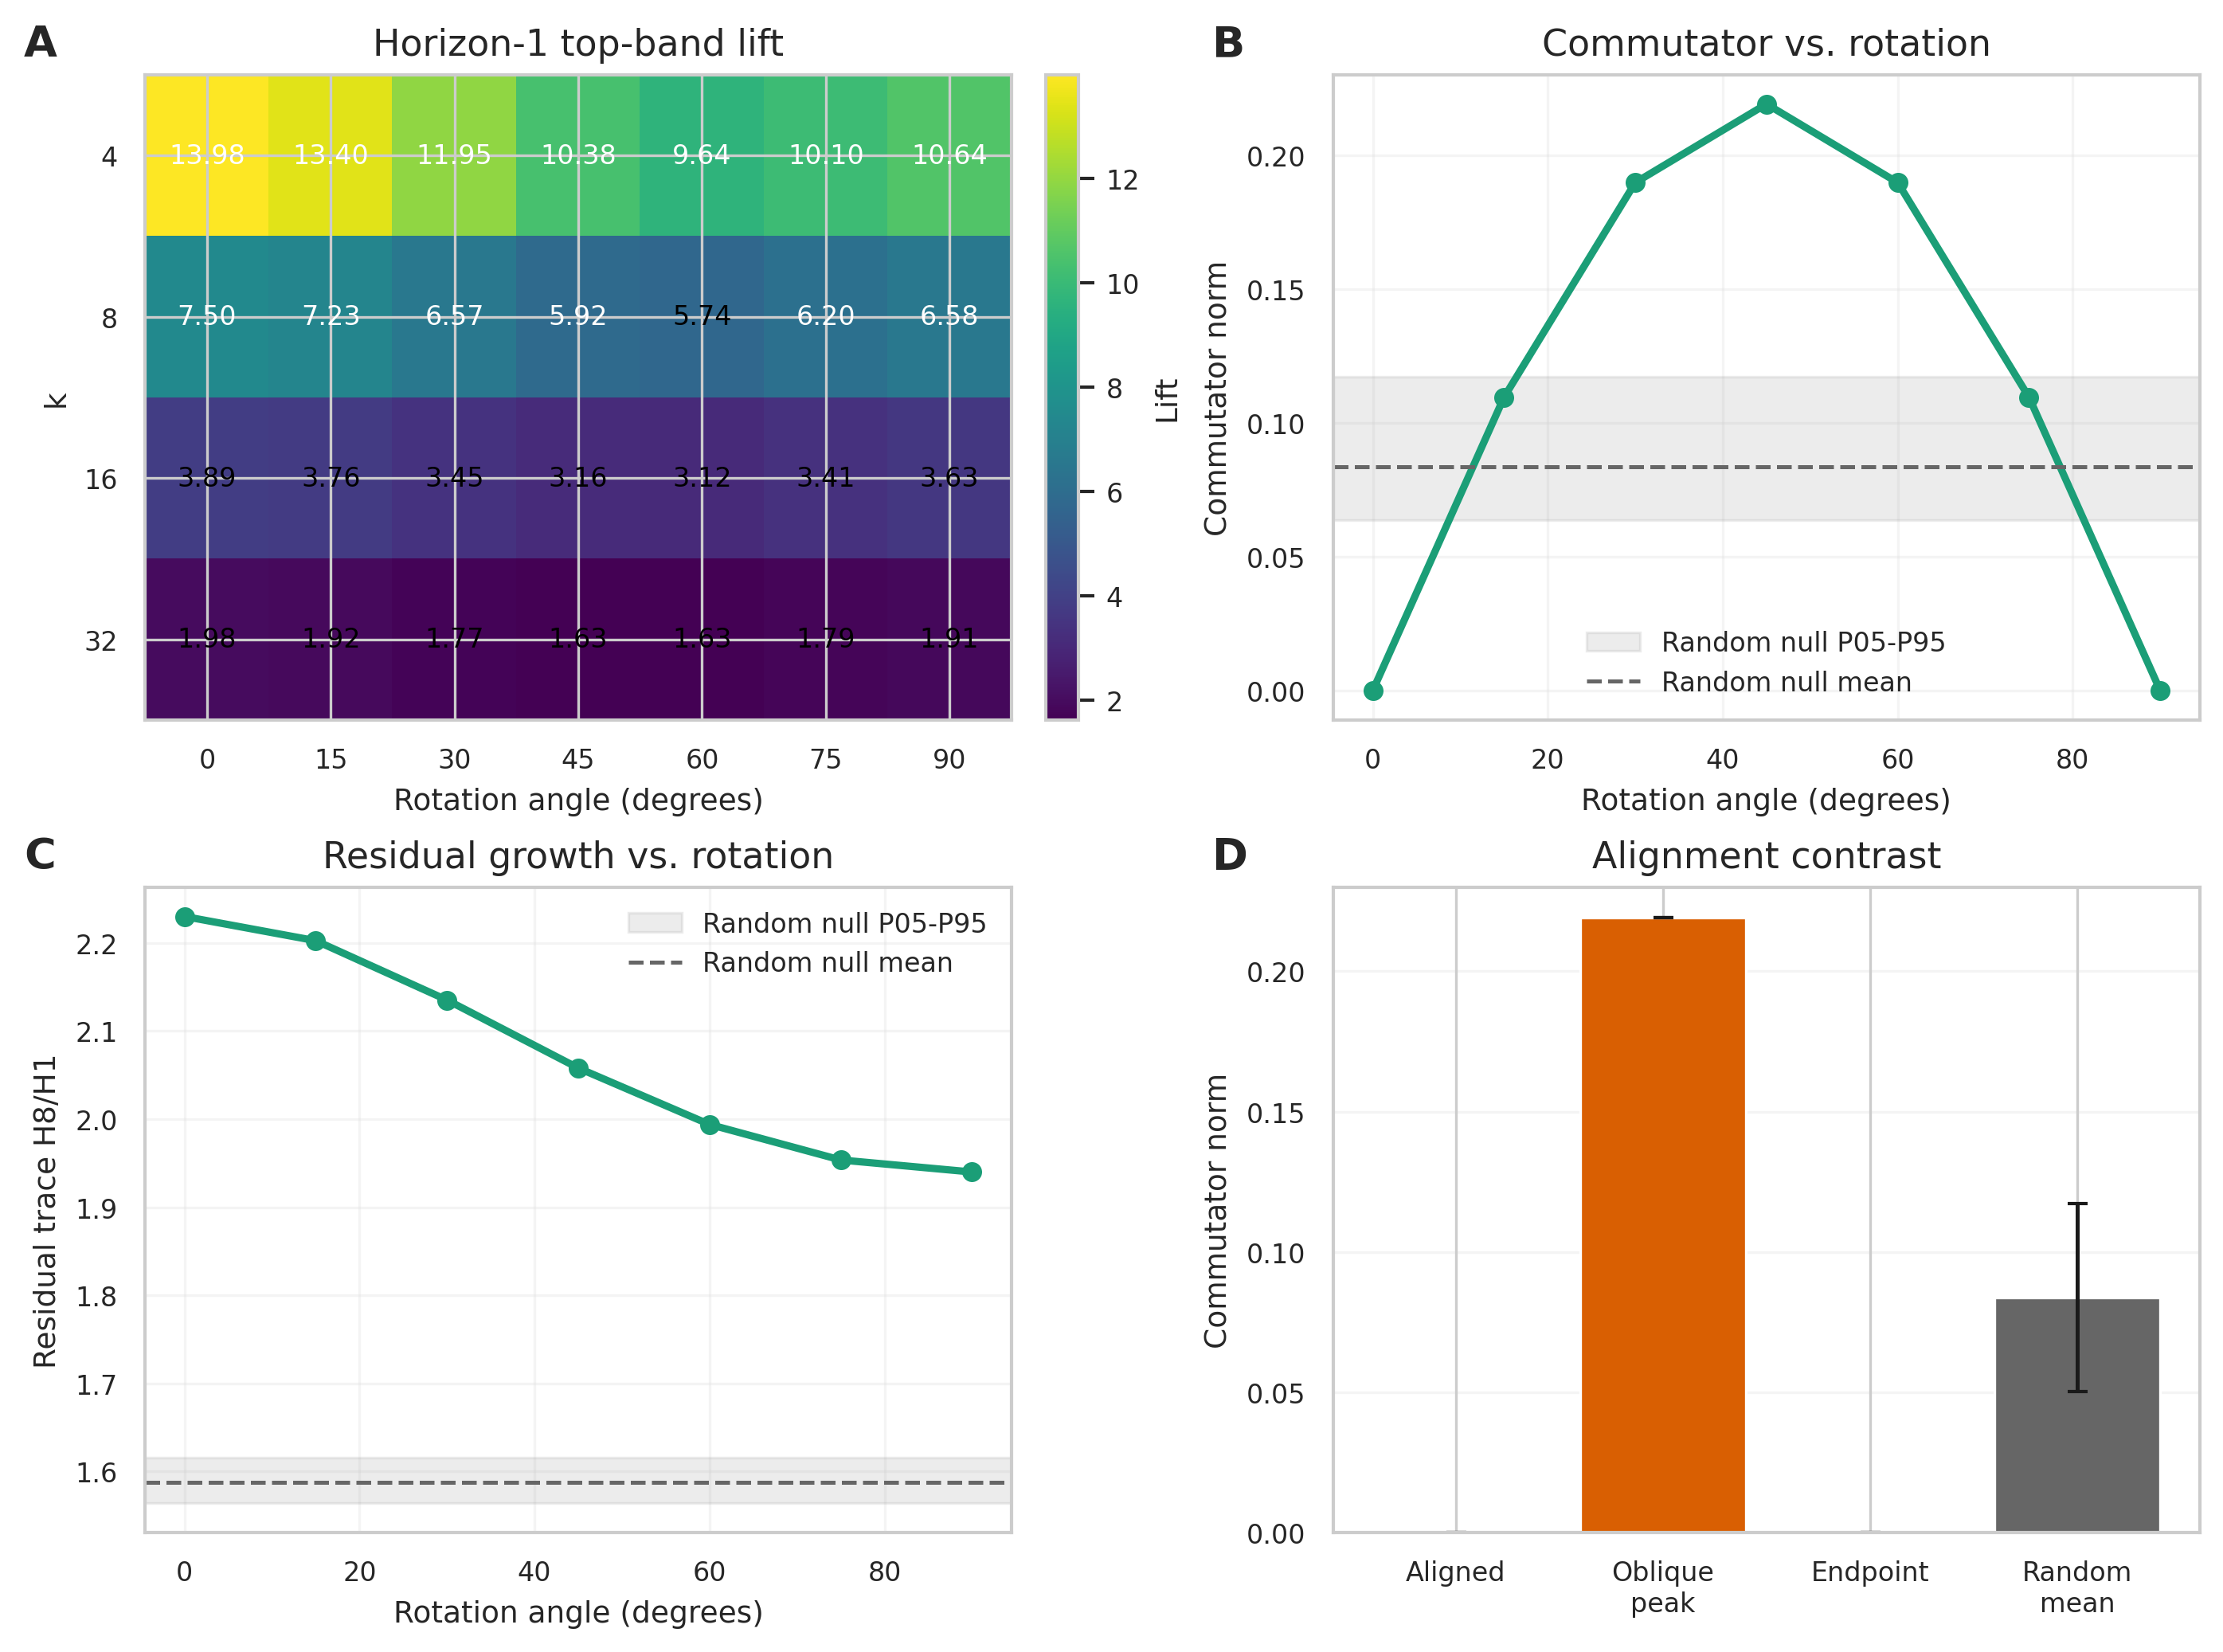
\includegraphics[width=0.74\linewidth]{figures/operator_alignment_summary.png}
  \caption{Main commutator and eigenspace-alignment figure. The same-spectrum rotation changes commutator, top-band lift, and residual growth.}
  \label{fig:supp-main}
\end{figure}

\section{Null Comparisons}
\label{sec:supp-null}

The null suite distinguishes the proposed commutator identity from two nearby explanations. The permutation-preserving null keeps the pair jointly diagonal, so it tests whether coordinate reordering alone can create the signal. The random-basis null keeps the predictor spectrum but removes the structured single-plane perturbation, so it tests whether any spectrum-matched basis is sufficient.

\begin{table}[H]
\centering
\caption{Spectrum-preserving null sweep. The oblique construction is compared with a jointly diagonal permutation control and a spectrum-matched random-basis control. Larger $\mathcal C$ indicates greater covariance--predictor eigenspace mismatch.}
\label{tab:supp-null}
\begin{tabular*}{\linewidth}{@{\extracolsep{\fill}}lrrr@{}}
\toprule
Basis construction & Mean $\mathcal C$ & 5th percentile & 95th percentile \\
\midrule
Oblique plane rotation & 0.219063 & 0.219063 & 0.219063 \\
Permutation-preserving null & 0.000000 & 0.000000 & 0.000000 \\
Random-basis null & 0.084512 & 0.061633 & 0.121488 \\
\bottomrule
\end{tabular*}
\end{table}

The random-basis distribution from the main sweep has commutator mean
$0.0836631$ and a 5th--95th percentile interval of $[0.0637529,0.11723]$;
its residual-growth and predicted-decay means are $1.58794$ and $0.211866$.
These controls are intentionally nonzero. Random bases can create
noncommutativity, but they do not reproduce the structured peak generated by
the single-plane rotation.

\section{Factor-Isolating Ablations}
\label{sec:supp-ablation}

The main ablation separates two variables that a spectrum-only summary would conflate. The first block fixes spectrum and varies alignment. The second fixes alignment at $45^\circ$ and varies input spectral anisotropy. This establishes that spectrum shape affects effect size, while basis alignment remains an independent descriptor of covariance-predictor action.

\begin{table}[H]
\centering
\caption{Decoupling predictor spectrum from covariance--predictor eigenspace alignment. The two blocks vary one factor while holding the other fixed.}
\label{tab:supp-decoupling}
\setlength{\tabcolsep}{3pt}
\begin{tabular*}{\linewidth}{@{\extracolsep{\fill}}llrrrr@{}}
\toprule
Isolation axis & Perturbation & \shortstack{Latent\\stable rank} & \shortstack{Normalized\\commutator $\mathcal C$} & \shortstack{$h=1$\\top-band lift} & \shortstack{Residual ratio\\$\mathcal E_8/\mathcal E_1$} \\
\midrule
Fixed spectrum & $0^\circ$ angle & 4.74389 & 0.000000 & 1.98127 & 2.23004 \\
Fixed spectrum & $45^\circ$ angle & 4.74389 & 0.219063 & 1.63077 & 2.05798 \\
Fixed spectrum & $90^\circ$ angle & 4.74389 & 0.000000 & 1.90720 & 1.93994 \\
\midrule
Fixed alignment & exponent 0.0 & 14.60210 & 0.114121 & 1.65769 & 1.78340 \\
Fixed alignment & exponent 0.5 & 7.89448 & 0.176617 & 1.65943 & 1.91872 \\
Fixed alignment & exponent 1.0 & 4.74389 & 0.219063 & 1.63077 & 2.05798 \\
Fixed alignment & exponent 1.5 & 3.18365 & 0.244025 & 1.58815 & 2.16180 \\
Fixed alignment & exponent 2.0 & 2.36335 & 0.258604 & 1.54226 & 2.19337 \\
\bottomrule
\end{tabular*}
\end{table}

\begin{table}[H]
\centering
\setlength{\tabcolsep}{3pt}
\caption{Robustness of transfer readouts to the chosen energy band and horizon. The same rotation grid is evaluated with four readouts.}
\label{tab:supp-metric}
\begin{tabular*}{\linewidth}{@{\extracolsep{\fill}}lrrrr@{}}
\toprule
Rotation angle & \shortstack{$h=1$\\top-band lift} & \shortstack{$h=1$\\residual-band lift} & \shortstack{$h=8$\\top-band lift} & \shortstack{$h=8$\\residual-band lift} \\
\midrule
$0^\circ$ & 1.98127 & 1.39623 & 2.00000 & 1.62670 \\
$15^\circ$ & 1.91896 & 1.35963 & 1.86631 & 1.60092 \\
$30^\circ$ & 1.76871 & 1.30747 & 1.50133 & 1.55792 \\
$45^\circ$ & 1.63077 & 1.32836 & 1.00394 & 1.55638 \\
$60^\circ$ & 1.62753 & 1.43086 & 0.511423 & 1.61080 \\
$75^\circ$ & 1.78847 & 1.54632 & 0.178818 & 1.68093 \\
$90^\circ$ & 1.90720 & 1.59578 & 0.227794 & 1.71232 \\
\bottomrule
\end{tabular*}
\end{table}

\section{Anisotropy and Dimension Boundaries}
\label{sec:supp-boundary}

The anisotropy scan changes the input spectral exponent continuously while holding the oblique angle fixed. The peak angle remains $45^\circ$ in the tested grid, while peak commutator grows as stable rank decreases.

\begin{table}[H]
\centering
\caption{Continuous sweep over input spectral anisotropy.}
\label{tab:supp-anisotropy}
\begin{tabular*}{0.84\linewidth}{@{\extracolsep{\fill}}rrrr@{}}
\toprule
Input exponent & \shortstack{Latent\\stable rank} & \shortstack{Peak normalized\\commutator $\mathcal C$} & \shortstack{Peak\\top-band lift} \\
\midrule
0.0 & 14.60210 & 0.114121 & 1.00506 \\
0.5 & 7.89448 & 0.176617 & 1.00457 \\
1.0 & 4.74389 & 0.219063 & 1.00394 \\
1.5 & 3.18365 & 0.244025 & 1.00334 \\
2.0 & 2.36335 & 0.258604 & 1.00281 \\
\bottomrule
\end{tabular*}
\end{table}

\begin{table}[H]
\centering
\caption{Cross-dimension theory sweep. The ordering induced by predictor spectral decay is evaluated at three finite dimensions.}
\label{tab:supp-dimension}
\setlength{\tabcolsep}{2.5pt}
\begin{tabular*}{\linewidth}{@{\extracolsep{\fill}}rrrrlrr@{}}
\toprule
Dimension & \shortstack{Baseline\\$\mathcal E_8/\mathcal E_1$} & \shortstack{$\beta=0.5$\\$\mathcal E_8/\mathcal E_1$} & \shortstack{$\beta=2.0$\\$\mathcal E_8/\mathcal E_1$} & \shortstack{Ordering\\preserved?} & \shortstack{Tail\\gap} & \shortstack{Heat-recovery\\$R^2$} \\
\midrule
64 & 2.23004 & 4.56383 & 1.39186 & Yes & 1.0 & 0.999922 \\
128 & 1.98384 & 3.85419 & 1.31785 & Yes & 1.0 & 0.999977 \\
256 & 1.81068 & 3.34861 & 1.26605 & Yes & 1.0 & 0.999953 \\
\bottomrule
\end{tabular*}
\end{table}

\section{Mechanism Sweep}
\label{sec:supp-mechanism}

The mechanism sweep tests how residual growth changes when the analytical generator varies encoder and predictor spectral response. It reports residual growth, predicted decay, and tail-band residual concentration under the same deterministic construction used by the main experiments.

\begin{table}[H]
\centering
\caption{Interaction between encoder and predictor spectral response. Each row reports the resulting residual growth and predicted-trace ratio.}
\label{tab:supp-interaction}
\setlength{\tabcolsep}{3pt}
\begin{tabular*}{\linewidth}{@{\extracolsep{\fill}}rrrrr@{}}
\toprule
\shortstack{Encoder\\exponent} & \shortstack{Predictor\\exponent} & \shortstack{Latent spectral\\exponent} & \shortstack{Residual ratio\\$\mathcal E_8/\mathcal E_1$} & \shortstack{Predicted-trace ratio\\$\mathcal P_8/\mathcal P_1$} \\
\midrule
0.5 & 0.5 & 0.75 & 3.33115 & 0.231924 \\
0.5 & 1.0 & 0.75 & 1.73926 & 0.306679 \\
0.5 & 2.0 & 0.75 & 1.21394 & 0.520081 \\
1.0 & 0.5 & 1.00 & 3.85419 & 0.352804 \\
1.0 & 1.0 & 1.00 & 1.98384 & 0.425678 \\
1.0 & 2.0 & 1.00 & 1.31785 & 0.612044 \\
1.5 & 0.5 & 1.25 & 4.58154 & 0.475850 \\
1.5 & 1.0 & 1.25 & 2.32305 & 0.534648 \\
1.5 & 2.0 & 1.25 & 1.45725 & 0.686855 \\
2.0 & 0.5 & 1.50 & 5.53159 & 0.584591 \\
2.0 & 1.0 & 1.50 & 2.75917 & 0.626212 \\
2.0 & 2.0 & 1.50 & 1.62741 & 0.746749 \\
\bottomrule
\end{tabular*}
\end{table}

\begin{table}[H]
\centering
\setlength{\tabcolsep}{3pt}
\caption{Sensitivity to the synthetic heat filter. The table reports retained trace, tail-band mass, and recovery of the known generator.}
\label{tab:supp-heat}
\begin{tabular*}{\linewidth}{@{\extracolsep{\fill}}rrrrr@{}}
\toprule
\shortstack{Heat\\exponent} & \shortstack{Diffusion\\time} & \shortstack{Retained\\trace fraction} & \shortstack{Retained\\tail fraction} & \shortstack{Generator-recovery\\$R^2$} \\
\midrule
0.5 & 0.000 & 1.000000 & 0.126861 & 0.960860 \\
0.5 & 0.001 & 0.992239 & 0.125425 & 0.960860 \\
0.5 & 0.003 & 0.976993 & 0.122591 & 0.960860 \\
0.5 & 0.010 & 0.926403 & 0.113063 & 0.960860 \\
0.5 & 0.030 & 0.802470 & 0.089073 & 0.960860 \\
1.0 & 0.000 & 1.000000 & 0.126861 & 0.999792 \\
1.0 & 0.001 & 0.955755 & 0.110312 & 0.999792 \\
1.0 & 0.003 & 0.881913 & 0.082903 & 0.999792 \\
1.0 & 0.010 & 0.717684 & 0.029450 & 0.999792 \\
1.0 & 0.030 & 0.523308 & 0.001538 & 0.999792 \\
2.0 & 0.000 & 1.000000 & 0.126861 & 0.127313 \\
2.0 & 0.001 & 0.625067 & 0.000004 & 0.127313 \\
2.0 & 0.003 & 0.524025 & 0.000000 & 0.127313 \\
2.0 & 0.010 & 0.413441 & 0.000000 & 0.127313 \\
2.0 & 0.030 & 0.312955 & 0.000000 & 0.127313 \\
\bottomrule
\end{tabular*}
\end{table}

\begin{table}[H]
\centering
\setlength{\tabcolsep}{3pt}
\caption{Oblique-frame stress test. Increasing obliqueness changes finite-window slope bias and the frame condition number.}
\label{tab:supp-oblique}
\begin{tabular*}{\linewidth}{@{\extracolsep{\fill}}rrrr@{}}
\toprule
Obliqueness & \shortstack{Baseline mean\\absolute bias} & \shortstack{Broken-tail mean\\absolute bias} & \shortstack{Frame condition\\number} \\
\midrule
0.00 & 0.000000 & 0.000000 & 1.00000 \\
0.25 & 0.129676 & 0.072982 & 1.63916 \\
0.50 & 0.415790 & 0.262480 & 2.71704 \\
0.75 & 0.759680 & 0.517336 & 4.54002 \\
1.00 & 1.12440 & 0.810285 & 7.64852 \\
\bottomrule
\end{tabular*}
\end{table}

\section{Robustness Sweeps}
\label{sec:supp-robustness}

The robustness sweep varies random seeds for auxiliary frame diagnostics and adds small perturbations to the heat-recovery experiment. These measurements check whether the reported diagnostic quantities are stable under nuisance variation in the analytical setup.

\begin{table}[H]
\centering
\caption{Seed robustness of oblique-bias and frame diagnostics. Entries summarize nuisance draws in the analytical setup.}
\label{tab:supp-seed-robustness}
\begin{tabular}{lcccc}
\toprule
Diagnostic quantity & Mean & Standard deviation & Minimum & Maximum \\
\midrule
Baseline oblique bias & 0.432336 & 0.009375 & 0.415378 & 0.441991 \\
Broken-tail oblique bias & 0.284172 & 0.011879 & 0.262480 & 0.303541 \\
Frame condition number & 2.61823 & 0.048972 & 2.56380 & 2.71704 \\
\bottomrule
\end{tabular}
\end{table}

\begin{table}[H]
\centering
\caption{Recovery of the known heat generator under additive noise.}
\label{tab:supp-heat-noise}
\begin{tabular}{cccc}
\toprule
Noise standard deviation & Mean $R^2$ & Minimum $R^2$ & Maximum $R^2$ \\
\midrule
0.00 & 1.000000 & 1.000000 & 1.000000 \\
0.01 & 0.999980 & 0.999977 & 0.999983 \\
0.03 & 0.999819 & 0.999790 & 0.999849 \\
0.05 & 0.999498 & 0.999416 & 0.999580 \\
\bottomrule
\end{tabular}
\end{table}

\section{Diagonal-Transfer Spectral Diagnostics}
\label{sec:supp-rich}

This section reports diagonal-transfer diagnostics that complement the same-spectrum construction. The sweep varies predictor decay and broken-tail spectral structure, then reports residual growth, fitted residual decay, and heat-recovery accuracy under the analytical generator.

\begin{table}[H]
\centering
\caption{Diagonal-transfer spectral diagnostics. Rows vary predictor decay or introduce broken-tail spectral structure under the analytical generator.}
\label{tab:supp-earlier}
\small
\setlength{\tabcolsep}{3pt}
\resizebox{\linewidth}{!}{%
\begin{tabular}{@{}p{0.26\linewidth}ccccc@{}}
\toprule
Case & Latent exponent $\alpha$ & Tail gap & Residual exponent & Residual ratio $\mathcal E_8/\mathcal E_1$ & Heat-recovery $R^2$ \\
\midrule
Baseline & 1.00000 & 0.000000 & 0.691532 & 1.98384 & 0.999977 \\
Predictor 0.5 & 1.00000 & 0.000000 & 0.538399 & 3.85419 & 0.999977 \\
Predictor 2.0 & 1.00000 & 0.000000 & 0.861305 & 1.31785 & 0.999977 \\
Broken tail 3 b32 & 1.44847 & 1.00000 & 1.18434 & 2.19174 & 0.999977 \\
Broken tail 4 b64 & 1.25910 & 1.50000 & 0.979362 & 2.06464 & 0.999977 \\
\bottomrule
\end{tabular}
}
\end{table}

\section{Auxiliary Subspace-Rotation Diagnostic}
\label{sec:supp-auxiliary}

This auxiliary sweep checks a second spectrum-fixed rotation diagnostic. It measures how rotating the observed subspace changes latent mass, residual energy, and top-band lift under the same synthetic construction.

\begin{table}[H]
\centering
\caption{Auxiliary subspace-rotation sweep. The spectrum is fixed while the measured subspace is rotated.}
\label{tab:supp-control}
\begin{tabular}{cccc}
\toprule
Rotation angle & Latent-mass share & Residual-energy share & Top-$32$ lift \\
\midrule
$0^\circ$ & 0.572917 & 0.249719 & 2.00000 \\
$15^\circ$ & 0.536409 & 0.283857 & 1.86603 \\
$30^\circ$ & 0.436667 & 0.377125 & 1.50000 \\
$45^\circ$ & 0.300416 & 0.504532 & 1.00000 \\
$60^\circ$ & 0.164165 & 0.631938 & 0.50000 \\
$75^\circ$ & 0.064422 & 0.725206 & 0.133975 \\
$90^\circ$ & 0.027914 & 0.759345 & 0.000000 \\
\bottomrule
\end{tabular}
\end{table}

The random null for this diagnostic has top-$32$ lift mean $1.01115$ with a 5th--95th percentile interval from $0.927697$ to $1.09239$. Its residual-share mean is $0.616699$ and latent-mass-share mean is $0.127282$. The structured rotation therefore changes both top-band mass and residual share relative to the random-subspace reference.

\section{Frozen PushT Latent Measurements}
\label{sec:supp-frozen-pusht}

The theory construction is synthetic by design, but the same measurement vocabulary can be applied to frozen learned latents. This section reports an offline measurement on frozen PushT latents with top-band size $k=32$. The readouts compare observed latent directions with randomized controls that preserve scale or randomize basis structure.

\begin{table}[H]
\centering
\small
\setlength{\tabcolsep}{3pt}
\caption{Frozen PushT top-band readouts. Observed top-$32$ lift is compared with a norm-matched randomized control; ratios above one indicate greater concentration in the top covariance band than in the reference.}
\label{tab:supp-pusht-lift}
\resizebox{\linewidth}{!}{%
\begin{tabular}{lccc}
\toprule
Readout & Observed top-band lift & Randomized-reference lift & Observed/reference ratio \\
\midrule
Dynamics & 4.71084 & 1.00082 & 4.70698 \\
Planner-weighted & 4.62362 & 1.00082 & 4.61983 \\
Predicted dynamics & 4.68678 & 1.00082 & 4.68294 \\
Prediction residual & 3.68668 & 1.00082 & 3.68366 \\
\bottomrule
\end{tabular}
}
\end{table}

\begin{table}[H]
\centering
\small
\setlength{\tabcolsep}{3pt}
\caption{Frozen PushT label-shuffle controls. Shuffles remove action labels, state-cluster labels, or temporal ordering while retaining the same frozen latent records and top-$32$ readout.}
\label{tab:supp-pusht-shuffle}
\resizebox{\linewidth}{!}{%
\begin{tabular}{lcccc}
\toprule
Readout & Observed ordering & Action-label shuffle & State-label shuffle & Temporal-order shuffle \\
\midrule
Dynamics & 4.71084 & 1.86731 & 1.86817 & 2.18068 \\
Planner-weighted & 4.62362 & 1.94846 & 1.94945 & 2.14740 \\
Predicted dynamics & 4.68678 & 1.83563 & 1.83670 & 2.16529 \\
Prediction residual & 3.68668 & 1.96542 & 1.96579 & 2.05093 \\
\bottomrule
\end{tabular}
}
\end{table}

\begin{table}[H]
\centering
\caption{Frozen PushT transition-overlap distribution. Observed transitions are compared with a random-subspace reference using the same top-band size $k=32$.}
\label{tab:supp-pusht-overlap}
\begin{tabular}{lcc}
\toprule
Statistic & Observed transitions & Random-subspace reference \\
\midrule
Mean overlap & 0.029970 & 0.020953 \\
5th-percentile overlap & 0.004339 & 0.010673 \\
95th-percentile overlap & 0.111357 & 0.034016 \\
\bottomrule
\end{tabular}
\end{table}

\begin{table}[H]
\centering
\small
\setlength{\tabcolsep}{3pt}
\caption{Frozen PushT conditioning sweep. The same top-$32$ readouts are recomputed under state-, action-, latent-, and global-conditioned summaries.}
\label{tab:supp-pusht-condition}
\resizebox{\linewidth}{!}{%
\begin{tabular}{lcccc}
\toprule
Conditioning summary & Dynamics & Predicted dynamics & Prediction residual & Planner-weighted dynamics \\
\midrule
States & 4.67541 & 4.64709 & 3.66198 & 4.59063 \\
Actions & 2.83562 & 2.82753 & 2.42784 & 2.97068 \\
Latents & 5.29517 & 5.27070 & 4.00016 & 5.18173 \\
Global & 1.83645 & 1.79945 & 1.95409 & 1.90871 \\
\bottomrule
\end{tabular}
}
\end{table}

To test whether the state-conditioned action readout is an in-sample artifact,
we independently split each of the eight state cells into two halves, fit a
zero-intercept linear map from actions to dynamics on one half, and evaluate it
on the other half. For a test index set $I_{\mathrm{test}}$, the reported score
is
\begin{equation}
R^2_{\mathrm{test}}=1-
\frac{\sum_{i\in I_{\mathrm{test}}}
\lVert \Delta z_i-a_i\widehat B_{\mathrm{train}}\rVert_2^2}
{\sum_{i\in I_{\mathrm{test}}}
\lVert \Delta z_i-\overline{\Delta z}_{\mathrm{test}}\rVert_2^2},
\label{eq:supp-heldout-r2}
\end{equation}
where $\widehat B_{\mathrm{train}}$ is estimated only on the complementary
training half. The permutation null shuffles action rows within the sampled
artifact before applying the same split and estimator.

\begin{table}[H]
\centering
\small
\setlength{\tabcolsep}{3pt}
\caption{State-conditioned action-to-dynamics readout with an independent
held-out and permutation-null check. Each seed uses 20,000 deterministic rows,
eight state cells, and a within-cell half/half split. The primary fit has no
intercept; the score is descriptive and is not a controllability or planning
metric. The final column counts cells whose $k=32$ dynamics-minus-controllable
lift is non-positive.}
\label{tab:supp-pusht-controllability}
\resizebox{\linewidth}{!}{%
\begin{tabular}{lrrrrr}
\toprule
Initialization replicate & Pooled in-sample $R^2$ & Held-out cell $R^2$ mean & Held-out cell range & Permuted-action null & Non-positive cells / 8 \\
\midrule
3072 & 0.03198 & 0.06034 & 0.04524--0.07535 & $-0.02422$ & 8 \\
3073 & 0.03121 & 0.05593 & 0.04449--0.08024 & $-0.03469$ & 8 \\
3074 & 0.03194 & 0.05502 & 0.04194--0.07600 & $-0.03460$ & 8 \\
\bottomrule
\end{tabular}
}
\end{table}

The held-out cell-level scores are positive for all three seeds and exceed the
corresponding action-permutation nulls. The in-sample state-cell means are also
above the pooled in-sample readout, but the held-out check is the more relevant
guard against a same-sample fit artifact. No cell is flagged by the report's
operational high-variance/low-controllability diagnostic, and all 24 cells have
non-positive $k=32$ dynamics-minus-controllable lift. These checks support the
narrow statement that action information is detectable in the frozen latent
dynamics under state conditioning. They do not establish a causal
controllability mechanism, goal reachability, physical observability, online
planning, or multi-step rollout quality; the export lacks goals, success,
episode/timestep identifiers, physical variables, counterfactual transitions,
and multi-horizon dynamics.

These learned-latent measurements show that basis-sensitive statistics move
relative to randomized controls. The mean transition overlap is $1.43\times$
the random-subspace mean, the observed upper tail is wider than the null
interval, and planner weights put $1.44\times$ more mass on the top latent band
than on the tail band. Recomputing the state-conditioned readouts on the two
stored sample sizes changes the dynamics lift from $4.67541$ to $4.71084$;
the corresponding ratios for predicted dynamics, residual, and planner-weighted
readouts are $0.99153$, $0.99330$, and $0.99287$. The stable ordering across
these records indicates that the readout is not determined by a single sample
cap, while the absolute value remains a property of the sampling protocol.

The PushT measurements show that the alignment-sensitive readouts are nontrivial
in frozen learned latents. Because the stored records support offline one-step
analysis, these results characterize representation geometry rather than online
rollouts, counterfactual transitions, or task success.

\section{Alignment Interventions and Prediction Boundaries}
\label{sec:supp-intervention}

The diagnostic is not itself a claim that lower covariance--predictor mismatch
must improve prediction. We therefore add two matched intervention studies.
The first is a learned synthetic benchmark in which two action groups have
different covariance and transition spectra. Each local covariance--transition
pair commutes (the exact local normalized commutators are $0$ and
$5.68\times10^{-16}$), whereas the pooled data-generating commutator is
$0.354281$. An identical action-conditioned linear predictor is trained with
no alignment, global alignment, or action-conditional alignment. All rows use
the same generated splits, initialization seeds, optimizer, and 300-epoch
training protocol. The rollout metric repeats each sample's action label at
every step, so it is a repeated-action stability diagnostic rather than an
arbitrary action-sequence evaluation. Ordered two-action composition is
measured separately for $0\!\to\!0$, $0\!\to\!1$, $1\!\to\!0$, and
$1\!\to\!1$.

\begin{table}[H]
\centering
\small
\setlength{\tabcolsep}{3pt}
\caption{Learned synthetic intervention matrix. The local data-generating
operators commute, but the pooled geometry is heterogeneous. Values are means
over three seeds; the one-step MSE and $h=8$ rollout MSE are evaluated on a
held-out split and the rollout repeats the same action label. Composition error
is the mean normalized error over the four ordered two-action products. The
experiment is a mechanism boundary test, not a learned LeWorldModel result.}
\label{tab:supp-synthetic-intervention}
\resizebox{\linewidth}{!}{%
\begin{tabular}{llrrrrr}
\toprule
Mode & Weight & Test one-step MSE & $h=8$ rollout MSE & Composition error & Global $\mathcal C$ & Conditional $\mathcal C$ \\
\midrule
None & 0 & $2.45792\times10^{-6}$ & $1.93476\times10^{-6}$ & 0.00815304 & 0.355696 & $3.22857\times10^{-5}$ \\
Global & 0.01 & $2.19856\times10^{-5}$ & $1.78173\times10^{-5}$ & 0.0146905 & 0.351926 & $5.84717\times10^{-5}$ \\
Global & 0.1 & $3.98326\times10^{-3}$ & $4.30374\times10^{-3}$ & 0.361108 & 0.288497 & $2.25252\times10^{-3}$ \\
Global & 1 & $8.07862\times10^{-2}$ & $3.80981\times10^{1}$ & 3.78536 & 0.0740325 & 0.019993 \\
Global & 10 & 0.290907 & 0.509461 & 1.63435 & 0.0033793 & 0.295549 \\
Global & 100 & 0.350466 & 0.492963 & 1.38404 & 0.000430968 & 0.269849 \\
Conditional & 0.01 & $2.24614\times10^{-6}$ & $1.73940\times10^{-6}$ & 0.00756084 & 0.355684 & $2.65222\times10^{-5}$ \\
Conditional & 0.1 & $2.35859\times10^{-6}$ & $1.59203\times10^{-6}$ & 0.00790262 & 0.355676 & $3.15303\times10^{-5}$ \\
Conditional & 1 & $8.22803\times10^{-6}$ & $4.99238\times10^{-6}$ & 0.00913680 & 0.355836 & $4.59051\times10^{-5}$ \\
Conditional & 10 & $2.14002\times10^{-3}$ & $9.13679\times10^{-5}$ & 0.149069 & 0.351436 & $6.80257\times10^{-5}$ \\
Conditional & 100 & 0.0575382 & 0.0205186 & 1.51700 & 0.265642 & $1.72814\times10^{-4}$ \\
\bottomrule
\end{tabular}
}
\end{table}

The synthetic matrix establishes a necessary boundary for interpreting the
regularizer. Conditional alignment preserves the local commutator at small
weight and remains close to the no-alignment predictor, whereas global
alignment imposes an inappropriate pooled geometry and degrades prediction.
At larger conditional weights, the alignment diagnostic can continue to fall
while prediction error rises. Thus commutator reduction is an intervention
target, not a sufficient objective for predictive quality.

We next test the same distinction on real PushT records exported from a frozen
LeWorldModel checkpoint. This is a post-hoc latent adapter rather than
end-to-end retraining. Given the frozen displacement $\widehat{\Delta z}$, the
adapter predicts
\begin{equation}
\widehat z_{t+1}^{\,\mathrm{adapt}} = z_t + \widehat{\Delta z}_{t+1} + g_\phi\!\left(z_t,\widehat{\Delta z}_{t+1},a_t\right),
\label{eq:supp-latent-adapter}
\end{equation}
where $g_\phi$ is initialized at zero and is trained against the exported
one-step displacement. The experiment uses 100,000 deterministic rows, an
80/10/10 row-level split, ten epochs, and three initialization seeds. Because
the compact export does not contain episode or timestep identifiers, only
held-out one-step prediction is evaluated.

\begin{table}[H]
\centering
\small
\setlength{\tabcolsep}{3pt}
\caption{Frozen PushT latent-adapter intervention. The frozen row is the
released predictor without an adapter; all other rows are the same learned
residual adapter with the indicated alignment penalty. Paired MSE deltas are
computed within seed relative to the no-alignment adapter.}
\label{tab:supp-real-intervention}
\resizebox{\linewidth}{!}{%
\begin{tabular}{lrrrr}
\toprule
Intervention & Weight & Held-out MSE & Paired $\Delta$MSE vs. none & Conditional $\mathcal C$ \\
\midrule
Frozen predictor & -- & 0.00776849 & -- & 0.00921481 \\
Adapter, none & 0 & 0.00622429 & 0 & 0.00913191 \\
Adapter, global & 0.001 & 0.00622426 & $-2.28\times10^{-8}$ & 0.00913102 \\
Adapter, global & 0.01 & 0.00622410 & $-1.89\times10^{-7}$ & 0.00912299 \\
Adapter, global & 0.1 & 0.00622562 & $+1.33\times10^{-6}$ & 0.00904336 \\
Adapter, conditional & 0.001 & 0.00622427 & $-1.37\times10^{-8}$ & 0.00913080 \\
Adapter, conditional & 0.01 & 0.00622419 & $-9.86\times10^{-8}$ & 0.00912071 \\
Adapter, conditional & 0.1 & 0.00622677 & $+2.48\times10^{-6}$ & 0.00902090 \\
\bottomrule
\end{tabular}
}
\end{table}

The residual adapter itself supplies the main one-step improvement over the
frozen predictor. Relative to that matched adapter baseline, alignment changes
the conditional diagnostic but has only a negligible effect at weight $0.01$;
the stronger conditional penalty lowers $\mathcal C$ further while worsening
MSE. These real-record results therefore support a narrower conclusion:
alignment is an identifiable intervention on the latent geometry, but its
predictive value is conditional on the weighting and cannot be inferred from
the diagnostic alone. They do not establish end-to-end training gains,
multi-step rollout gains, or online planning success.

\subsection{External Multi-step Adapter and Normalization Robustness}
\label{sec:supp-external-adapter-robustness}

The preceding row-level adapter does not test whether a geometry intervention
survives autoregressive rollout. We therefore fit a second, deliberately small
residual adapter on one-step transitions from the public external PushT
archive and evaluate it on held-out episodes. The LeWorldModel encoder and
predictor remain frozen. There are 21 episodes and 42 windows; three episode
split seeds ($3072$--$3074$) and three adapter initialization seeds are used.
The alignment weights are $0.01$, $0.1$, and $1.0$, and the two modes are the
global and action-conditional penalties. The public action normalization is
repeated with validation-split $z$-scoring and raw actions divided by $100$.
All conditions use the same checkpoint-selection rule and held-out rollout
code. The independent unit is the episode split seed, with initialization
seeds nested inside it.

Table~\ref{tab:supp-external-adapter-h8} reports the primary $h=8$ contrast,
defined as adapted minus matched no-alignment rollout MSE. Negative values
favor the adapter. The public-normalization global condition is consistently
positive at $h=8$, whereas the conditional condition is mostly compatible
with zero. Under the other normalizations, signs and magnitudes change with
the penalty weight. Thus a measurable alignment intervention does not imply a
monotone multi-step gain.

\begin{table}[H]
\centering
\scriptsize
\setlength{\tabcolsep}{3pt}
\caption{External frozen temporal adapter robustness at $h=8$. Values are
split-level paired MSE deltas (adapter minus no-alignment) with 95\% episode
bootstrap intervals. Negative values favor the adapter.}
\label{tab:supp-external-adapter-h8}
\resizebox{\linewidth}{!}{%
\begin{tabular}{lllrr}
\toprule
Normalization & Mode & Weight & $\Delta$MSE vs.~none & 95\% interval \\
\midrule
public & global & 0.01 & $+0.006871$ & $[+0.000046,+0.020366]$ \\
public & global & 0.1 & $+0.007218$ & $[+0.003033,+0.014978]$ \\
public & global & 1 & $+0.027554$ & $[+0.001312,+0.075299]$ \\
public & conditional & 0.01 & $+0.000450$ & $[-0.000146,+0.001206]$ \\
public & conditional & 0.1 & $+0.002983$ & $[-0.002650,+0.006824]$ \\
public & conditional & 1 & $+0.003585$ & $[-0.011599,+0.026681]$ \\
validation $z$-score & global & 0.01 & $-0.000079$ & $[-0.000824,+0.000586]$ \\
validation $z$-score & global & 0.1 & $-0.000847$ & $[-0.006940,+0.002486]$ \\
validation $z$-score & global & 1 & $-0.005210$ & $[-0.022712,+0.007698]$ \\
validation $z$-score & conditional & 0.01 & $+0.000169$ & $[-0.001300,+0.001603]$ \\
validation $z$-score & conditional & 0.1 & $+0.000895$ & $[-0.008999,+0.009866]$ \\
validation $z$-score & conditional & 1 & $-0.037889$ & $[-0.123547,+0.038389]$ \\
raw$/100$ & global & 0.01 & $+0.000122$ & $[+0.000046,+0.000202]$ \\
raw$/100$ & global & 0.1 & $+0.000155$ & $[-0.000530,+0.000957]$ \\
raw$/100$ & global & 1 & $+0.000553$ & $[-0.002457,+0.004996]$ \\
raw$/100$ & conditional & 0.01 & $+0.000219$ & $[+0.000123,+0.000312]$ \\
raw$/100$ & conditional & 0.1 & $+0.000727$ & $[+0.000207,+0.001428]$ \\
raw$/100$ & conditional & 1 & $+0.003174$ & $[-0.001608,+0.008897]$ \\
\bottomrule
\end{tabular}
}
\end{table}

\subsection{Temporal Directionality and Lag Controls}
\label{sec:supp-temporal-directionality}

To test whether the transferred dynamics-sensitive subspace contains more
than static state or smooth action information, we performed a separate
episode-level leave-one-out audit. For each external window and horizon $h$,
the target is the true encoded latent increment in a source-fitted basis band.
The feature arms are a future-action summary aligned with that increment, a
same-length action summary shifted back by one latent step, the current latent
state, and the corresponding state-augmented action features. A within-episode
derangement swaps the two action sources while preserving their marginal
distribution. The primary contrast is
\begin{equation}
\Delta_{b,h}^{\mathrm{future-past}}
=R^2(\mathrm{future\ action}+\mathrm{state})
-R^2(\mathrm{past\ action}+\mathrm{state}),
\label{eq:supp-temporal-directionality}
\end{equation}
and a second contrast compares future-action $R^2$ with the deranged-action
control. Inference uses episode-cluster bootstrap intervals; no external
window is treated as an independent episode.

The transferred dynamics basis results are shown in
Table~\ref{tab:supp-temporal-directionality}. A cell is counted as supported
only when both 95\% lower bounds (future versus past and future versus
deranged) are positive. None of the 36 cells across the two basis bands,
three horizons, and three normalizations satisfies this strict criterion;
21 cells have positive point estimates for both contrasts, while 15 do not.
The directionality audit therefore rules out a stronger normalization-
invariant temporal-action claim on this external sample. It does not negate
the separate held-out evidence that a dynamics-sensitive subspace can be
extracted or that its coordinates affect frozen rollout error.

\begin{table}[H]
\centering
\scriptsize
\setlength{\tabcolsep}{3pt}
\caption{Temporal directionality controls for the transferred dynamics basis.
Entries are future-plus-state minus past-plus-state $R^2$, followed by
future-action minus deranged-action $R^2$; intervals are 95\% episode
bootstrap intervals.}
\label{tab:supp-temporal-directionality}
\resizebox{\linewidth}{!}{%
\begin{tabular}{llrcc}
\toprule
Normalization & Band & $h$ & $\Delta^{\mathrm{future-past}}$ & $\Delta^{\mathrm{future-deranged}}$ \\
\midrule
public & top-8 & 1 & $-0.0345\ [-0.1301,0.0638]$ & $+0.1465\ [-0.0439,0.2522]$ \\
public & top-8 & 4 & $+0.0084\ [-0.0925,0.1304]$ & $+0.1687\ [-0.0570,0.4288]$ \\
public & top-8 & 8 & $-0.0208\ [-0.1601,0.1467]$ & $+0.0855\ [-0.0439,0.2194]$ \\
public & middle-8--32 & 1 & $+0.4477\ [+0.1260,+0.8129]$ & $+0.1436\ [-0.0189,+0.3490]$ \\
public & middle-8--32 & 4 & $+0.1050\ [-0.1328,+0.3587]$ & $+0.0864\ [-0.0479,+0.2390]$ \\
public & middle-8--32 & 8 & $+0.1007\ [-0.0848,+0.2776]$ & $+0.1106\ [-0.0033,+0.2432]$ \\
validation $z$-score & top-8 & 1 & $-0.0345\ [-0.1300,0.0638]$ & $+0.1465\ [-0.0439,+0.2522]$ \\
validation $z$-score & top-8 & 4 & $+0.0101\ [-0.0936,+0.1358]$ & $+0.1687\ [-0.0570,+0.4287]$ \\
validation $z$-score & top-8 & 8 & $-0.0206\ [-0.1606,+0.1482]$ & $+0.0855\ [-0.0439,+0.2194]$ \\
validation $z$-score & middle-8--32 & 1 & $+0.4475\ [+0.1271,+0.8125]$ & $+0.1436\ [-0.0189,+0.3489]$ \\
validation $z$-score & middle-8--32 & 4 & $+0.0997\ [-0.1615,+0.3762]$ & $+0.0864\ [-0.0479,+0.2389]$ \\
validation $z$-score & middle-8--32 & 8 & $+0.1087\ [-0.0938,+0.2975]$ & $+0.1106\ [-0.0033,+0.2432]$ \\
raw$/100$ & top-8 & 1 & $-0.0342\ [-0.1290,0.0635]$ & $+0.1465\ [-0.0439,+0.2522]$ \\
raw$/100$ & top-8 & 4 & $-0.0129\ [-0.0687,0.0421]$ & $+0.1687\ [-0.0570,+0.4287]$ \\
raw$/100$ & top-8 & 8 & $-0.0239\ [-0.1291,0.1063]$ & $+0.0855\ [-0.0439,+0.2194]$ \\
raw$/100$ & middle-8--32 & 1 & $+0.4269\ [+0.1310,+0.7684]$ & $+0.1436\ [-0.0189,+0.3489]$ \\
raw$/100$ & middle-8--32 & 4 & $+0.0788\ [-0.0036,+0.1601]$ & $+0.0864\ [-0.0479,+0.2390]$ \\
raw$/100$ & middle-8--32 & 8 & $+0.0846\ [-0.0145,+0.1845]$ & $+0.1106\ [-0.0033,+0.2432]$ \\
\bottomrule
\end{tabular}
}
\end{table}

This control is deliberately stronger than a nonzero-action versus zero-action
comparison, but it remains a predictive temporal diagnostic. A positive
future-minus-past contrast would indicate temporal precedence in the encoded
readout, not a counterfactual action effect or physical controllability.

\subsection{Pixel-to-Latent Intervention with a Learned Encoder}
\label{sec:supp-pixel-intervention}

The frozen-adapter study leaves open whether the same boundary is visible when
the representation itself is learned. We therefore repeat the intervention in
a small action-conditioned pixel world. A convolutional encoder and latent
predictor are trained jointly from $16\times16$ torus images using
next-embedding prediction plus SIGReg. Horizontal actions translate by one
pixel and vertical actions by two pixels; the one-step training split includes
a fixed action-group-specific scene offset, while the rollout split uses
random action sequences with exact torus ground truth. All conditions use the
same generated splits, initialization seeds, optimizer, early-stopping rule,
and evaluation code. The result is a learned-encoder diagnostic, not an
end-to-end LeWorldModel or PushT experiment.

\begin{table}[H]
\centering
\small
\setlength{\tabcolsep}{3pt}
\caption{Pixel-to-latent alignment intervention in a synthetic torus world.
The encoder and action-conditioned predictor are trained jointly; entries are
means over three seeds. One-step and $h=8$ rollout MSE are held-out latent
prediction errors, and composition error averages the 16 ordered two-action
products. The two commutators are diagnostics of the learned latent geometry,
not task-performance measures.}
\label{tab:supp-pixel-intervention}
\resizebox{\linewidth}{!}{%
\begin{tabular}{llrrrrrr}
\toprule
Mode & Weight & One-step MSE & $h=8$ rollout MSE & Composition error & Global $\mathcal C$ & Conditional $\mathcal C$ & Stable rank \\
\midrule
None & 0 & 0.000253 & 0.000262 & 1.25651 & 0.183362 & 0.252623 & 2.00777 \\
Global & 0.01 & 0.000549 & 0.000555 & 1.62688 & 0.064230 & 0.108349 & 2.19314 \\
Global & 0.1 & 0.002047 & 0.002004 & 2.40440 & 0.038367 & 0.046918 & 3.42851 \\
Global & 1 & 0.012705 & 0.013520 & 1.96097 & 0.100343 & 0.084603 & 2.79232 \\
Conditional & 0.01 & 0.000393 & 0.000421 & 1.59206 & 0.019057 & 0.013691 & 1.89100 \\
Conditional & 0.1 & 0.001638 & 0.001729 & 1.93547 & 0.027033 & 0.046022 & 2.78120 \\
Conditional & 1 & 0.013387 & 0.014319 & 2.12862 & 0.030234 & 0.021923 & 2.44613 \\
\bottomrule
\end{tabular}
}
\end{table}

Table~\ref{tab:supp-pixel-intervention} reproduces the qualitative boundary
from the linear benchmark after introducing a trainable pixel encoder. The
conditional penalty at weight $0.01$ reduces the conditional commutator from
$0.252623$ to $0.013691$, while one-step MSE, rollout MSE, and composition
error all increase relative to the unregularized model. Global alignment at
weight $0.1$ similarly lowers the pooled commutator to $0.038367$ while
increasing one-step MSE by roughly an order of magnitude and producing the
largest composition error. The learned pixel benchmark therefore supports a
more precise intervention claim: alignment penalties can move conditional
geometry in a trainable representation, but commutator reduction alone does
not imply improved prediction, composition, or rollout stability. Because the
world is synthetic and the encoder is intentionally small, this result does
not support claims about nonlinear LeWorldModel training, PushT performance,
online planning, causal controllability, or GPU efficiency.

\subsection{Latent and Predictor Equivariance in a Controlled Vector World}
\label{sec:supp-equivariance-intervention}

The preceding experiments target covariance--predictor alignment without
assuming a group action. To isolate a complementary question, we construct a
controlled action-conditioned vector world whose transition is
$s_{t+1}=s_t+a_t$. States and actions are four-dimensional vectors made of two
two-dimensional rotation blocks. A $90^\circ$ block rotation is applied jointly
to state and action, and an eight-dimensional block rotation is used as the
prescribed latent representation. This is a synthetic mechanism benchmark;
it is not a LeWorldModel or PushT retraining experiment.

For an encoder $E$, predictor $P$, state transform $T$, action transform
$T_a$, and latent representation $\rho$, the latent and predictor
interventions are defined in Eqs.~\eqref{eq:supp-latent-equivariance} and
\eqref{eq:supp-predictor-equivariance}:
\begin{equation}
\mathcal{L}_{\mathrm{latent}}=
\left\|E(Ts)-\rho(E(s))\right\|_2^2,
\label{eq:supp-latent-equivariance}
\end{equation}
and
\begin{equation}
\mathcal{L}_{\mathrm{predictor}}=
\left\|P(E(Ts),T_a a)-\rho\!\left(P(E(s),a)\right)\right\|_2^2.
\label{eq:supp-predictor-equivariance}
\end{equation}
The four modes are no intervention, latent-only, predictor-only, and both.
All modes use identical generated splits, initialization seeds, optimizer,
validation-MSE checkpoint selection, and evaluation code. The objective
contains the prediction loss and the declared intervention only; an unrelated
representation regularizer is not included. We use three seeds and weights
$1$ and $10$ for the intervention modes, and report sample standard
deviations rather than inferential significance tests.

\begin{table}[H]
\centering
\small
\setlength{\tabcolsep}{2.5pt}
\caption{Latent--predictor equivariance ablation in the controlled vector
world. Entries are mean $\pm$ sample standard deviation over three seeds.
Lower is better for all error columns; stable rank is a collapse diagnostic,
not a performance objective. Checkpoints are selected by held-out one-step
MSE, not by an equivariance metric.}
\label{tab:supp-equivariance-intervention}
\resizebox{\linewidth}{!}{%
\begin{tabular}{llrrrrrr}
\toprule
Mode & Weight & One-step MSE & $h=8$ rollout MSE & Composition error & Latent equiv. error & Predictor equiv. error & Stable rank \\
\midrule
None & 0 & $1.17\!\times\!10^{-4}\pm3.7\!\times\!10^{-6}$ & $3.50\!\times\!10^{-4}\pm3.7\!\times\!10^{-5}$ & $0.175\pm0.024$ & $1.414\pm0.004$ & $1.415\pm0.002$ & $4.581\pm0.353$ \\
Latent & 1 & $9.97\!\times\!10^{-5}\pm1.1\!\times\!10^{-5}$ & $2.86\!\times\!10^{-4}\pm4.2\!\times\!10^{-5}$ & $0.979\pm0.010$ & $1.289\pm0.058$ & $1.321\pm0.058$ & $4.837\pm0.327$ \\
Latent & 10 & $3.97\!\times\!10^{-4}\pm1.6\!\times\!10^{-5}$ & $2.53\!\times\!10^{-3}\pm2.8\!\times\!10^{-4}$ & $0.386\pm0.077$ & $0.204\pm0.069$ & $0.227\pm0.049$ & $2.689\pm0.132$ \\
Predictor & 1 & $1.16\!\times\!10^{-4}\pm1.3\!\times\!10^{-5}$ & $3.03\!\times\!10^{-4}\pm3.1\!\times\!10^{-5}$ & $0.998\pm0.006$ & $1.366\pm0.046$ & $1.349\pm0.027$ & $4.986\pm0.370$ \\
Predictor & 10 & $1.90\!\times\!10^{-4}\pm4.0\!\times\!10^{-5}$ & $3.87\!\times\!10^{-4}\pm6.5\!\times\!10^{-5}$ & $1.074\pm0.051$ & $1.367\pm0.041$ & $0.573\pm0.126$ & $4.879\pm0.213$ \\
Both & 1 & $1.07\!\times\!10^{-4}\pm1.3\!\times\!10^{-5}$ & $2.77\!\times\!10^{-4}\pm4.4\!\times\!10^{-5}$ & $0.998\pm0.009$ & $1.308\pm0.055$ & $1.310\pm0.049$ & $4.815\pm0.386$ \\
Both & 10 & $8.50\!\times\!10^{-4}\pm2.6\!\times\!10^{-4}$ & $1.69\!\times\!10^{-3}\pm7.6\!\times\!10^{-4}$ & $0.942\pm0.045$ & $0.433\pm0.128$ & $0.279\pm0.057$ & $3.328\pm0.375$ \\
\bottomrule
\end{tabular}
}
\end{table}

Table~\ref{tab:supp-equivariance-intervention} separates the two intended
interventions. At weight $10$,
latent-only training substantially reduces the latent equivariance error,
whereas predictor-only training primarily reduces predictor equivariance; the
combined intervention reduces both, though with a trade-off in one-step and
rollout error. In particular, the baseline composition error is $0.175$,
while the strong predictor-only and combined interventions reach $1.074$ and
$0.942$, respectively. Thus enforcing a symmetry diagnostic is not by itself
evidence of improved composition or rollout. The result is complementary to
the group-unspecified, rather than equivariance-aware, alignment experiments
above: it establishes
separability of two equivariance interventions in a controlled vector world,
not a universal learned-world-model law or a planning improvement.

\subsection{OOD Rollout and Candidate-Set Planning Boundary}
\label{sec:supp-equivariance-functional}

The preceding ablation identifies geometric effects, but it does not by itself
test whether those effects transfer beyond the training distribution. We
therefore reuse the same trained checkpoints and evaluate three distribution
changes: doubling the action scale from $0.25$ to $0.50$, shifting the initial
state by $+2$, and applying both changes together. We also use a controlled
candidate-set planning proxy. For each task, one of 64 horizon-4 action
sequences generates the goal; the model selects a candidate by predicted
latent goal distance, and we score the selected physical goal distance against
the oracle candidate. This is a synthetic planning proxy, not online task
success.

\begin{table}[H]
\centering
\scriptsize
\setlength{\tabcolsep}{1.6pt}
\caption{Functional consequences of equivariance interventions under OOD
evaluation and a controlled candidate-set planning proxy. Entries are means
over three seeds; the complete JSON also reports sample standard deviations
and all per-seed records. OOD-action MSE uses twice the training action scale,
and OOD-combined $h=8$ MSE uses both the action-scale change and a $+2$ initial
state shift. Planning success uses physical goal distance $\leq 0.25$;
planning regret is selected physical distance minus the oracle candidate
distance.}
\label{tab:supp-equivariance-functional}
\resizebox{\linewidth}{!}{%
\begin{tabular}{llrrrrrrr}
\toprule
Mode & Weight & ID one-step MSE & OOD-action MSE & OOD-combined $h=8$ MSE & ID success & OOD success & ID regret & OOD regret \\
\midrule
None & 0 & 0.000117 & 0.000289 & 0.006022 & 0.0069 & 0.0174 & 1.381 & 2.828 \\
Latent & 1 & 0.000100 & 0.000254 & 0.006025 & 0.0174 & 0.0174 & 1.347 & 2.842 \\
Latent & 2 & 0.000120 & 0.000279 & 0.005909 & 0.0139 & 0.0278 & 1.299 & 2.789 \\
Latent & 3 & 0.000175 & 0.000343 & 0.006873 & 0.0347 & 0.0347 & 1.260 & 2.654 \\
Latent & 5 & 0.000265 & 0.000456 & 0.010925 & 0.0799 & 0.0521 & 1.074 & 2.337 \\
Latent & 10 & 0.000397 & 0.000610 & 0.014803 & 0.1840 & 0.1493 & 0.855 & 1.860 \\
Predictor & 1 & 0.000116 & 0.000253 & 0.005797 & 0.0139 & 0.0208 & 1.367 & 2.739 \\
Predictor & 2 & 0.000121 & 0.000251 & 0.005773 & 0.0139 & 0.0174 & 1.329 & 2.732 \\
Predictor & 3 & 0.000126 & 0.000258 & 0.005823 & 0.0139 & 0.0104 & 1.321 & 2.748 \\
Predictor & 5 & 0.000139 & 0.000286 & 0.005865 & 0.0139 & 0.0139 & 1.338 & 2.728 \\
Predictor & 10 & 0.000190 & 0.000413 & 0.006320 & 0.0313 & 0.0104 & 1.251 & 2.726 \\
Both & 1 & 0.000107 & 0.000240 & 0.005956 & 0.0069 & 0.0174 & 1.340 & 2.742 \\
Both & 2 & 0.000121 & 0.000249 & 0.005797 & 0.0278 & 0.0243 & 1.258 & 2.736 \\
Both & 3 & 0.000157 & 0.000296 & 0.005749 & 0.0347 & 0.0174 & 1.241 & 2.762 \\
Both & 5 & 0.000293 & 0.000469 & 0.006187 & 0.0278 & 0.0313 & 1.247 & 2.601 \\
Both & 10 & 0.000850 & 0.001079 & 0.009892 & 0.0347 & 0.0278 & 1.228 & 2.535 \\
\bottomrule
\end{tabular}
}
\end{table}

Table~\ref{tab:supp-equivariance-functional} shows a non-monotone functional
trade-off. Predictor-only weights $1$--$3$ keep ID one-step error close to the
baseline and slightly lower OOD-action rollout error, but planning regret
changes only modestly. Latent-only weights $5$--$10$ reduce the candidate-set
planning regret and raise proxy success, while substantially increasing
one-step and long-horizon prediction error. The combined intervention follows
a similar pattern. Thus this controlled study does not establish that lower
equivariance error improves planning; it shows that geometry can change OOD
and candidate-set behavior independently of a single one-step score, while a
matched causal interpretation still requires explicit one-step matching.

\section{Frozen I-JEPA Feature Measurements}
\label{sec:supp-ijepa}

The I-JEPA measurement repeats the covariance-relative readout in a second frozen predictive representation family. We use the official I-JEPA ViT-H/16 checkpoint, encode 30 balanced images each from six standard vision benchmarks, and compare each source image with a horizontal flip. The source features define the covariance eigenspace. The feature difference between the transformed and source image defines the displacement whose subspace and energy concentration are measured.

Across the six benchmarks, the random-subspace mean stays near $0.0124$ and the norm-matched random lift stays near $1.0$, while the observed overlap and lift vary by benchmark. Table~\ref{tab:supp-ijepa} reports the complete measurements visualized in the main text.

\begin{table}[H]
\centering
\small
\setlength{\tabcolsep}{3pt}
\caption{Frozen I-JEPA view-transfer readouts across standard benchmarks. Each row uses 30 balanced images and a horizontal-flip view change. Displacement overlap is compared with a random-subspace reference, and top-$16$ energy lift with norm-matched random directions.}
\label{tab:supp-ijepa}
\resizebox{\linewidth}{!}{%
\begin{tabular}{lrrrrrrr}
\toprule
Dataset & Images & Displacement overlap & Random-subspace overlap & Top-$16$ lift & Random-direction lift & Source effective rank & Displacement effective rank \\
\midrule
CIFAR-10 & 30 & 0.21439 & 0.01237 & 29.98166 & 1.01503 & 12.41395 & 6.81819 \\
CIFAR-100 & 30 & 0.16547 & 0.01259 & 21.15943 & 1.01217 & 15.06819 & 7.86112 \\
STL10 & 30 & 0.11062 & 0.01245 & 12.00550 & 1.01267 & 17.59172 & 11.12838 \\
SVHN & 30 & 0.36572 & 0.01239 & 53.32585 & 1.03064 & 2.34480 & 3.32782 \\
Tiny ImgNet & 30 & 0.12657 & 0.01236 & 14.72093 & 1.00325 & 19.16375 & 9.45563 \\
Food-101 & 30 & 0.17327 & 0.01229 & 30.01951 & 1.00183 & 18.40518 & 6.20927 \\
\bottomrule
\end{tabular}
}
\end{table}

To determine whether a displacement statistic also yields a stable estimated
predictor operator, we fit a ridge linear map in source-PCA coordinates and
evaluate it on held-out view pairs. The rank sweep covers CIFAR-10 with ranks
8 and 16 and scikit-learn-digits with ranks 8, 16, and 32. Held-out $R^2$
remains high ($0.97141$--$0.99840$), but the fitted covariance--operator
commutator is below the spectrum-preserving random-basis mean in every fit,
and the predicted-displacement lift is below the pair-shuffled contrast.
Thus covariance-relative feature displacements can be reproducible while a
low-rank operator estimate remains sample- and rank-dependent. The two
estimands require separate reporting in frozen JEPA representations.

\begin{table}[H]
\centering
\small
\setlength{\tabcolsep}{3pt}
\caption{Held-out I-JEPA operator-rank sweep. A low-rank ridge map is fit from source to horizontal-flip features in source-PCA coordinates. The table reports held-out prediction and covariance-relative operator measurements across ranks.}
\label{tab:supp-ijepa-operator}
\resizebox{\linewidth}{!}{%
\begin{tabular}{lrrrrrr}
\toprule
Dataset & Rank & Held-out $R^2$ & Normalized commutator $\mathcal C$ & Random-basis mean $\mathcal C$ & Predicted-displacement lift & Pair-shuffled lift \\
\midrule
CIFAR-10 & 8 & 0.99840 & 0.00654 & 0.01071 & 0.45786 & 1.80179 \\
CIFAR-10 & 16 & 0.99405 & 0.03366 & 0.05249 & 0.47367 & 1.83083 \\
Digits & 8 & 0.97141 & 0.03222 & 0.05201 & 0.49771 & 1.64230 \\
Digits & 16 & 0.97674 & 0.07861 & 0.17184 & 0.46940 & 1.85025 \\
Digits & 32 & 0.97609 & 0.16240 & 0.18092 & 1.63008 & 1.94565 \\
\bottomrule
\end{tabular}
}
\end{table}

The six-benchmark displacement measurements and the held-out operator fits
therefore answer different questions. The former measures where a deterministic
view change lies relative to source covariance; the latter additionally
depends on the sample size, regression rank, and conditioning of an estimated
linear map.

\section{Held-out Temporal Measurements in Released World Models}
\label{sec:supp-temporal}

The temporal experiments estimate action-conditioned linear operators from
released JEPA-WM and DINO-WM checkpoints. Every evaluation reports latent MSE,
the covariance--operator commutator, and a spectrum-preserving random-basis
reference at horizons $h\in\{1,2,4\}$. The four checkpoint--environment
combinations separate model family, environment, split provenance, and
horizon while keeping the measurement vocabulary fixed.

\subsection{JEPA-WM on PushT}
\label{sec:supp-jepa-wm-temporal}

We evaluate the public epoch-50 JEPA-WM PushT checkpoint on all 21
held-out validation trajectories. The protocol uses two encoded context frames,
five simulator actions per conditioning block, and autoregressive horizons
$h\in\{1,2,4\}$. The wrapper's missing historical action token is filled with
the normalized mean action; this is a temporal-alignment correction and does
not alter the released weights. The table reports latent prediction error and
the covariance--operator commutator against a spectrum-preserving random-basis
null for this released model and protocol.

\begin{table}[H]
\centering
\small
\setlength{\tabcolsep}{3pt}
\caption{JEPA-WM on held-out PushT trajectories. Results use the public validation split (21 trajectories), two-frame context, and five-action conditioning blocks.}
\label{tab:supp-jepa-wm-temporal}
\resizebox{\linewidth}{!}{%
\begin{tabular}{rccc}
\toprule
Prediction horizon $h$ & Latent prediction MSE & Normalized commutator $\mathcal C$ & Random-basis mean $\mathcal C$ \\
\midrule
1 & 0.07257 & 1.17128 & 1.39180 \\
2 & 0.06465 & 1.59889 & 1.40656 \\
4 & 0.09167 & 2.09273 & 1.41442 \\
\bottomrule
\end{tabular}
}
\end{table}

The commutator lies below the spectrum-preserving reference at horizon 1 and
above it at horizons 2 and 4. Latent MSE does not follow the same ordering,
showing that prediction error and covariance-relative alignment provide
distinct information about this checkpoint.

\subsection{DINO-WM on PointMaze}
\label{sec:supp-dino-wm}

We apply the same latent-error and covariance--operator readouts to the public
DINO-WM PointMaze release, providing an independent implementation and environment.
The evaluation uses its epoch-10 predictor checkpoint, three
context frames, five-step action blocks, and all 200 validation episodes from
the released 2,000-episode archive. The public loader specifies a 0.9 split and
implements episode-level ``torch.randperm`` splitting with seed 42; we reproduce
those IDs from the released code and dataset ordering. The archive does not
serialize the membership file, so episode membership is reconstructed from the
released loader, seed, and dataset ordering. Inputs use the released ``normalize\_action=True``
preprocessing, which computes action and proprio statistics over the full
archive before the split.

\begin{table}[H]
\centering
\small
\setlength{\tabcolsep}{3pt}
\caption{DINO-WM on PointMaze. The same latent-error and covariance--operator readouts are applied to a different action-conditioned world-model implementation and environment.}
\label{tab:supp-dino-wm}
\resizebox{\linewidth}{!}{%
\begin{tabular}{rccc}
\toprule
Prediction horizon $h$ & Latent prediction MSE & Normalized commutator $\mathcal C$ & Random-basis mean $\mathcal C$ \\
\midrule
1 & 0.00201 & 37.89996 & 1.46722 \\
2 & 0.00491 & 61.50803 & 1.42252 \\
4 & 0.01121 & 96.48006 & 1.42394 \\
\bottomrule
\end{tabular}
}
\end{table}

The observed commutator exceeds the spectrum-preserving reference at every
horizon and increases with rollout length, while latent MSE also increases.
This extends the readout to a second implementation and environment. Because
the archive does not serialize episode membership, the released loader, seed,
and dataset order define the evaluation protocol.

\subsection{DINO-WM on PushT}
\label{sec:supp-dino-wm-pusht}

We evaluate the released DINO-WM PushT checkpoint on the public 18,685/21
train/validation directory split. The protocol uses the checkpoint's
epoch-2 predictor, three context frames, five-step action blocks, and the same
latent-error, commutator, and spectrum-preserving null readouts. Unlike the
PointMaze evaluation, no episode membership is reconstructed: the validation
directory itself is the held-out split.

\begin{table}[H]
\centering
\small
\setlength{\tabcolsep}{3pt}
\caption{DINO-WM on the explicit PushT validation split. The
temporal/operator readouts are evaluated on the released action-conditioned
checkpoint with a serialized train/validation directory split.}
\label{tab:supp-dino-wm-pusht}
\resizebox{\linewidth}{!}{%
\begin{tabular}{rccc}
\toprule
Prediction horizon $h$ & Latent prediction MSE & Normalized commutator $\mathcal C$ & Random-basis mean $\mathcal C$ \\
\midrule
1 & 0.01672 & 0.62873 & 1.38166 \\
2 & 0.02316 & 0.72850 & 1.38331 \\
4 & 0.06510 & 2.08349 & 1.43895 \\
\bottomrule
\end{tabular}
}
\end{table}

The commutator is below the spectrum-preserving reference at horizons 1 and 2
and above it at horizon 4. Compared with the DINO-WM PointMaze result, this
explicit-split PushT evaluation shows that the relation to the null is not a
fixed property of the DINO-WM implementation; it changes with environment and
horizon.

\subsection{JEPA-WM on PointMaze}
\label{sec:supp-jepa-wm-pointmaze}

For a matched-environment comparison, we evaluate the released JEPA-WM
PointMaze checkpoint (epoch 50) on all 200 episodes in the validation side of
the same public PointMaze archive using the released episode splitter (seed
42). The protocol uses two context frames and the same h=1/2/4 latent/operator
readouts. We additionally report rank-truncated fits because a full 384-dimensional
least-squares operator can be ill-conditioned even with 200 episodes.

\begin{table}[H]
\centering
\small
\setlength{\tabcolsep}{3pt}
\caption{JEPA-WM on PointMaze. The checkpoint is evaluated on all
200 code-reconstructed validation episodes with the same readouts used for
DINO-WM.}
\label{tab:supp-jepa-wm-pointmaze}
\resizebox{\linewidth}{!}{%
\begin{tabular}{rccc}
\toprule
Prediction horizon $h$ & Latent prediction MSE & Normalized commutator $\mathcal C$ & Random-basis mean $\mathcal C$ \\
\midrule
1 & 4.98455 & 60.48199 & 1.45494 \\
2 & 4.86646 & 43.44444 & 1.57804 \\
4 & 4.70775 & 37.19464 & 1.53736 \\
\bottomrule
\end{tabular}
}
\end{table}

The full-rank fit is above the spectrum-preserving null at all three horizons,
but its scale is sensitive to rank and sample conditioning. In rank-truncated
fits (ranks 8, 16, 32, 64, 128), the observed commutator remains above the null
at every tested rank and horizon; for example, at rank 8 the observed/null
pairs are 1.97/1.10, 3.37/1.18, and 1.79/1.05 for $h=1,2,4$. The persistence of
this contrast after rank truncation indicates that the comparison is not
specific to the full 384-dimensional fit, even though its absolute scale
remains estimator-dependent.

\subsection{Cross-Fitted Temporal Correspondence on PointMaze}
\label{sec:supp-pointmaze-crossfit}

To distinguish temporal correspondence from a high-dimensional same-sample fit,
we fit rank-16 ridge operators on five training folds and score only held-out
episodes. For JEPA-WM, held-out $R^2$ for the paired map is
$0.082/0.183/0.025$ at $h=1/2/4$, versus
$-0.092/-0.094/-0.081$ after pair shuffling. On DINO-WM, the corresponding
values are $0.935/0.808/0.554$ versus $-0.093/-0.083/-0.065$. A
spectrum-preserving random-basis control gives JEPA-WM $R^2$ of
$-0.471/-0.565/-0.327$ and DINO-WM values of $0.889/0.693/0.312$.

\begin{table}[H]
\centering
\small
\setlength{\tabcolsep}{3pt}
\caption{Cross-fitted temporal-operator controls on PointMaze. Held-out means for rank 16 and ridge $10^{-2}$. Paired and pair-shuffled fits use identical folds; the spectral control applies a random orthogonal basis rotation that preserves the fitted operator's singular spectrum.}
\label{tab:supp-pointmaze-crossfit}
\begin{tabular}{llrrrrr}
\toprule
Model & $h$ & \shortstack{Paired\\held-out $R^2$} & \shortstack{Pair-shuffled\\held-out $R^2$} & \shortstack{Spectrum-preserving\\control $R^2$} & \shortstack{Paired normalized\\commutator $\mathcal C$} \\
\midrule
JEPA-WM & 1 & 0.082 & -0.092 & -0.471 & 2.572 \\
JEPA-WM & 2 & 0.183 & -0.094 & -0.565 & 3.623 \\
JEPA-WM & 4 & 0.025 & -0.081 & -0.327 & 2.070 \\
DINO-WM & 1 & 0.935 & -0.093 & 0.889 & 0.404 \\
DINO-WM & 2 & 0.808 & -0.083 & 0.693 & 0.612 \\
DINO-WM & 4 & 0.554 & -0.065 & 0.312 & 0.972 \\
\bottomrule
\end{tabular}
\end{table}

The cross-fitted results distinguish linear correspondence from raw operator
scale. DINO-WM is more linearly predictable in this PointMaze readout, whereas
JEPA-WM shows a smaller paired signal that weakens at $h=4$. The full-rank
commutators remain useful as descriptive diagnostics, but the held-out fits are
the relevant quantities for assessing correspondence under finite samples.

\subsection{Action-Conditioning Interventions}
\label{sec:supp-action-interventions}

An action-conditioned predictor can remain accurate for reasons other than the
ordering of the supplied future actions. We therefore compare two derangements.
A cross-episode derangement
reassigns action blocks between episodes. A stricter within-episode
derangement preserves the episode identity, target latents, and exact multiset
of future five-step action blocks, changing only their temporal order. Each
derangement is a zero-fixed-point bijection and is repeated with three
permutation seeds. The permutation seeds change the intervention only; they do
not create new independent trajectories.

\begin{table}[H]
\centering
\small
\setlength{\tabcolsep}{4pt}
\caption{Action-order sensitivity of released checkpoints. Entries
are mean changes in latent prediction MSE relative to observed actions across
three derangement seeds. Positive values indicate worse prediction after the
intervention. Cross-episode derangement changes episode/action pairing;
within-episode derangement preserves the future-action block multiset and
changes only its order.}
\label{tab:supp-action-interventions}
\begin{tabular}{llrrr}
\toprule
Environment & Model & Prediction horizon $h$ & Cross-episode $\Delta$MSE & Within-episode $\Delta$MSE \\
\midrule
PushT & JEPA-WM & 1 & 0.04691 & 0.04243 \\
PushT & JEPA-WM & 2 & 0.08668 & 0.05853 \\
PushT & JEPA-WM & 4 & 0.10367 & 0.08522 \\
PushT & DINO-WM & 1 & 0.04816 & 0.00000 \\
PushT & DINO-WM & 2 & 0.08970 & 0.03169 \\
PushT & DINO-WM & 4 & 0.13227 & 0.07507 \\
\midrule
PointMaze & JEPA-WM & 1 & 0.00272 & -0.00375 \\
PointMaze & JEPA-WM & 2 & -0.01049 & -0.01762 \\
PointMaze & JEPA-WM & 4 & -0.03199 & -0.03421 \\
PointMaze & DINO-WM & 1 & 0.01705 & 0.00000 \\
PointMaze & DINO-WM & 2 & 0.02390 & 0.01284 \\
PointMaze & DINO-WM & 4 & 0.02224 & 0.01667 \\
\bottomrule
\end{tabular}
\end{table}

PushT is consistently sensitive to future-action order for JEPA-WM and for
DINO-WM beyond the first horizon. The DINO-WM horizon-1 within-episode value is
exactly zero because its three context blocks are preserved and no shuffled
future block has entered the one-step prediction. PointMaze separates the two
checkpoints: DINO-WM remains positively sensitive at horizons 2 and 4, whereas
JEPA-WM does not deteriorate under the same intervention. This heterogeneity
precludes interpreting action sensitivity as a universal property of either
the architecture family or the commutator statistic. The intervention measures
sensitivity of a fixed checkpoint to action order; it does not measure downstream
control performance.

\subsection{PointMaze Split Reconstruction Robustness}
\label{sec:supp-split-robustness}

The public PointMaze archive does not serialize the episode-membership file.
To test whether one code-reconstructed split drives the result, we evaluate both
checkpoints on validation memberships generated by the released
episode-level splitter with seeds 42, 0, and 1, and on an evaluator-defined
tail holdout. The holdout overlap between these memberships is small
(Jaccard $0.034$--$0.064$). The ranges describe sensitivity of fixed
checkpoints to membership choice; they are not independent training
replicates.

\begin{table}[H]
\centering
\small
\setlength{\tabcolsep}{4pt}
\caption{PointMaze robustness across reconstructed memberships.
The operator fit uses rank 8 and ridge $10^{-2}$. The final column is
the held-out paired $R^2$ minus its pair-shuffled control; a positive range
means paired temporal correspondence survives every evaluated membership.}
\label{tab:supp-split-robustness}
\resizebox{\linewidth}{!}{%
\begin{tabular}{llrr}
\toprule
Model & Prediction horizon $h$ & Latent prediction MSE range & Paired-minus-shuffled held-out $R^2$ range \\
\midrule
JEPA-WM & 1 & $4.97558$--$4.99292$ & $0.053$--$0.097$ \\
JEPA-WM & 2 & $4.82610$--$4.87583$ & $0.078$--$0.191$ \\
JEPA-WM & 4 & $4.65493$--$4.70956$ & $0.032$--$0.061$ \\
DINO-WM & 1 & $0.00155$--$0.00201$ & $0.977$--$1.024$ \\
DINO-WM & 2 & $0.00386$--$0.00545$ & $0.829$--$0.908$ \\
DINO-WM & 4 & $0.00981$--$0.01121$ & $0.600$--$0.656$ \\
\bottomrule
\end{tabular}
}
\end{table}

The paired-minus-shuffled gap remains positive for both model families at all
three horizons under every membership. Absolute full-rank commutators vary
substantially across memberships---from $30.99$ to $77.02$ for JEPA-WM at
$h=1$, for example---so held-out operator controls are more informative than
raw full-rank scale when comparing correspondence. The exercise reproduces the
released splitting algorithm; without a serialized manifest, it cannot recover
the membership used during the original training run.

\subsection{Horizon, Context, Direction, and Sample-Size Ablations}
\label{sec:supp-temporal-ablations}

We extend the horizon range to $h=8$ using the same rank-8,
ridge-$10^{-2}$ held-out operator protocol. Paired $R^2$ remains above the
pair-shuffled control for all four checkpoint--environment combinations: JEPA-WM
PushT $0.277$ versus $-0.395$, DINO-WM PushT $0.169$ versus $-0.425$,
JEPA-WM PointMaze $-0.040$ versus $-0.044$, and DINO-WM PointMaze $0.306$
versus $-0.044$. At $h=8$, the JEPA-WM PointMaze paired fit no longer shows a
clear positive out-of-sample gap: it only narrowly exceeds the shuffled
control. This result marks a limit of the chosen long-horizon estimator and is
not inferred from the full-rank commutator alone.

The JEPA-WM external-context ablation compares one and two context frames while
holding the internal predictor and preprocessing fixed. The effect is not
monotone: one frame improves PushT horizon-1 MSE ($0.02424$ versus $0.03078$),
whereas two frames improve PushT horizon-2/4 MSE and PointMaze held-out
operator identification at horizons 2 and 4. Reversing the fitted map from
target-to-predicted to predicted-to-target leaves DINO-WM nearly unchanged but
reduces the already-small JEPA-WM PointMaze paired $R^2$ from
$0.059/0.133/0.024$ to $0.006/-0.004/-0.037$. Context length and operator
direction are therefore analysis choices whose effects must be reported rather
than treated as invariants.

Finally, nested PointMaze training subsets of 20, 40, 80, 120, and 160
episodes are evaluated against fixed 40-episode test sets over five split
seeds. The mean paired-minus-shuffled gap remains positive at every size and
horizon for both checkpoints. For JEPA-WM it ranges from $0.025$ to $0.137$ at
$h=1$, $0.147$ to $0.205$ at $h=2$, and $0.048$ to $0.152$ at $h=4$; the
corresponding DINO-WM ranges are $0.955$--$1.260$, $0.880$--$1.150$, and
$0.573$--$0.813$. These measurements characterize estimator stability for
frozen representations; they are not learning curves for model training.

\subsection{Spectrum-Preserving Selection on Frozen Learned Checkpoints}
\label{sec:supp-learned-selection}

The preceding temporal measurements establish that covariance--predictor
geometry can be measured on released checkpoints. We next test the stronger
question of whether it can guide selection among transfer operators when the
predictor spectrum is held fixed. We use the four checkpoint--environment
vector exports above and fit a rank-16 ridge operator on the training split.
Each candidate is an orthogonal conjugate of that operator, and therefore has
the same eigenvalue multiset up to numerical precision. These candidates are
linear diagnostic probes derived from frozen checkpoints, not independently
trained neural models.

For each of five split seeds per source, the training split estimates the
covariance--predictor alignment, the validation split selects the feasible
set, and the test split is used only for evaluation. The feasible set contains
the candidates whose validation one-step MSE is within $5\%$ of the best
candidate. The proposed constrained rule chooses the minimum-alignment member
of this set; the spectrum-only comparator draws a random member from the same
set. We report downstream regret, defined as the horizon-4 test transfer MSE
minus the best horizon-4 test transfer MSE available in that candidate set.
The same candidate family also permits a direct check that a validation
one-step match need not imply a downstream match.

\begin{table}[H]
\centering
\scriptsize
\setlength{\tabcolsep}{3pt}
\caption{Selection among 17 spectrum-preserving probes derived from frozen
learned checkpoints. Regret is lower-is-better horizon-4 test transfer MSE
relative to the within-family oracle. The alignment rule uses train-only
covariance, while the spectrum-only comparator is random within the
validation-error-constrained set. Entries report means over five split seeds;
intervals are bootstrap intervals over those split seeds.}
\label{tab:supp-learned-selection-17}
\resizebox{\linewidth}{!}{%
\begin{tabular}{lrrrrrr}
\toprule
Source & Alignment regret & 95\% CI & Spectrum-only regret & 95\% CI & Difference & Feasible candidates \\
\midrule
JEPA-WM/PointMaze & 0.365 & [0.090, 0.797] & 2.419 & [0.163, 5.617] & -2.054 & 17.0 \\
JEPA-WM/PushT & 0.319 & [0.131, 0.512] & 0.319 & [0.131, 0.512] & 0.000 & 1.4 \\
DINO-WM/PointMaze & 0.161 & [0.096, 0.225] & 0.161 & [0.096, 0.225] & 0.000 & 1.0 \\
DINO-WM/PushT & 0.388 & [0.142, 0.669] & 0.388 & [0.142, 0.669] & 0.000 & 1.0 \\
\bottomrule
\end{tabular}}
\end{table}

\begin{table}[H]
\centering
\scriptsize
\setlength{\tabcolsep}{3pt}
\caption{Sensitivity to a larger 65-candidate spectrum-preserving family.
The estimand and split protocol are identical to Table~\ref{tab:supp-learned-selection-17};
the difference column is constrained alignment regret minus spectrum-only
regret, so negative values favor alignment.}
\label{tab:supp-learned-selection-65}
\resizebox{\linewidth}{!}{%
\begin{tabular}{lrrrrrr}
\toprule
Source & Alignment regret & 95\% CI & Spectrum-only regret & 95\% CI & Difference & Feasible candidates \\
\midrule
JEPA-WM/PointMaze & 0.405 & [0.129, 0.837] & 1.817 & [0.665, 3.875] & -1.412 & 65.0 \\
JEPA-WM/PushT & 0.551 & [0.340, 0.726] & 0.551 & [0.340, 0.726] & 0.000 & 1.4 \\
DINO-WM/PointMaze & 0.196 & [0.139, 0.246] & 0.196 & [0.139, 0.246] & 0.000 & 1.0 \\
DINO-WM/PushT & 0.452 & [0.179, 0.764] & 0.438 & [0.165, 0.757] & +0.013 & 1.6 \\
\bottomrule
\end{tabular}}
\end{table}

The pooled constrained difference is $-0.514$ (95\% CI
$[-1.418,-0.002]$) with 17 candidates and $-0.350$ (95\% CI
$[-0.862,-0.039]$) with 65 candidates. However, the source-stratified
tables give the scientifically important qualification: nearly all of the
feasible sets for PushT and DINO-WM/PointMaze contain only one or two
candidates, so their apparent equality is a candidate-set degeneracy rather
than evidence that alignment is universally uninformative. The non-degenerate
selection contrast is concentrated in JEPA-WM/PointMaze, where all candidates
remain feasible and the alignment tie-break reduces regret in both family
sizes. Conversely, alignment-only selection without the validation-error
constraint has pooled win rates of $0.10$ and $0.00$ for the 17- and
65-candidate families, respectively. The error constraint is therefore not a
cosmetic detail: it prevents a covariance-relative statistic from selecting a
poor one-step predictor.

The matched validation-error pair provides a complementary negative control.
Across all sources, its held-out one-step difference is compatible with zero
for both family sizes, as is its held-out horizon-4 difference. Thus the
selection result is not explained by a generic one-step advantage of the
alignment-selected operator. These experiments support a conditional claim:
for frozen learned-checkpoint probes, covariance--predictor alignment can be a
useful tie-break after prediction error has been constrained, but its utility
depends on the source and on the availability of a non-degenerate candidate
set. They do not establish a universal learned-model selection rule, a
training objective, physical causality, or online planning improvement. The
machine-readable records and exact per-split values are stored in the two
corresponding learned-checkpoint benchmark directories.

\section{Functional Consequences of Alignment Interventions}
\label{sec:supp-alignment-functional}

The preceding alignment experiments establish that global and action-conditional
penalties move different geometry diagnostics, but their repeated-action rollout
does not test arbitrary action sequences. We therefore rerun the same learned
action-conditioned linear benchmark with validation-MSE checkpoint selection and
evaluate random group sequences through $h=8$. We also use a controlled
candidate-set planning proxy: an independent true target trajectory defines the
goal, the model selects one of 64 candidates by predicted final-state distance,
and physical regret is measured against the oracle candidate set. This remains a
synthetic functional test rather than online task success.

\begin{table}[H]
\centering
\scriptsize
\setlength{\tabcolsep}{2.5pt}
\caption{Functional consequences of global versus action-conditional alignment
under random action-sequence rollout and a candidate-set planning proxy. The
rollout horizon is $h=8$; planning uses 96 tasks, 64 candidates, and horizon 4.
Entries are means over three seeds; the full per-seed records and sample standard
deviations are archived in the accompanying JSON artifact. Composition error is
the mean normalized error over the four ordered two-action products. The global
and conditional commutators are geometry diagnostics; planning regret and
success are scored in the synthetic state space and are not online-control
metrics.}
\label{tab:supp-alignment-functional}
\resizebox{\linewidth}{!}{%
\begin{tabular}{llrrrrrrrrrrr}
\toprule
Mode & Weight & ID one-step MSE & ID $h=8$ & OOD $h=8$ & Composition & ID regret & OOD regret & ID success & OOD success & Global $\mathcal C$ & Conditional $\mathcal C$ \\
\midrule
None & 0 & $2.44\times10^{-6}$ & $1.83\times10^{-6}$ & $2.51\times10^{-6}$ & 0.00830 & 0.000 & 0.000 & 1.000 & 0.983 & 0.356 & $3.30\times10^{-5}$ \\
Global & 0.01 & $2.14\times10^{-5}$ & $3.83\times10^{-6}$ & $2.40\times10^{-6}$ & 0.0146 & 0.000 & 0.000 & 1.000 & 0.983 & 0.352 & $5.59\times10^{-5}$ \\
Global & 0.1 & 0.00325 & $4.67\times10^{-4}$ & $7.48\times10^{-4}$ & 0.282 & 0.013 & 0.026 & 0.997 & 0.962 & 0.300 & 0.00186 \\
Global & 1 & 0.0770 & 27.302 & 225.747 & 2.733 & 0.316 & 0.358 & 0.618 & 0.403 & 0.0924 & 0.0373 \\
Global & 10 & 0.288 & 0.0740 & 0.939 & 1.919 & 0.580 & 0.447 & 0.490 & 0.413 & 0.00408 & 0.203 \\
Global & 100 & 0.350 & 0.0254 & 0.0160 & 1.384 & 0.620 & 0.384 & 0.434 & 0.417 & 0.000431 & 0.270 \\
Conditional & 0.01 & $2.23\times10^{-6}$ & $1.44\times10^{-6}$ & $2.46\times10^{-6}$ & 0.00774 & 0.000 & 0.000 & 1.000 & 0.983 & 0.356 & $2.72\times10^{-5}$ \\
Conditional & 0.1 & $2.40\times10^{-6}$ & $2.42\times10^{-6}$ & $2.48\times10^{-6}$ & 0.00796 & 0.000 & 0.000 & 1.000 & 0.983 & 0.356 & $3.26\times10^{-5}$ \\
Conditional & 1 & $8.27\times10^{-6}$ & $6.56\times10^{-6}$ & $2.96\times10^{-6}$ & 0.00914 & 0.000 & 0.000 & 1.000 & 0.983 & 0.356 & $4.59\times10^{-5}$ \\
Conditional & 10 & 0.00214 & $4.89\times10^{-4}$ & $8.39\times10^{-4}$ & 0.149 & 0.013 & 0.036 & 1.000 & 0.962 & 0.351 & $6.80\times10^{-5}$ \\
Conditional & 100 & 0.0576 & 0.0482 & 0.0155 & 1.519 & 0.263 & 0.368 & 0.649 & 0.451 & 0.265 & $1.71\times10^{-4}$ \\
\bottomrule
\end{tabular}
}
\end{table}

Table~\ref{tab:supp-alignment-functional} gives a negative but informative
functional result. Conditional alignment at weights $0.01$--$1$ preserves the
random-sequence rollout and candidate-set behavior of the unregularized model,
whereas strong global alignment lowers the pooled commutator while increasing
the conditional mismatch and sharply increasing composition and long-horizon
error. Strong conditional alignment eventually exhibits its own weight-sensitive
trade-off. Thus the experiment does not support a monotone claim that a lower
commutator improves planning; it supports the narrower conclusion that global
and conditional geometry changes have distinct functional consequences in this
controlled synthetic world.

% Plan: Test whether learned operator products, rather than only repeated-action
% or two-action summaries, track long-horizon sequence prediction.
\paragraph{Exact action-sequence composition.}
The preceding functional benchmark evaluates random action sequences but reports
composition only through ordered two-action products. We therefore retrain the
same 11 mode/weight conditions with the same three seeds and enumerate every
binary action sequence of length $h\in\{2,4,8\}$. For an ordered sequence
$(a_1,\ldots,a_h)$, the structural product is
$A_{a_h}\cdots A_{a_1}$; we compare the learned and data-generating products
directly and do not assume that the two action labels form a closed group. The
normalized Frobenius error is summarized by its mean, while the $h=8$ P90
guards against an average being driven by only a subset of sequences.

\begin{table}[H]
\centering
\scriptsize
\setlength{\tabcolsep}{2.5pt}
\caption{Exact action-sequence composition and long-horizon rollout in the
learned synthetic action-conditioned benchmark. Entries are means over three
seeds; sample standard deviations are retained in the JSON artifact. Each
composition column averages normalized Frobenius error over all binary action
sequences of the indicated length (4, 16, and 256 sequences for $h=2,4,8$);
the P90 column is over the 256 length-eight products. Rollout errors use fresh
random action sequences and are reported for the same horizon. This is a
controlled linear diagnostic, not nonlinear LeWorldModel, PushT, or online
planning evidence.}
\label{tab:supp-action-composition}
\resizebox{\linewidth}{!}{%
\begin{tabular}{llrrrrrr}
\toprule
Mode & Weight & $E_{\mathrm{comp}}^{(2)}$ & $E_{\mathrm{comp}}^{(4)}$ & $E_{\mathrm{comp}}^{(8)}$ & $E_{\mathrm{comp},90}^{(8)}$ & ID rollout $h=8$ & OOD rollout $h=8$ \\
\midrule
None & 0 & 0.00830 & 0.00877 & 0.0127 & 0.0182 & $1.83\times10^{-6}$ & $2.51\times10^{-6}$ \\
Global & 0.01 & 0.0146 & 0.0147 & 0.0192 & 0.0254 & $3.83\times10^{-6}$ & $2.40\times10^{-6}$ \\
Global & 0.1 & 0.282 & 0.180 & 0.188 & 0.241 & $4.67\times10^{-4}$ & $7.48\times10^{-4}$ \\
Global & 1 & 2.733 & 10.562 & 215.968 & 325.854 & 27.302 & 225.747 \\
Global & 10 & 1.919 & 3.025 & 10.270 & 16.513 & 0.0740 & 0.939 \\
Global & 100 & 1.384 & 1.444 & 1.461 & 1.850 & 0.0254 & 0.0160 \\
Conditional & 0.01 & 0.00774 & 0.00779 & 0.0106 & 0.0161 & $1.44\times10^{-6}$ & $2.46\times10^{-6}$ \\
Conditional & 0.1 & 0.00796 & 0.00900 & 0.0136 & 0.0187 & $2.42\times10^{-6}$ & $2.48\times10^{-6}$ \\
Conditional & 1 & 0.00914 & 0.0121 & 0.0210 & 0.0287 & $6.56\times10^{-6}$ & $2.96\times10^{-6}$ \\
Conditional & 10 & 0.149 & 0.140 & 0.194 & 0.328 & $4.89\times10^{-4}$ & $8.39\times10^{-4}$ \\
Conditional & 100 & 1.519 & 1.764 & 2.166 & 3.819 & 0.0482 & 0.0155 \\
\bottomrule
\end{tabular}
}
\end{table}

% Plan: Report the sequence-level association without upgrading it to causality.
Across the 33 per-seed records, the Pearson (Spearman) association between
sequence-product error and same-horizon rollout error is $0.721$ ($0.920$) at
$h=2$, $0.948$ ($0.949$) at $h=4$, and $0.996$ ($0.975$) at $h=8$ for ID
sequences. The corresponding OOD values are $0.977$ ($0.971$), $0.971$
($0.943$), and $0.997$ ($0.932$). The $h=8$ Pearson association remains
positive within the global subset (ID $0.996$, OOD $0.997$) and the conditional
subset (ID $0.987$, OOD $0.892$); a log-scale sensitivity analysis gives pooled
values $0.984$ and $0.991$. These are descriptive associations rather than
inferential or causal estimates.

\begin{table}[H]
\centering
\small
\setlength{\tabcolsep}{5pt}
\caption{Association between exact sequence-product error and random-sequence
rollout error across 33 per-seed records. Pearson and Spearman values are
reported for ID and OOD sequences at each horizon. The table is descriptive and
does not claim that composition error is a causal mediator of planning quality.}
\label{tab:supp-action-composition-correlation}
\begin{tabular}{r*{4}{r}}
\toprule
Horizon & ID Pearson & ID Spearman & OOD Pearson & OOD Spearman \\
\midrule
2 & 0.721 & 0.920 & 0.977 & 0.971 \\
4 & 0.948 & 0.949 & 0.971 & 0.943 \\
8 & 0.996 & 0.975 & 0.997 & 0.932 \\
\bottomrule
\end{tabular}
\end{table}

\begingroup
\renewcommand{\figurename}{Supplementary Figure}
\begin{figure}[H]
\centering
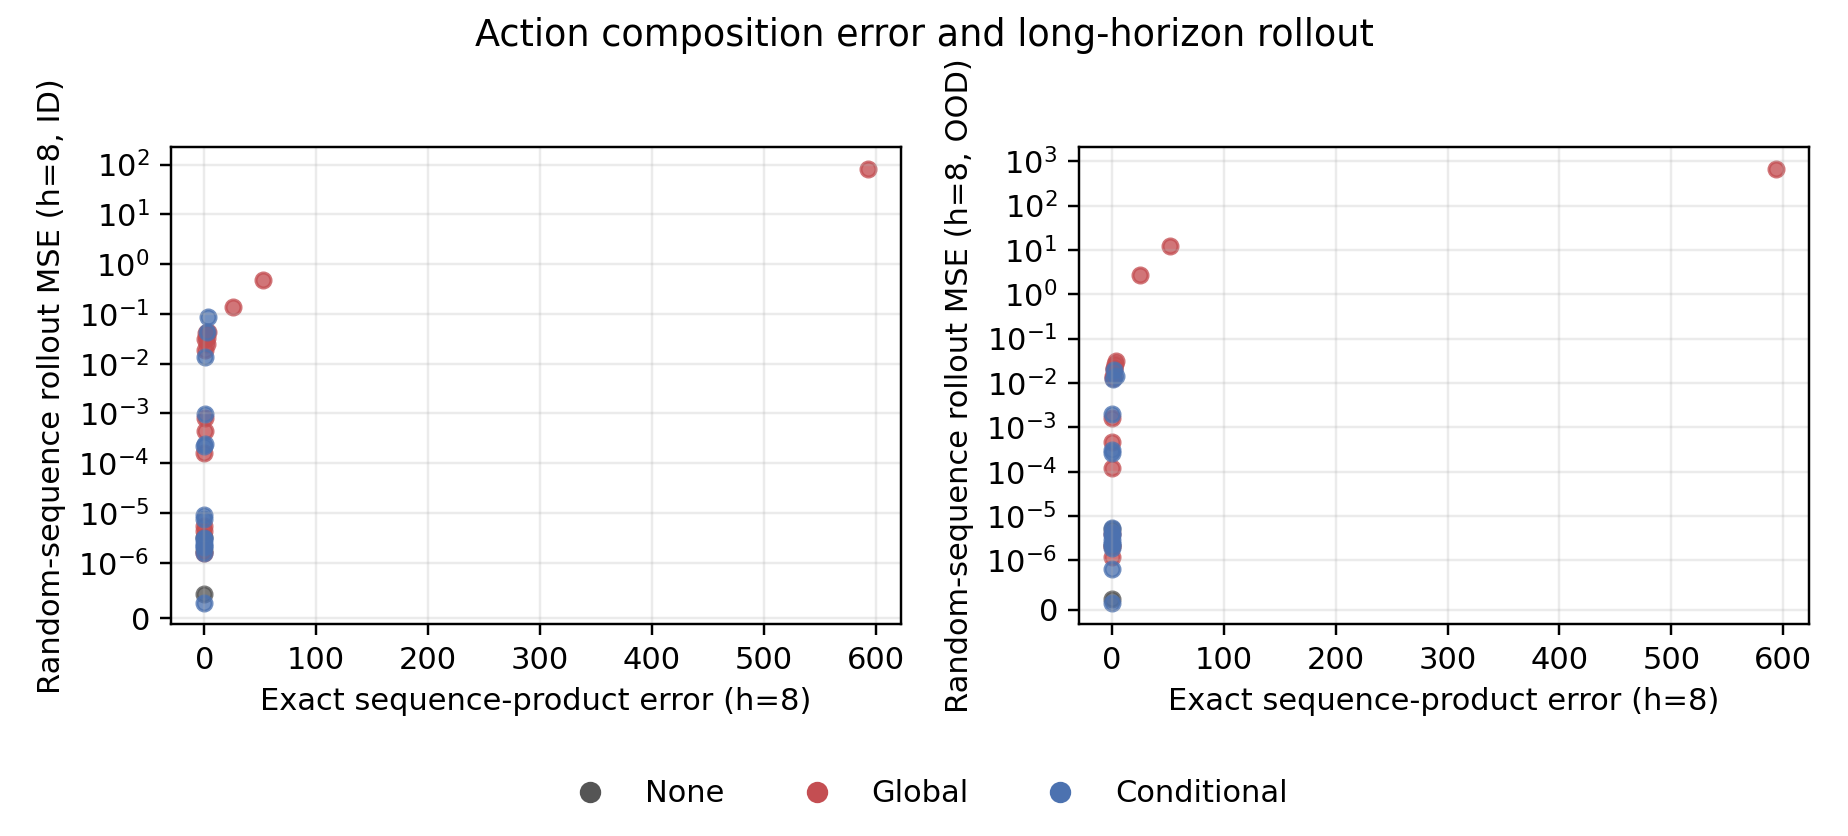
\includegraphics[width=\linewidth]{figures/composition_rollout_scatter.png}
\caption{Exact length-eight sequence-product error versus random-sequence
rollout error for the ID and OOD evaluation splits. Colors identify the none,
global, and conditional alignment interventions. The vertical axes use a
symmetric-log scale to retain both near-zero and high-error conditions. The
plot is a controlled synthetic association diagnostic, not evidence of causal
control or online-planning improvement.}
\label{fig:supp-action-composition}
\end{figure}
\endgroup

% Plan: State the surviving interpretation and its boundary before the next
% confound analysis.
The sequence audit strengthens the functional interpretation of the benchmark:
long-horizon error tracks the learned action-product structure more closely than
a one-step or pooled commutator summary alone. It does not establish that
alignment causes the association, that the relation transfers to nonlinear
LeWorldModel dynamics, or that it predicts task-level planning success.

\paragraph{Separating SIGReg-induced isotropy from alignment.}
The preceding intervention still leaves a possible confound: SIGReg may change
the latent covariance in a way that alters a covariance--predictor diagnostic
without changing the predictor geometry in a useful sense. We therefore cross
SIGReg weights $\{0,0.01,0.1\}$ with no alignment, global alignment, and
action-conditional alignment at weights $\{0.01,0.1,1\}$. Each of the 21
conditions is evaluated with three matched seeds, identical generated splits,
validation-MSE checkpoint selection, and the same learned pixel-world
benchmark. In addition to the two commutators, we record the latent stable rank
as an isotropy diagnostic and retain one-step, random-sequence $h=8$, and
ordered-composition readouts.

\begin{table}[H]
\centering
\scriptsize
\setlength{\tabcolsep}{2.2pt}
\caption{SIGReg $\times$ alignment phase diagnostic in the learned synthetic
pixel world. Entries are means over three seeds; per-seed values and sample
standard deviations are in the JSON artifact. The no-alignment row is the
matched baseline for each SIGReg weight. Stable rank is a covariance-shape
diagnostic, not a measure of representation quality.}
\label{tab:supp-sigreg-phase}
\resizebox{\linewidth}{!}{%
\begin{tabular}{lrrrrrrrr}
\toprule
SIGReg & Mode & Align. & One-step & $h=8$ & Composition & Global $\mathcal C$ & Conditional $\mathcal C$ & Stable rank \\
\midrule
0 & None & 0 & $1.219\times10^{-6}$ & $1.337\times10^{-6}$ & 0.0160 & 0.000593 & 0.000230 & 2.669 \\
0 & Global & 0.01 & $8.650\times10^{-5}$ & $8.583\times10^{-5}$ & 0.1221 & 0.0340 & 0.0195 & 3.138 \\
0 & Global & 0.1 & $1.107\times10^{-3}$ & $1.136\times10^{-3}$ & 0.3987 & 0.0431 & 0.0508 & 3.044 \\
0 & Global & 1 & $7.232\times10^{-3}$ & $7.567\times10^{-3}$ & 0.7255 & 0.0223 & 0.0751 & 2.213 \\
0 & Conditional & 0.01 & $6.792\times10^{-5}$ & $7.051\times10^{-5}$ & 0.1096 & 0.0853 & 0.0196 & 2.798 \\
0 & Conditional & 0.1 & $5.231\times10^{-4}$ & $5.501\times10^{-4}$ & 0.2973 & 0.0403 & 0.0208 & 3.787 \\
0 & Conditional & 1 & $6.729\times10^{-3}$ & $7.269\times10^{-3}$ & 0.8177 & 0.0347 & 0.0245 & 3.043 \\
\midrule
0.01 & None & 0 & $2.532\times10^{-4}$ & $2.616\times10^{-4}$ & 1.257 & 0.1834 & 0.2526 & 2.008 \\
0.01 & Global & 0.01 & $5.489\times10^{-4}$ & $5.550\times10^{-4}$ & 1.627 & 0.0642 & 0.1084 & 2.193 \\
0.01 & Global & 0.1 & $2.047\times10^{-3}$ & $2.004\times10^{-3}$ & 2.404 & 0.0384 & 0.0469 & 3.429 \\
0.01 & Global & 1 & $1.271\times10^{-2}$ & $1.352\times10^{-2}$ & 1.961 & 0.1003 & 0.0846 & 2.792 \\
0.01 & Conditional & 0.01 & $3.932\times10^{-4}$ & $4.205\times10^{-4}$ & 1.592 & 0.0191 & 0.0137 & 1.891 \\
0.01 & Conditional & 0.1 & $1.638\times10^{-3}$ & $1.729\times10^{-3}$ & 1.935 & 0.0270 & 0.0460 & 2.781 \\
0.01 & Conditional & 1 & $1.339\times10^{-2}$ & $1.432\times10^{-2}$ & 2.129 & 0.0302 & 0.0219 & 2.446 \\
\midrule
0.1 & None & 0 & $4.837\times10^{-4}$ & $5.068\times10^{-4}$ & 1.352 & 0.1031 & 0.0856 & 1.893 \\
0.1 & Global & 0.01 & $5.580\times10^{-4}$ & $5.779\times10^{-4}$ & 1.548 & 0.0263 & 0.0388 & 2.229 \\
0.1 & Global & 0.1 & $1.608\times10^{-3}$ & $1.665\times10^{-3}$ & 2.282 & 0.0185 & 0.0166 & 2.600 \\
0.1 & Global & 1 & $1.236\times10^{-2}$ & $1.236\times10^{-2}$ & 2.834 & 0.0513 & 0.0483 & 3.078 \\
0.1 & Conditional & 0.01 & $5.415\times10^{-4}$ & $5.683\times10^{-4}$ & 1.603 & 0.0214 & 0.0122 & 2.183 \\
0.1 & Conditional & 0.1 & $1.348\times10^{-3}$ & $1.387\times10^{-3}$ & 1.813 & 0.0197 & 0.0141 & 2.411 \\
0.1 & Conditional & 1 & $1.214\times10^{-2}$ & $1.268\times10^{-2}$ & 2.577 & 0.1021 & 0.0682 & 2.959 \\
\bottomrule
\end{tabular}
}
\end{table}

\begingroup
\renewcommand{\figurename}{Supplementary Figure}
\begin{figure}[H]
\centering
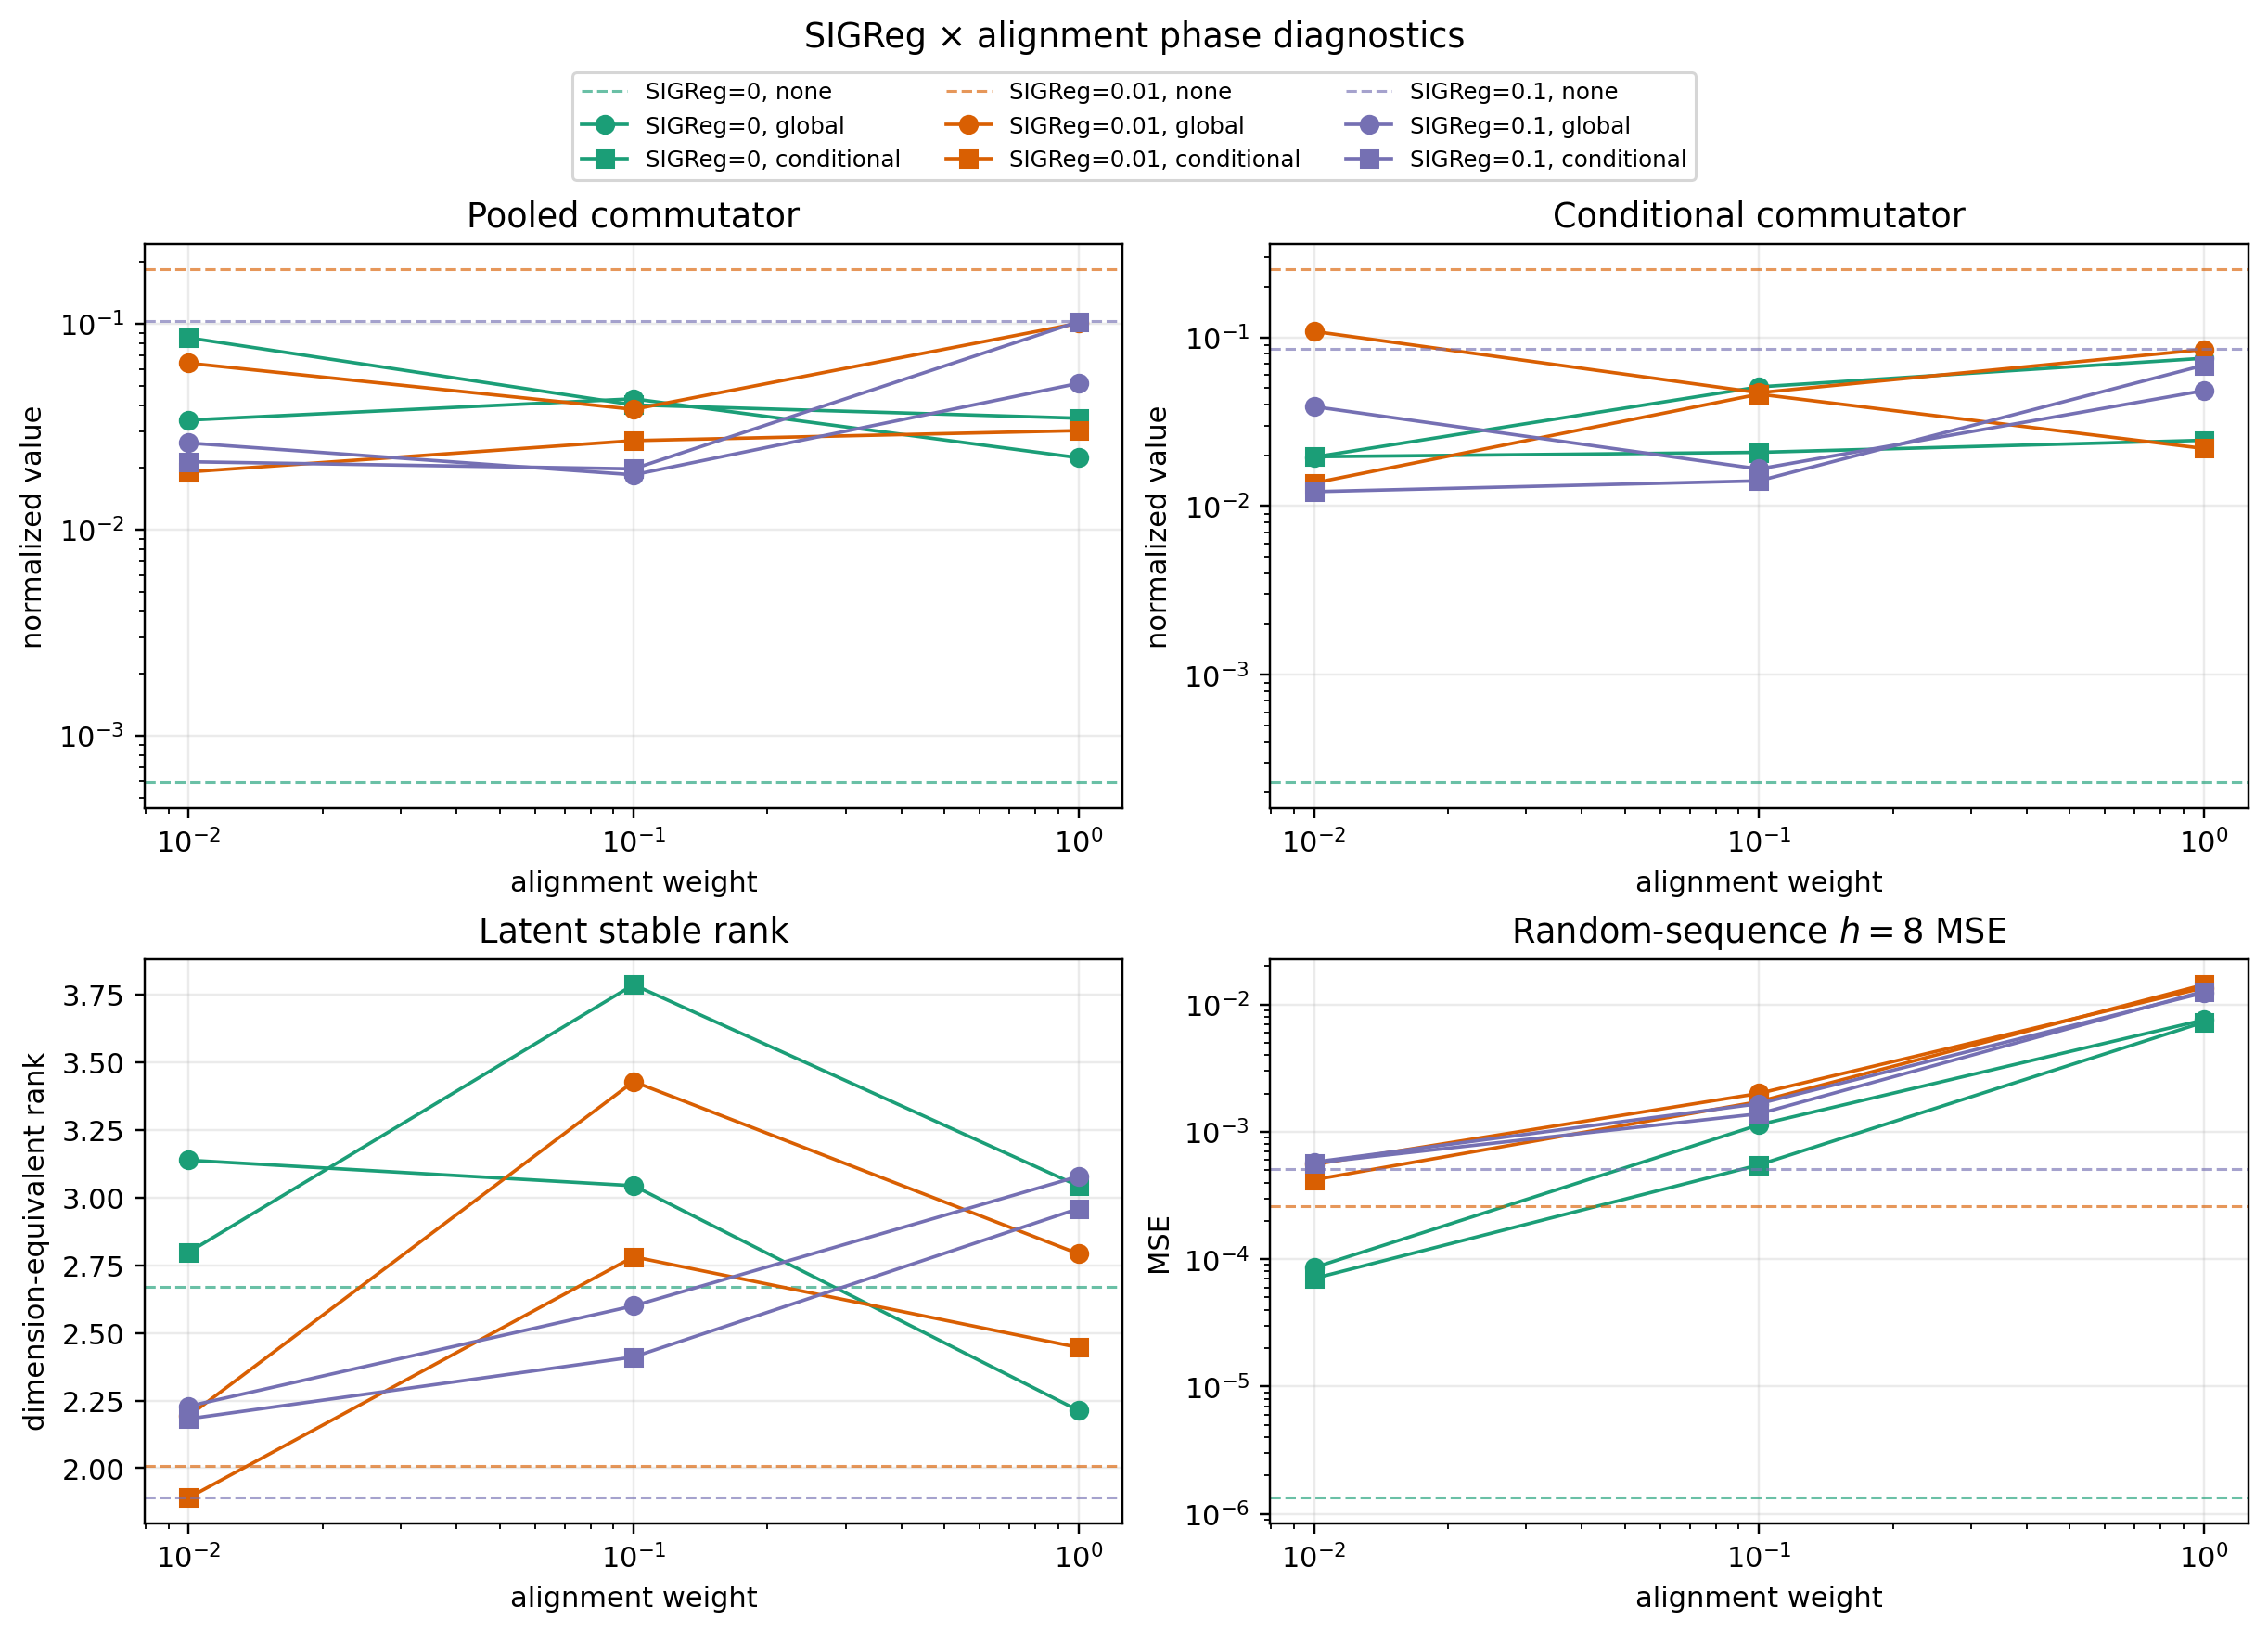
\includegraphics[width=\linewidth]{figures/sigreg_alignment_phase_diagnostics.png}
\caption{Phase diagnostics for the SIGReg--alignment cross-factorial sweep.
Dashed lines are the no-alignment baselines at each SIGReg weight; circles and
squares denote global and conditional alignment, respectively. Lower
commutators coexist with higher one-step, rollout, and composition errors in
many $\mathrm{SIGReg}>0$ conditions, so the diagnostic is not a sufficient
functional objective.}
\label{fig:supp-sigreg-phase}
\end{figure}
\endgroup

The phase table makes the confound explicit. At $\mathrm{SIGReg}=0$, adding
alignment generally raises both commutators and worsens the functional readouts.
At $\mathrm{SIGReg}=0.01$ and $0.1$, alignment often lowers the commutators
relative to the matched no-alignment baseline, while every aligned condition
has a higher mean $h=8$ error and composition error in this sweep. Stable rank
also moves with the regularizer and is non-monotone across alignment weights,
confirming that covariance shape and functional prediction are separate
estimands. This is CPU-only synthetic mechanism evidence: it rules out treating
commutator reduction as sufficient evidence of better prediction in this
setting, but it does not identify a universal causal effect or establish a
nonlinear LeWorldModel, PushT, online-control, or GPU result.

\subsection{Cross-source latent-dynamics transport in LeWorldModel}
\label{sec:supp-lewm-latent-transport}

The preceding frozen PushT analyses identify a dynamics-sensitive latent
subspace, but that identification alone does not show that the subspace is
transported by autoregressive prediction. We therefore performed a separate
cross-source audit. The covariance basis, raw dynamics cross-covariance basis,
and action-residualized dynamics basis were fitted on an internal frozen
latent export and transferred without refitting to the public external PushT
validation trajectories. The external evaluation used 21 episodes and 164
windows (up to eight windows per episode), with leave-one-episode-out fits and
episode-cluster bootstrap intervals.

For a basis $B$ and coordinate band $I$, let $z_t^{B,I}$ denote the selected
coordinates of the centered latent. We distinguish the encoded future
increment from the autoregressive increment by
\begin{equation}
\Delta_h^{B,I}=z_{t+h}^{B,I}-z_t^{B,I},\qquad
\widehat{\Delta}_h^{B,I}=\widehat z_{t+h}^{B,I}-z_t^{B,I},
\label{eq:supp-lewm-transport}
\end{equation}
where the second quantity uses the frozen predictor and the same observed
action sequence. A probe fitted on encoded trajectories was applied to both
quantities. The resulting predicted-$R^2$ contrast compares the transported
increment in the dynamics basis with a covariance or dimension-matched random
top-$8$ basis on the same held-out windows. This is deliberately a latent
transport estimand: it is not a physical-state decoder and does not intervene
on the environment.

\begin{table}[H]
\centering
\scriptsize
\setlength{\tabcolsep}{3pt}
\caption{Paired predicted-$R^2$ contrasts for the transferred dynamics top-$8$
basis. Each entry is dynamics basis minus the indicated control, with a 95\%
episode-cluster bootstrap interval. The basis is fit outside the external
validation trajectories.}
\label{tab:supp-lewm-transport}
\resizebox{\linewidth}{!}{%
\begin{tabular}{llrr}
\toprule
Action normalization & Horizon & Versus covariance & Versus random \\
\midrule
Public mean/std & $h=1$ & $+0.0678\ [0.0403,0.0973]$ & $+0.0622\ [0.0330,0.0989]$ \\
Public mean/std & $h=4$ & $+0.0908\ [0.0297,0.1626]$ & $+0.0460\ [0.0063,0.0927]$ \\
Public mean/std & $h=8$ & $+0.1788\ [0.0619,0.3462]$ & $+0.0670\ [0.0142,0.1240]$ \\
Validation z-score & $h=1$ & $+0.0546\ [-0.0130,0.1215]$ & $+0.0203\ [-0.0372,0.0808]$ \\
Validation z-score & $h=4$ & $+0.4272\ [0.1865,0.7096]$ & $+0.1384\ [0.0118,0.2933]$ \\
Validation z-score & $h=8$ & $+0.5373\ [0.3494,0.7201]$ & $+0.1470\ [0.0187,0.2797]$ \\
Raw action$/100$ & $h=1$ & $-0.0128\ [-0.0402,0.0106]$ & $+0.0133\ [-0.0232,0.0496]$ \\
Raw action$/100$ & $h=4$ & $+0.0628\ [-0.0675,0.2124]$ & $-0.0487\ [-0.1332,0.0225]$ \\
Raw action$/100$ & $h=8$ & $+0.0328\ [-0.1555,0.1820]$ & $-0.1485\ [-0.4477,0.0396]$ \\
\bottomrule
\end{tabular}}
\end{table}

Under the public normalization, the dynamics basis exceeds both controls at all
three horizons. Under validation-split z-scoring, the advantage is supported at
$h=4$ and $h=8$ but not at $h=1$. Under raw action scaling, all paired
intervals include zero. The transported dynamics top-$8$ predicted-$R^2$ in
the public arm is $0.9064$, $0.9057$, and $0.7134$ at $h=1,4,8$ respectively;
the decline at $h=8$ is evidence against a claim of perfect long-horizon
transport. The cross-normalization result therefore supports a conditional
latent-transport statement, not a normalization-invariant dynamics discovery.

The control hierarchy is important for interpretation. Action-only and
current-state-only probes are retained as predictive baselines, while the
rollout-increment probe tests whether the frozen autoregressive trajectory
preserves the transferred coordinates. The same external data also show that
action summaries explain most physical displacement in the available probe;
therefore the latent-transport result must not be relabeled as additional
physical-motion prediction, causal action effect, online planning, task
success, or retraining improvement. The complete machine-readable reports,
including the three normalization arms and source hashes, are included with
the experiment artifacts.

\subsection{Cross-horizon latent-displacement transport}
\label{sec:supp-cross-horizon-transport}

The preceding transfer test evaluates a fitted predictor readout at each
horizon. We add a complementary test that does not fit any readout on the
external trajectories. For each external window, let $z_{h}$ denote the
encoded future LeWM embedding at horizon $h$. For a source-fitted orthonormal
basis $B_{k}$, we measure the fraction of the encoded latent displacement
captured by its first $k$ coordinates:
\begin{equation}
\rho_{B_k}(h_a,h_b)=
\frac{\left\lVert (z_{h_b}-z_{h_a})^{\top}B_k\right\rVert_2^2}
{\left\lVert z_{h_b}-z_{h_a}\right\rVert_2^2+\epsilon},
\qquad (h_a,h_b)\in\{(1,2),(2,4),(4,8)\}.
\label{eq:supp-cross-horizon-share}
\end{equation}
Here $B_k$ is fitted only on the internal frozen latent export and is then
held fixed. We compare the dynamics cross-covariance basis with the covariance
basis and dimension-matched random subspaces; the conditional dynamics basis
is reported as an additional sensitivity control. The external sample has 21
episodes and 42 windows. Inference is clustered by episode, and the three
source fits are retained as separate estimates rather than pooled into a new
interval.

\begin{table}[H]
\centering
\scriptsize
\setlength{\tabcolsep}{3pt}
\caption{Cross-horizon transport of a source-fitted dynamics basis. Each row
reports the mean top-$8$ projection-energy share across three independent
source fits, followed by paired differences against the covariance and random
subspace controls. Positive differences favor the dynamics basis. The source
fit estimates are not pooled into a confidence interval; all three source
fits have the displayed sign.}
\label{tab:supp-cross-horizon-transport}
\begin{tabular}{lrrrcc}
\toprule
Encoded displacement & Dynamics share & $\Delta$ vs covariance & $\Delta$ vs random & Covariance sign & Random sign \\
\midrule
$z_{2}-z_{1}$ & 0.176089 & $+0.105223$ & $+0.134697$ & All positive & All positive \\
$z_{4}-z_{2}$ & 0.160430 & $+0.095658$ & $+0.119019$ & All positive & All positive \\
$z_{8}-z_{4}$ & 0.120726 & $+0.050672$ & $+0.079402$ & All positive & All positive \\
\bottomrule
\end{tabular}
\end{table}

The same conclusion holds for the wider top-$32$ band: the dynamics-minus-
covariance contrasts are $+0.179237$, $+0.173664$, and $+0.074898$ for the
three displacement spans, respectively, and every source fit remains
positive. This is stronger than the earlier source-domain readout because the
external trajectories are used only as held-out targets, not to define the
basis. It supports a conditional statement that the source-fitted dynamics
geometry captures external encoded latent evolution across multiple spans.
It does not establish that the coordinates represent extra physical motion:
the target in Eq.~\eqref{eq:supp-cross-horizon-share} is an embedding
displacement, while the separate action-conditioned physical probe does not
show incremental physical-motion predictability beyond observed actions.
Nor does this test establish normalization-invariant transport, causal
controllability, online planning, task success, or retraining improvement.

\subsection{Action-conditioned residual transport}
\label{sec:supp-action-residual-transport}

To make the action-related alternative explicit, we next remove the prediction
of a compact action-history probe before measuring the cross-horizon geometry.
For an external window from episode $e$, let $A^{e}_{a:b}$ contain the mean
action in each five-frame action block between horizons $a$ and $b$. The probe
$\widehat f_{-e}$ is fitted on all episodes except $e$, and the residual target
is
\begin{equation}
\widetilde{\Delta}^{e}_{a:b}=
\left(z^{e}_{b}-z^{e}_{a}\right)-
\widehat f_{-e}\!\left(A^{e}_{a:b}\right).
\label{eq:supp-action-residual}
\end{equation}
The feature vector concatenates the mean, first, and last action-block means;
this is the same compact action probe used by the physical-motion audit. We
use a ridge readout and evaluate it leave-one-episode-out. Thus, the action
residual for a held-out episode is not computed by a model trained on that
episode.

\begin{table}[H]
\centering
\scriptsize
\setlength{\tabcolsep}{3pt}
\caption{Action-conditioned residual transport under the public action
normalization. The action $R^2$ is cross-fitted against encoded latent
displacement; negative values indicate that this compact action summary does
not predict the target better than the training-centroid baseline. The final
two columns are top-$8$ dynamics-basis projection contrasts averaged over
three source fits.}
\label{tab:supp-action-residual-transport}
\begin{tabular}{lrrrr}
\toprule
Displacement & Action $R^2$ & Residual/raw energy & $\Delta$ vs covariance & $\Delta$ vs random \\
\midrule
$z_{2}-z_{1}$ & $-0.071033$ & 1.044834 & $+0.105807$ & $+0.117693$ \\
$z_{4}-z_{2}$ & $-0.176546$ & 1.144078 & $+0.090278$ & $+0.104822$ \\
$z_{8}-z_{4}$ & $-0.226125$ & 1.186186 & $+0.046750$ & $+0.073818$ \\
\bottomrule
\end{tabular}
\end{table}

The positive contrasts persist for every source fit and for all three action
normalization arms (public, validation-split z-score, and raw action divided by
100). However, the negative action-probe $R^2$ and residual/raw energy above
one are important diagnostics: the compact probe is weak for predicting this
latent target, so Eq.~\eqref{eq:supp-action-residual} must not be interpreted
as removing all action effects. The defensible conclusion is narrower: the
dynamics-basis enrichment is stable after the declared cross-fitted action
control in the encoded latent space. It still does not establish additional
physical-motion information, causal controllability, online planning, task
success, or retraining gains.

\subsection{Action-conditioned operator algebra}
\label{sec:supp-action-algebra}

The residual analysis above controls for an observed action summary but does
not test whether actions enter the latent transition in a compositional form.
We therefore fit an explicit low-dimensional action-conditioned map in each
leave-one-episode-out fold. Let $\xi_t$ be the rank-$16$ source-PCA coordinate
of either the encoded target trajectory or the autoregressively predicted
trajectory, and let $u_t$ be the mean of the normalized five-frame action block
aligned with the transition $\xi_t\to\xi_{t+1}$. The fitted map is
\begin{equation}
T_u(\xi)=A\xi+Bu+b,
\label{eq:supp-action-map}
\end{equation}
with a state-only map $T(\xi)=A_0\xi+b_0$ as the matched control. For the
primary audit, all maps are fitted on the other twenty episodes and scored
only on the held-out episode; the two windows per episode are never split
across folds. We additionally repeat the public-normalization audit with up
to eight windows per episode, retaining all available windows for short
episodes.

We evaluate action alignment by replacing $u_t$ with zero or with a cyclic
permutation from another held-out transition. We evaluate composition by
comparing repeated one-step application with a separately fitted direct map
$D_H(\xi_t,u_t,\ldots,u_{t+H-1})$:
\begin{equation}
\delta_H=\frac{\left\lVert
T_{u_{t+H-1}}\circ\cdots\circ T_{u_t}(\xi_t)
-D_H(\xi_t,u_t,\ldots,u_{t+H-1})\right\rVert_2}
{\left\lVert D_H(\xi_t,u_t,\ldots,u_{t+H-1})\right\rVert_2+\epsilon}.
\label{eq:supp-action-composition-defect}
\end{equation}
Finally, we report a negated-action return proxy,
\begin{equation}
\iota(\xi,u)=
\frac{\left\lVert T_{-u}(T_u(\xi))-\xi\right\rVert_2}
{\left\lVert\xi\right\rVert_2+\epsilon},
\label{eq:supp-action-inverse-proxy}
\end{equation}
which is an algebraic diagnostic rather than an assumption that contact
dynamics are physically reversible.

\begin{table}[H]
\centering
\scriptsize
\setlength{\tabcolsep}{3pt}
\caption{Cross-fitted action-alignment diagnostics on the external PushT
validation trajectories. Entries are means with 95\% episode-bootstrap
intervals. ``Action gain'' is state-only MSE minus action-conditioned MSE;
``permuted penalty'' is permuted-action MSE minus observed-action MSE.}
\label{tab:supp-action-algebra-alignment}
\resizebox{\linewidth}{!}{%
\begin{tabular}{lrrrrr}
\toprule
Trajectory source & State-only MSE & Action-conditioned MSE & Action gain & Zero penalty & Permuted penalty \\
\midrule
Encoded target & $0.6492$ & $0.6525$ & $-0.0033\ [-0.0137,0.0071]$ & $-0.0033\ [-0.0148,0.0077]$ & $+0.0158\ [0.0084,0.0248]$ \\
Autoregressive prediction & $0.6532$ & $0.6546$ & $-0.0014\ [-0.0117,0.0097]$ & $-0.0021\ [-0.0123,0.0085]$ & $+0.0147\ [0.0078,0.0222]$ \\
\bottomrule
\end{tabular}}
\end{table}

The action permutation penalty is positive for both trajectory sources, while
the independent one-step action gain and zero-action penalty are inconclusive.
Thus, the stronger supported statement is that the fitted latent transition is
sensitive to action--state alignment, not that a compact linear action term
provides an independent one-step predictor improvement.

\begin{table}[H]
\centering
\scriptsize
\setlength{\tabcolsep}{3pt}
\caption{Action composition and inverse-proxy diagnostics. Composition defect
is defined in Eq.~\eqref{eq:supp-action-composition-defect}; the final column
is the mean Eq.~\eqref{eq:supp-action-inverse-proxy}. The composed-minus-direct
MSE contrasts use the same held-out windows.}
\label{tab:supp-action-algebra-composition}
\resizebox{\linewidth}{!}{%
\begin{tabular}{llrrrr}
\toprule
Trajectory source & Horizon & Composition defect & Composed MSE & Direct MSE & Composed $-$ direct MSE \\
\midrule
Encoded target & 2 & $0.165$ & $1.679$ & $1.682$ & $-0.003\ [-0.021,0.017]$ \\
Encoded target & 4 & $0.583$ & $3.334$ & $3.349$ & $-0.016\ [-0.136,0.104]$ \\
Encoded target & 8 & $1.015$ & $5.163$ & $9.280$ & $-4.118\ [-5.709,-2.726]$ \\
Autoregressive prediction & 2 & $0.169$ & $1.655$ & $1.666$ & $-0.011\ [-0.028,0.006]$ \\
Autoregressive prediction & 4 & $0.565$ & $3.127$ & $3.246$ & $-0.119\ [-0.275,0.035]$ \\
Autoregressive prediction & 8 & $0.972$ & $4.042$ & $7.559$ & $-3.517\ [-4.829,-2.349]$ \\
\bottomrule
\end{tabular}}
\end{table}

Composition defect grows with horizon, but the composed-minus-direct contrast
is inconclusive at $H=2$ and $H=4$ and reverses at $H=8$ because the direct
high-dimensional map is itself poorly identified. The negated-action return
defect is $0.372$ for encoded targets and $0.350$ for predictions, and the
episode-level correlation between $H=8$ composition defect and observed
$H=8$ rollout MSE is weak (Pearson $-0.115$ and $0.228$, respectively).
Accordingly, these results support action-order sensitivity and expose a
non-compositionality diagnostic, but do not support a claim of physical inverse
consistency, causal controllability, or a monotone composition--rollout law.

To test whether this conclusion depends on using only two windows per episode,
we repeated the public-normalization audit with up to eight windows per
episode. The replication contains 164 windows from the same 21 episodes; the
two shortest episodes contribute six windows, and all other episodes contribute
eight. The folds, rank-$16$ PCA construction, ridge parameter, and episode
bootstrap are unchanged. The replication is summarized in
Tables~\ref{tab:supp-action-algebra-w8-alignment} and
\ref{tab:supp-action-algebra-w8-composition}.

\begin{table}[H]
\centering
\scriptsize
\setlength{\tabcolsep}{3pt}
\caption{Eight-window replication of action-alignment diagnostics under the
public action normalization. Entries are means with 95\% episode-bootstrap
intervals. The replication preserves the positive action-permutation penalty,
whereas the independent one-step action gain remains inconclusive.}
\label{tab:supp-action-algebra-w8-alignment}
\resizebox{\linewidth}{!}{%
\begin{tabular}{lrrr}
\toprule
Trajectory source & Action gain & Zero penalty & Permuted penalty \\
\midrule
Encoded target & $+0.0082\ [-0.0048,0.0214]$ & $+0.0078\ [-0.0057,0.0224]$ & $+0.0254\ [0.0144,0.0400]$ \\
Autoregressive prediction & $+0.0083\ [-0.0034,0.0202]$ & $+0.0077\ [-0.0048,0.0207]$ & $+0.0242\ [0.0148,0.0359]$ \\
\bottomrule
\end{tabular}}
\end{table}

\begin{table}[H]
\centering
\scriptsize
\setlength{\tabcolsep}{2pt}
\caption{Eight-window replication of composition diagnostics. Entries are
means with 95\% episode-bootstrap intervals. $\delta_H$ is the repeated
one-step versus direct-map defect; $\Delta_H$ is composed-minus-direct MSE.}
\label{tab:supp-action-algebra-w8-composition}
\resizebox{\linewidth}{!}{%
\begin{tabular}{lrrrrrr}
\toprule
Trajectory source & $\delta_2$ & $\delta_4$ & $\delta_8$ & $\Delta_2$ & $\Delta_4$ & $\Delta_8$ \\
\midrule
Encoded target & $0.285\ [0.239,0.337]$ & $0.608\ [0.526,0.708]$ & $0.883\ [0.834,0.929]$ & $+0.009\ [-0.005,0.023]$ & $+0.048\ [-0.026,0.121]$ & $-0.293\ [-0.567,-0.047]$ \\
Autoregressive prediction & $0.295\ [0.250,0.344]$ & $0.647\ [0.574,0.739]$ & $0.893\ [0.839,0.953]$ & $+0.006\ [-0.007,0.019]$ & $+0.061\ [-0.012,0.138]$ & $-0.189\ [-0.326,-0.051]$ \\
\bottomrule
\end{tabular}}
\end{table}

The replication therefore strengthens the protocol-level observation that
correct action--state pairing matters, but it does not promote the result to a
composition law. The defect increases from $H=2$ to $H=8$ in both trajectory
sources; $\Delta_H$ is compatible with zero at $H=2$ and $H=4$, then becomes
negative at $H=8$ because the separately fitted direct map is poorly
identified at that horizon. This non-monotone contrast is precisely why we do
not interpret the audit as evidence for an exact semigroup, a stable physical
inverse, or online planning.

As a scale-robustness check, we repeated the complete frozen audit with
validation-split z-scoring and with raw actions divided by $100$. The action
permutation penalty remains positive for encoded targets under all three
normalizations and for predicted trajectories under the public and
validation-split normalizations; the raw$/100$ predicted-trajectory interval
includes zero. The state-only versus action-conditioned gain changes sign or
becomes very small across arms, and the composition and inverse-proxy values
also move with the ridge scale. We therefore treat the public-normalization
table above as the primary arm inherited from the external temporal protocol
and the following values as a robustness audit, not as pooled evidence.

\begin{table}[H]
\centering
\scriptsize
\setlength{\tabcolsep}{3pt}
\caption{Normalization robustness for the external action-algebra audit. Entries
are means; the primary public-normalization arm reports bootstrap intervals in
Tables~\ref{tab:supp-action-algebra-alignment} and
\ref{tab:supp-action-algebra-composition}.}
\label{tab:supp-action-algebra-normalization}
\resizebox{\linewidth}{!}{%
\begin{tabular}{llrrr}
\toprule
Normalization & Trajectory source & Action gain & Permuted penalty & $H=8$ composition defect \\
\midrule
Public mean/std & Encoded target & $-0.0033$ & $+0.0158$ & $1.015$ \\
Public mean/std & Autoregressive prediction & $-0.0014$ & $+0.0147$ & $0.972$ \\
Validation z-score & Encoded target & $+0.0010$ & $+0.0244$ & $1.032$ \\
Validation z-score & Autoregressive prediction & $+0.0225$ & $+0.0422$ & $0.916$ \\
Raw action$/100$ & Encoded target & $+0.0038$ & $+0.0042$ & $0.877$ \\
Raw action$/100$ & Autoregressive prediction & $+0.0001$ & $+0.0001$ & $0.203$ \\
\bottomrule
\end{tabular}}
\end{table}

This sensitivity check rules out a normalization-invariant claim that the
compact linear action term always improves one-step prediction. It preserves a
more limited conclusion: action-order perturbations can be detected in the
latent operator, but their magnitude and the apparent long-horizon algebra
depend on action scaling and regularization.

\subsection{Conditional local transition geometry}
\label{sec:supp-conditional-operator-geometry}

The action-algebra audit establishes action-order sensitivity, but it does not
directly test whether different action regimes correspond to different local
transition maps. We therefore add a matched local-operator diagnostic on the
same frozen external validation protocol. For each leave-one-episode-out fold,
we fit a rank-$16$ PCA coordinate system on the remaining episodes and fit a
ridge row operator separately within two action bins. The primary condition
uses quantiles of the normalized five-frame action-block magnitude. A
direction condition uses quantiles of the cosine-like projection onto a
training-fold action axis; it tests whether the result is specific to direction
rather than only movement amplitude. The random partition preserves the two
bin sizes while independently permuting the labels in the training and held-out
folds. As a stronger control, the state-matched partition permutes labels only
within coarse strata of the first training-fold state-PCA coordinate. It
therefore preserves the condition-label composition within approximate state
regions while breaking action--transition alignment.

Let $A_1,\ldots,A_m$ denote the fitted row transition operators for the
action-aligned bins. We measure local transition-map heterogeneity by
\begin{equation}
\begin{aligned}
\mathcal{H}(A_{1:m})
&=\frac{2}{m(m-1)}\sum_{i<j}
\frac{\lVert A_i-A_j\rVert_F}
{\lVert A_i\rVert_F+\lVert A_j\rVert_F+\epsilon},\\
\Delta_{\mathcal H}^{\mathrm{rand}}
&=\mathcal{H}_{\mathrm{aligned}}-\mathcal{H}_{\mathrm{random}},\\
\Delta_{\mathcal H}^{\mathrm{state}}
&=\mathcal{H}_{\mathrm{aligned}}-\mathcal{H}_{\mathrm{state\text{-}matched}}.
\end{aligned}
\label{eq:supp-local-operator-heterogeneity}
\end{equation}
The estimand in Eq.~\eqref{eq:supp-local-operator-heterogeneity} is a
descriptive difference between fold-fitted linear maps. It is not a nonlinear
Jacobian estimate and does not assume that the action partition is a causal
intervention.

\begin{table}[H]
\centering
\scriptsize
\setlength{\tabcolsep}{3pt}
\caption{Conditional local transition geometry on the public PushT validation
set. Each row reports mean differences between the action-aligned partition and
the global random or state-matched null, with 95\% episode-bootstrap intervals.
$\Delta\mathcal H$ is the local operator heterogeneity from
Eq.~\eqref{eq:supp-local-operator-heterogeneity}; $\Delta R^2$ is the
state-matched held-out transition-prediction contrast. All operators are fit
outside the held-out episode.}
\label{tab:supp-conditional-operator-geometry}
\resizebox{\linewidth}{!}{%
\begin{tabular}{llrrr}
\toprule
Normalization & Trajectory source / condition & $\Delta\mathcal H$ vs random & $\Delta\mathcal H$ vs state & $\Delta R^2$ vs state \\
\midrule
Public mean/std & Encoded / magnitude & $+0.0515\ [0.0478,0.0552]$ & $+0.0518\ [0.0487,0.0550]$ & $-0.0046\ [-0.0297,0.0170]$ \\
Public mean/std & Encoded / direction & $+0.0456\ [0.0416,0.0499]$ & $+0.0467\ [0.0430,0.0505]$ & $-0.0431\ [-0.1228,0.0283]$ \\
Public mean/std & Predicted / magnitude & $+0.0613\ [0.0575,0.0649]$ & $+0.0609\ [0.0564,0.0658]$ & $+0.0101\ [-0.0416,0.0487]$ \\
Public mean/std & Predicted / direction & $+0.0558\ [0.0517,0.0599]$ & $+0.0509\ [0.0468,0.0546]$ & $-0.0365\ [-0.0984,0.0133]$ \\
Validation z-score & Encoded / magnitude & $+0.0517\ [0.0488,0.0546]$ & $+0.0504\ [0.0465,0.0547]$ & $+0.0273\ [-0.0002,0.0596]$ \\
Validation z-score & Encoded / direction & $+0.0418\ [0.0381,0.0455]$ & $+0.0416\ [0.0386,0.0447]$ & $-0.0706\ [-0.1460,-0.0034]$ \\
Validation z-score & Predicted / magnitude & $+0.0375\ [0.0345,0.0406]$ & $+0.0405\ [0.0367,0.0444]$ & $-0.0072\ [-0.0324,0.0167]$ \\
Validation z-score & Predicted / direction & $+0.0440\ [0.0398,0.0484]$ & $+0.0437\ [0.0403,0.0468]$ & $-0.0487\ [-0.1218,0.0080]$ \\
Raw action$/100$ & Encoded / magnitude & $+0.0409\ [0.0373,0.0445]$ & $+0.0412\ [0.0375,0.0451]$ & $-0.0099\ [-0.0257,0.0057]$ \\
Raw action$/100$ & Encoded / direction & $+0.0437\ [0.0399,0.0484]$ & $+0.0439\ [0.0398,0.0482]$ & $-0.0502\ [-0.1157,-0.0042]$ \\
Raw action$/100$ & Predicted / magnitude & $+0.0093\ [0.0083,0.0103]$ & $+0.0094\ [0.0086,0.0102]$ & $+0.0013\ [-0.0410,0.0406]$ \\
Raw action$/100$ & Predicted / direction & $+0.0111\ [0.0101,0.0121]$ & $+0.0117\ [0.0108,0.0127]$ & $-0.0097\ [-0.0254,0.0008]$ \\
\bottomrule
\end{tabular}}
\end{table}

The local heterogeneity contrast against the state-matched null is positive
with a positive bootstrap lower bound in all twelve source--condition--
normalization cells. This is the strongest conclusion licensed by the
diagnostic: action-aligned partitions reveal latent transition-map
heterogeneity beyond both a bin-size null and a coarse state-only null, and the
effect survives the direction control and all three action normalizations. The
magnitude varies substantially, especially for the predicted trajectory under
raw action scaling. The held-out $R^2$ contrast is not uniformly positive;
direction conditioning is negative in all three normalization arms. For an
additional granularity sensitivity check, we repeat the public-normalization
state-matched permutation with 4, 8, and 16 first-coordinate strata. The
resulting local-heterogeneity contrasts are shown in
Table~\ref{tab:supp-conditional-operator-strata}; every source--condition
combination retains a positive lower confidence bound at all three
stratification resolutions, with 16 test rows covered per held-out fold. Thus,
detectable action-dependent regime structure must not be reported as a
prediction gain, a causal action effect, an online-planning improvement, or
evidence that an alignment regularizer would improve the trained model.

\begin{table}[H]
\centering
\scriptsize
\setlength{\tabcolsep}{3pt}
\caption{Sensitivity of the state-matched null to coarse state-stratum count
on the public PushT validation set. Each cell reports the mean
$\Delta\mathcal H^{\mathrm{state}}$ and its 95\% episode-bootstrap interval
for 4, 8, or 16 first-coordinate strata. All reports use the same 21 held-out
episodes and 42 windows, with 2,000 episode-cluster bootstrap replicates per
cell. The check concerns the granularity of a descriptive null, not a claim
that any stratum count identifies a physical state partition.}
\label{tab:supp-conditional-operator-strata}
\resizebox{\linewidth}{!}{%
\begin{tabular}{llccc}
\toprule
Trajectory source & Condition & 4 strata & 8 strata & 16 strata \\
\midrule
Encoded & Magnitude & $+0.05107\ [0.04723,0.05477]$ & $+0.05178\ [0.04868,0.05496]$ & $+0.05247\ [0.04861,0.05622]$ \\
Encoded & Direction & $+0.04353\ [0.03975,0.04762]$ & $+0.04674\ [0.04297,0.05049]$ & $+0.04673\ [0.04327,0.05017]$ \\
Predicted & Magnitude & $+0.06232\ [0.05970,0.06491]$ & $+0.06091\ [0.05639,0.06584]$ & $+0.05930\ [0.05483,0.06420]$ \\
Predicted & Direction & $+0.05431\ [0.05081,0.05798]$ & $+0.05091\ [0.04681,0.05462]$ & $+0.05208\ [0.04776,0.05587]$ \\
\bottomrule
\end{tabular}}
\end{table}

\subsection{Leakage-controlled forward readout of latent dynamics}
\label{sec:supp-forward-dynamics-readout}

The projection-share and rollout-intervention measurements above show that a
source-fitted dynamics basis is structurally and functionally involved in a
frozen latent rollout. A stricter test asks whether the same information can
be read out \emph{forward}: the future target must not be supplied as an
input. We therefore use the released public PushT validation episodes and
fit ridge probes in a leave-one-episode-out protocol. For each window, the
features are the current latent coordinates in a source-fitted basis band,
future action summaries, or their concatenation. The target is the future
increment projected into the fixed top-eight coordinates of the
source-fitted dynamics basis. Past-action and globally deranged-action
features are temporal controls. All source bases are fit on a separate
frozen latent export; no basis is refit on the external episodes.

\begin{table}[H]
\centering
\scriptsize
\setlength{\tabcolsep}{3pt}
\caption{Leakage-controlled forward readout of a fixed dynamics target at
$h=8$. Each row uses the same target, 21 held-out episodes, eight windows per
episode when available, and 2,000 episode-bootstrap replicates. $R^2$ is
computed on the held-out episode using the training-fold target mean; the
gain is the paired state-plus-action minus action-only contrast. The final
column compares each input basis with the dynamics top-8 input on the same
target.}
\label{tab:supp-forward-dynamics-readout}
\resizebox{\linewidth}{!}{%
\begin{tabular}{lrrr r}
\toprule
Input basis (top-8) & Action $R^2$ & State+action $R^2$ & Gain over action & Dynamics minus input \\
\midrule
Covariance & $+0.016\ [-0.044,+0.083]$ & $-0.077\ [-0.182,+0.011]$ & $-0.093\ [-0.183,-0.010]$ & $+0.562\ [0.474,0.678]$ \\
Dynamics & $+0.016\ [-0.044,+0.083]$ & $+0.485\ [0.423,+0.544]$ & $+0.469\ [0.401,+0.536]$ & -- \\
Residual & $+0.016\ [-0.044,+0.083]$ & $-0.040\ [-0.119,+0.034]$ & $-0.056\ [-0.116,+0.004]$ & $+0.525\ [0.456,0.607]$ \\
Random & $+0.016\ [-0.044,+0.083]$ & $-0.087\ [-0.168,-0.012]$ & $-0.103\ [-0.151,-0.058]$ & $+0.572\ [0.508,0.643]$ \\
\bottomrule
\end{tabular}}
\end{table}

The specificity is not an artifact of one action preprocessing or one ridge
choice. With the matched-band target, the dynamics top-8 state-plus-action
gain is $+0.469\ [0.401,0.536]$, $+0.468\ [0.400,0.534]$, and
$+0.477\ [0.403,0.550]$ under public mean/std, validation-split $z$-score,
and raw-action$/100$ preprocessing, respectively. For ridge values
$10^{-3},10^{-2},10^{-1}$, the fixed-target dynamics joint $R^2$ is
$0.479$, $0.485$, and $0.498$, while its gain over action is
$+0.467$, $+0.469$, and $+0.466$. Past-action gains remain negative at
$h=8$ (approximately $-0.059$ for the dynamics input), and deranged-action
controls do not reproduce the positive forward readout.

The target-resolution control is essential. Predicting the complete
192-dimensional latent increment gives a dynamics-top-8 state-plus-action
gain of $-0.038\ [-0.059,-0.020]$ at $h=8$. Accordingly, the evidence
supports a source-defined, band-level forward-predictive diagnostic rather
than a claim that the extracted subspace predicts the entire latent
transition. The target remains an encoded latent quantity, and the protocol
contains no physical intervention, causal action manipulation, online planner,
or task-success endpoint; none of these stronger claims is made.
As an explicit physical-target negative control, the separate normalized
physical-displacement probe gives an incremental $R^2$ of
$-0.120\ [-0.174,-0.074]$ over the compact action summary for the dynamics
top-8 predicted increment at $h=8$. Thus the positive readout should be
interpreted as encoded-latent predictive information, not as additional
physical-motion prediction.

To expose the temporal structure rather than report only the selected $h=8$
cell, we summarize the complete horizon profile in
Table~\ref{tab:supp-forward-dynamics-profile}. At the fixed dynamics target,
the dynamics top-8 gain is small and uncertain at $h=1$ but becomes positive
at $h=4$ and $h=8$. The joint future-versus-past contrast is also positive at
$h=8$, while the corresponding future-versus-deranged contrast is weaker;
these are temporal-predictive controls, not causal tests. The matched-band
analysis shows that the middle dynamics band is also predictive at the longer
horizons. This is useful negative information: the result identifies a
distributed source-defined dynamics geometry, not a claim that a single top
covariance band contains all relevant motion information.

\begin{table}[H]
\centering
\scriptsize
\setlength{\tabcolsep}{3pt}
\caption{Multi-horizon profile of the leakage-controlled forward readout.
Entries are mean $R^2$ or paired $R^2$ contrasts with 95\% held-out-episode
bootstrap intervals. The fixed target is the source-defined dynamics top-8
increment; the matched-band row uses the middle dynamics band as both input
and target. The future/past column compares joint state-plus-action features.}
\label{tab:supp-forward-dynamics-profile}
\resizebox{\linewidth}{!}{%
\begin{tabular}{llrrrrr}
\toprule
Input & $h$ & Action & State only & State+action & Gain over action & Future--past (joint) \\
\midrule
Dynamics top-8 & 1 & $+0.045\ [0.015,0.076]$ & $+0.085\ [0.011,0.147]$ & $+0.102\ [0.037,0.155]$ & $+0.056\ [-0.013,0.120]$ & $-0.015\ [-0.045,0.015]$ \\
Dynamics top-8 & 4 & $+0.026\ [-0.037,0.090]$ & $+0.493\ [0.447,0.535]$ & $+0.489\ [0.435,0.542]$ & $+0.462\ [0.398,0.536]$ & $+0.014\ [-0.011,0.036]$ \\
Dynamics top-8 & 8 & $+0.016\ [-0.044,0.085]$ & $+0.489\ [0.438,0.539]$ & $+0.485\ [0.425,0.543]$ & $+0.469\ [0.402,0.532]$ & $+0.029\ [0.002,0.062]$ \\
Covariance top-8 & 8 & $+0.016\ [-0.044,0.085]$ & $-0.072\ [-0.158,0.003]$ & $-0.077\ [-0.180,0.009]$ & $-0.093\ [-0.180,-0.013]$ & $+0.040\ [-0.009,0.087]$ \\
Residual top-8 & 8 & $+0.016\ [-0.044,0.085]$ & $-0.036\ [-0.096,0.026]$ & $-0.040\ [-0.114,0.036]$ & $-0.056\ [-0.120,0.002]$ & $+0.051\ [-0.003,0.107]$ \\
Matched dynamics middle & 8 & $-0.008\ [-0.046,0.027]$ & $+0.441\ [0.395,0.490]$ & $+0.423\ [0.376,0.473]$ & $+0.431\ [0.380,0.480]$ & -- \\
\bottomrule
\end{tabular}}
\end{table}

\subsection{Rank- and target-specificity of latent dynamics}
\label{sec:supp-rank-target-specificity}

The preceding forward readout establishes predictive information for a fixed
source-defined dynamics target. We next test whether that information is
specific to the corresponding latent geometry rather than a generic benefit
of adding coordinates. Let $B$ be a source-fitted orthonormal basis and let
$B_{k}$ denote its first $k$ columns. For each external window we form
\begin{equation}
\Delta^{(B,k)}_{h} = (z_{t+h}-z_t)^\top B_k,
\qquad
\Delta^{\mathrm{phys}}_{h}
 = \operatorname{wrap}(s_{t+h}-s_t),
\label{eq:supp-rank-target}
\end{equation}
where $z$ is the encoded latent and $s$ is the five-dimensional physical
state. We use $k\in\{1,2,4,8,16,32\}$ and $h\in\{1,4,8\}$. The four
target families are the dynamics-basis top-8 increment, residual-basis top-8
increment, full 192-dimensional increment, and physical displacement. The
predictors are the current coordinates in each transferred basis, observed
future-action summaries, or their concatenation. Bases are fitted on the
separate internal frozen export and never refit on the external windows.

Every fit leaves one complete episode out. The reported incremental $R^2$ is
the paired, window-level difference between the joint and action-only
readouts; its interval is an episode-cluster bootstrap over the same held-out
windows. This paired construction preserves the action baseline and avoids
subtracting two unrelated confidence intervals.

\begin{table}[H]
\centering
\scriptsize
\setlength{\tabcolsep}{3pt}
\caption{Target-specificity controls for the transferred top-8 subspaces. Entries are paired incremental $R^2$ over the observed-action baseline with 95\% episode-cluster bootstrap intervals. The target is fixed within each row; positive values mean that the indicated current latent coordinates add predictive information beyond the action summary.}
\label{tab:supp-rank-target-controls}
\resizebox{\linewidth}{!}{%
\begin{tabular}{llrr}
\toprule
Target & Input basis & $h=4$ & $h=8$ \\
\midrule
Dynamics-band latent increment & Dynamics top-8 & $+0.349\ [0.233,0.461]$ & $+0.255\ [0.058,0.461]$ \\
Dynamics-band latent increment & Covariance top-8 & $-0.453\ [-0.909,-0.188]$ & $-0.761\ [-1.585,-0.194]$ \\
Dynamics-band latent increment & Random top-8 & $-0.278\ [-0.509,-0.068]$ & $-0.361\ [-0.579,-0.159]$ \\
Residual-band latent increment & Residual top-8 & -- & $+0.279\ [0.124,0.447]$ \\
Residual-band latent increment & Dynamics top-8 & -- & $-0.255\ [-0.445,-0.100]$ \\
Physical displacement & Dynamics top-8 & $-0.098\ [-0.204,-0.027]$ & $-0.209\ [-0.492,-0.022]$ \\
Full latent increment & Dynamics top-8 & $-0.238\ [-0.398,-0.101]$ & $-0.294\ [-0.493,-0.129]$ \\
\bottomrule
\end{tabular}}
\end{table}

The complete rank curve for the dynamics-band target is shown below. At
$h=4$, the dynamics basis becomes positive from $k=2$ through $k=8$, while
the covariance, residual, and random controls remain negative. At $h=8$,
the same basis is positive at $k=2,4,8$ but degrades when the rank is
expanded, which is why the top-8 result is treated as a compact
source-defined diagnostic rather than an optimal universal rank.

\begin{table}[H]
\centering
\scriptsize
\setlength{\tabcolsep}{3pt}
\caption{Complete rank curve for the dynamics-band latent target. Cells are mean paired incremental $R^2$ over the observed-action baseline; the ranks were fixed before evaluating the target-specific contrasts.}
\label{tab:supp-rank-curve}
\resizebox{\linewidth}{!}{%
\begin{tabular}{lrrrrrr|rrrrrr}
\toprule
 & \multicolumn{6}{c|}{$h=4$} & \multicolumn{6}{c}{$h=8$} \\
Input basis & $k=1$ & $2$ & $4$ & $8$ & $16$ & $32$ & $k=1$ & $2$ & $4$ & $8$ & $16$ & $32$ \\
\midrule
Dynamics & $-0.050$ & $-0.150$ & $-0.212$ & $+0.349$ & $-1.058$ & $-3.399$ & $-0.002$ & $+0.018$ & $+0.020$ & $+0.255$ & $-0.237$ & $-1.679$ \\
Covariance & $-0.024$ & $-0.117$ & $-0.186$ & $-0.453$ & $-1.729$ & $-8.109$ & $-0.058$ & $-0.075$ & $-0.129$ & $-0.761$ & $-1.152$ & $-4.288$ \\
Residual & $-0.045$ & $-0.086$ & $-0.160$ & $-0.370$ & $-1.036$ & $-3.836$ & $-0.013$ & $-0.034$ & $-0.058$ & $-0.350$ & $-1.263$ & $-4.152$ \\
Random & $-0.052$ & $-0.067$ & $-0.106$ & $-0.278$ & $-1.152$ & $-6.403$ & $-0.029$ & $-0.045$ & $-0.151$ & $-0.361$ & $-0.711$ & $-3.174$ \\
\bottomrule
\end{tabular}}
\end{table}

The pattern is therefore target-specific rather than a generic coordinate
augmentation effect: dynamics coordinates help the dynamics-band target,
residual coordinates help the residual-band target, and neither result
transfers into additional physical-displacement prediction beyond observed
actions. The full-latent negative control further limits the claim to
source-defined latent bands. These are frozen predictive diagnostics; they do
not establish a physical causal mechanism, controllability, online planning,
or task success.

\subsection{Cross-horizon transfer of the readout}
\label{sec:supp-cross-horizon-readout}

The preceding rank curves fit a separate readout at each horizon. We add a
strict temporal-transfer control to test whether the source-defined
subspaces retain a predictive role when the readout is estimated at one
horizon and evaluated at another. For a source horizon $h_s$ and target
horizon $h_t$, let $\widehat f^{(h_s)}_{-e}$ denote a ridge readout fitted on
all episodes except $e$ using the action summary and current latent
coordinates, with the target formed at $h_s$. We evaluate the same fitted
coefficients on the held-out episode at $h_t$ and report
\begin{equation}
\Gamma_{B}^{h_s\!\to h_t}
 = R^2\!\left(\widehat f^{(h_s)}_{B,-e};Y^{(h_t)}_e\right)
 - R^2\!\left(\widehat f^{(h_s)}_{A,-e};Y^{(h_t)}_e\right),
\label{eq:supp-cross-horizon-readout}
\end{equation}
where $B$ is the current-latent basis and $A$ is the observed-action
summary. The episode is held out from both fits, and the source-fitted
dynamics, residual, covariance, and random bases are never refit. We
predeclare the forward transfer cells $1\!\to4$, $1\!\to8$, and $4\!\to8$;
the reverse cells are retained in the machine-readable artifact because
cross-horizon $R^2$ is not symmetric when the target scale changes.

\begin{table}[H]
\centering
\scriptsize
\setlength{\tabcolsep}{3pt}
\caption{Cross-horizon readout transfer at rank eight. Each cell is
incremental $R^2$ over the observed-action summary, with a 95\% episode-cluster
bootstrap interval. A readout is fitted at the source horizon and evaluated at
the target horizon on a held-out episode.}
\label{tab:supp-cross-horizon-readout}
\resizebox{\linewidth}{!}{%
\begin{tabular}{llrrrr}
\toprule
Train $\to$ test & Target & Dynamics & Covariance & Residual & Random \\
\midrule
$1\to4$ & Dynamics band & $+0.083\ [0.027,0.136]$ & $-0.207\ [-0.456,-0.056]$ & $-0.056\ [-0.125,0.001]$ & $-0.097\ [-0.217,0.008]$ \\
$1\to8$ & Dynamics band & $+0.037\ [-0.003,0.072]$ & $-0.132\ [-0.291,-0.010]$ & $-0.086\ [-0.165,-0.027]$ & $-0.046\ [-0.105,0.009]$ \\
$4\to8$ & Dynamics band & $+0.364\ [0.156,0.602]$ & $-0.430\ [-0.765,-0.182]$ & $-0.601\ [-1.455,-0.103]$ & $-0.188\ [-0.348,-0.039]$ \\
$1\to4$ & Residual band & $-0.030\ [-0.089,0.035]$ & $-0.065\ [-0.132,-0.014]$ & $+0.041\ [0.011,0.072]$ & $-0.021\ [-0.065,0.021]$ \\
$1\to8$ & Residual band & $-0.011\ [-0.036,0.014]$ & $-0.009\ [-0.028,0.009]$ & $+0.053\ [0.029,0.076]$ & $-0.008\ [-0.042,0.026]$ \\
$4\to8$ & Residual band & $-0.112\ [-0.206,-0.025]$ & $-0.020\ [-0.090,0.046]$ & $+0.177\ [0.108,0.252]$ & $-0.129\ [-0.261,-0.022]$ \\
\bottomrule
\end{tabular}}
\end{table}

The main forward-transfer result is the $4\to8$ cell. For the dynamics-band
target, the dynamics top-8 input exceeds the random and covariance controls by
paired contrasts of $+0.553$ $[+0.351,+0.773]$ and $+0.794$
$[+0.441,+1.216]$, respectively. For the residual-band target, the residual
top-8 input exceeds the dynamics input by $+0.290$
$[+0.150,+0.421]$. The same double dissociation is visible in the $1\to4$
and $1\to8$ cells, although the effects are smaller. The paired contrasts,
including all nine source--target horizon combinations and the reverse
direction, are included in the accompanying JSON and Markdown artifact.
This cross-horizon result strengthens the interpretation as a source-defined
latent predictive subspace, but it remains a frozen association beyond an
observed action summary. It does not establish a physical state variable,
causal action effect, online planning, task success, or retraining gain.

\subsubsection{Normalization and window-density robustness}
\label{sec:supp-cross-horizon-robustness}

The cross-horizon result is not tied to the public action normalization or to
the two-window sampling density. We repeat the complete frozen readout for
public normalization, validation-split z-scoring, and raw actions divided by
$100$, using two, four, and up to eight windows per episode. All nine cells
retain the same 21 held-out episodes, leave-one-episode-out fitting, rank-$8$
source bases, and 2,000 episode-cluster bootstrap replicates. Short episodes
contribute fewer than eight windows when the requested density is infeasible;
the resulting totals are therefore 42, 84, and 164 windows.

Table~\ref{tab:supp-cross-horizon-robustness} reports the predeclared forward
contrasts. The dynamics-minus-random contrast is positive in every cell for
$1\to4$, $1\to8$, and $4\to8$, and every corresponding 95\% episode-bootstrap
lower bound is above zero. The $4\to8$ residual-minus-dynamics contrast is
also positive in every cell. Thus the source-defined dynamics and residual
coordinates retain target-specific predictive roles across the tested
normalizations and sampling densities. This is evidence for robust
cross-horizon transfer of a frozen latent readout, not a claim of
normalization-invariant dynamics discovery or causal action influence.

\begin{table}[H]
\centering
\scriptsize
\setlength{\tabcolsep}{3pt}
\caption{Normalization and window-density robustness of the rank-$8$
cross-horizon readout. Entries are paired mean contrasts with 95\%
episode-cluster bootstrap intervals. ``D--R'' is dynamics minus random for the
dynamics-band target; ``R--D'' is residual minus dynamics for the residual-band
target.}
\label{tab:supp-cross-horizon-robustness}
\resizebox{\linewidth}{!}{%
\begin{tabular}{llrrrrr}
\toprule
Normalization & Windows/episode & Episodes $\times$ windows & D--R $1\to4$ & D--R $1\to8$ & D--R $4\to8$ & R--D $4\to8$ \\
\midrule
Public & 2 & $21\times42$ & $+0.180\,[+0.097,+0.273]$ & $+0.082\,[+0.031,+0.140]$ & $+0.553\,[+0.351,+0.773]$ & $+0.290\,[+0.150,+0.421]$ \\
Public & 4 & $21\times84$ & $+0.154\,[+0.120,+0.193]$ & $+0.090\,[+0.064,+0.117]$ & $+0.433\,[+0.268,+0.593]$ & $+0.317\,[+0.209,+0.431]$ \\
Public & 8 & $21\times164$ & $+0.160\,[+0.131,+0.188]$ & $+0.120\,[+0.096,+0.144]$ & $+0.458\,[+0.357,+0.556]$ & $+0.219\,[+0.150,+0.290]$ \\
Val.-split $z$ & 2 & $21\times42$ & $+0.178\,[+0.097,+0.269]$ & $+0.081\,[+0.030,+0.138]$ & $+0.556\,[+0.349,+0.780]$ & $+0.288\,[+0.151,+0.419]$ \\
Val.-split $z$ & 4 & $21\times84$ & $+0.153\,[+0.120,+0.192]$ & $+0.089\,[+0.063,+0.116]$ & $+0.434\,[+0.268,+0.595]$ & $+0.317\,[+0.208,+0.433]$ \\
Val.-split $z$ & 8 & $21\times164$ & $+0.160\,[+0.131,+0.187]$ & $+0.119\,[+0.095,+0.143]$ & $+0.459\,[+0.358,+0.557]$ & $+0.218\,[+0.148,+0.288]$ \\
Raw$/100$ & 2 & $21\times42$ & $+0.185\,[+0.101,+0.280]$ & $+0.087\,[+0.036,+0.147]$ & $+0.484\,[+0.319,+0.662]$ & $+0.314\,[+0.173,+0.445]$ \\
Raw$/100$ & 4 & $21\times84$ & $+0.156\,[+0.122,+0.194]$ & $+0.092\,[+0.066,+0.119]$ & $+0.386\,[+0.251,+0.503]$ & $+0.320\,[+0.226,+0.417]$ \\
Raw$/100$ & 8 & $21\times164$ & $+0.162\,[+0.133,+0.190]$ & $+0.121\,[+0.097,+0.146]$ & $+0.435\,[+0.348,+0.520]$ & $+0.255\,[+0.184,+0.325]$ \\
\bottomrule
\end{tabular}}
\end{table}

\subsubsection{Source-fit robustness}
\label{sec:supp-cross-horizon-source-split}

The preceding matrix keeps the source-defined basis fixed to the canonical
internal fit. To test whether the transfer depends on that particular fit, we
repeat the most informative density settings using two independently fitted
dynamics/residual basis pairs (source splits 20261006 and 20261007). The
external validation episodes, model checkpoint, readout, normalization arms,
and bootstrap protocol remain unchanged. Table~\ref{tab:supp-cross-horizon-source-split}
reports the complete 12-cell audit. Every forward dynamics-minus-random
interval and every $4\to8$ residual-minus-dynamics interval has a positive
lower endpoint across both source splits. The result therefore controls
source-fit dependence without changing the frozen predictive interpretation.

\begin{table}[H]
\centering
\tiny
\setlength{\tabcolsep}{2pt}
\caption{Source-fit robustness of the rank-$8$ cross-horizon readout. The
dynamics and residual bases are independently fitted on two source splits;
entries are paired mean contrasts with 95\% episode-cluster bootstrap
intervals. D--R denotes dynamics minus random for the dynamics-band target,
D--C dynamics minus covariance, and R--D residual minus dynamics for the
residual-band target.}
\label{tab:supp-cross-horizon-source-split}
\resizebox{\linewidth}{!}{%
\begin{tabular}{llrrrrrrr}
\toprule
Source & Normalization & Windows & Episodes $\times$ windows & D--R $1\to4$ & D--R $1\to8$ & D--R $4\to8$ & D--C $4\to8$ & R--D $4\to8$ \\
\midrule
20261006 & Public & 2 & $21\times42$ & $+0.208\,[+0.123,+0.307]$ & $+0.089\,[+0.041,+0.145]$ & $+0.564\,[+0.339,+0.834]$ & $+0.854\,[+0.417,+1.386]$ & $+0.295\,[+0.159,+0.426]$ \\
20261006 & Public & 8 & $21\times164$ & $+0.170\,[+0.142,+0.199]$ & $+0.124\,[+0.099,+0.150]$ & $+0.458\,[+0.359,+0.551]$ & $+0.468\,[+0.346,+0.630]$ & $+0.210\,[+0.143,+0.276]$ \\
20261006 & Val.-split $z$ & 2 & $21\times42$ & $+0.205\,[+0.122,+0.302]$ & $+0.087\,[+0.040,+0.141]$ & $+0.568\,[+0.337,+0.845]$ & $+0.863\,[+0.431,+1.378]$ & $+0.293\,[+0.157,+0.423]$ \\
20261006 & Val.-split $z$ & 8 & $21\times164$ & $+0.170\,[+0.142,+0.198]$ & $+0.123\,[+0.099,+0.149]$ & $+0.459\,[+0.360,+0.552]$ & $+0.472\,[+0.349,+0.635]$ & $+0.208\,[+0.141,+0.275]$ \\
20261006 & Raw$/100$ & 2 & $21\times42$ & $+0.214\,[+0.127,+0.316]$ & $+0.094\,[+0.045,+0.150]$ & $+0.481\,[+0.296,+0.681]$ & $+0.872\,[+0.338,+1.623]$ & $+0.325\,[+0.183,+0.459]$ \\
20261006 & Raw$/100$ & 8 & $21\times164$ & $+0.172\,[+0.144,+0.200]$ & $+0.125\,[+0.100,+0.151]$ & $+0.433\,[+0.350,+0.510]$ & $+0.447\,[+0.330,+0.606]$ & $+0.246\,[+0.180,+0.314]$ \\
20261007 & Public & 2 & $21\times42$ & $+0.197\,[+0.111,+0.295]$ & $+0.089\,[+0.033,+0.158]$ & $+0.589\,[+0.334,+0.877]$ & $+0.826\,[+0.426,+1.290]$ & $+0.300\,[+0.159,+0.445]$ \\
20261007 & Public & 8 & $21\times164$ & $+0.172\,[+0.141,+0.204]$ & $+0.121\,[+0.095,+0.147]$ & $+0.455\,[+0.363,+0.542]$ & $+0.479\,[+0.353,+0.636]$ & $+0.213\,[+0.143,+0.285]$ \\
20261007 & Val.-split $z$ & 2 & $21\times42$ & $+0.195\,[+0.110,+0.290]$ & $+0.087\,[+0.032,+0.154]$ & $+0.593\,[+0.337,+0.888]$ & $+0.847\,[+0.444,+1.322]$ & $+0.297\,[+0.158,+0.441]$ \\
20261007 & Val.-split $z$ & 8 & $21\times164$ & $+0.172\,[+0.140,+0.203]$ & $+0.121\,[+0.095,+0.147]$ & $+0.456\,[+0.364,+0.544]$ & $+0.484\,[+0.356,+0.643]$ & $+0.211\,[+0.140,+0.283]$ \\
20261007 & Raw$/100$ & 2 & $21\times42$ & $+0.203\,[+0.115,+0.302]$ & $+0.094\,[+0.037,+0.164]$ & $+0.502\,[+0.291,+0.716]$ & $+0.764\,[+0.346,+1.319]$ & $+0.329\,[+0.186,+0.472]$ \\
20261007 & Raw$/100$ & 8 & $21\times164$ & $+0.174\,[+0.142,+0.205]$ & $+0.123\,[+0.096,+0.149]$ & $+0.429\,[+0.352,+0.503]$ & $+0.450\,[+0.337,+0.592]$ & $+0.249\,[+0.178,+0.320]$ \\
\bottomrule
\end{tabular}}
\end{table}

\subsubsection{Richer observed-action history control}
\label{sec:supp-cross-horizon-action-control}

The compact action summary used above is intentionally low-dimensional, but
it could still leave temporal structure in the observed actions unmodeled.
We therefore repeat the complete cross-horizon audit with a richer control.
For each window and horizon, we retain the mean of each two-dimensional action
block in temporal order. Because cross-horizon transfer requires a common
feature dimension, the sequence is left-aligned and zero-padded to the
prespecified maximum horizon $H=8$, giving a 16-dimensional action-history
control. The compact six-dimensional summary and this richer control use the
same source-fitted bases, ridge scale, leave-one-episode-out folds, held-out
episodes, and 2,000-replicate episode-cluster bootstrap.

The canonical matrix contains three action normalizations and two sampling
densities; the source-fit replication contains two independent source splits
with the same normalization and density arms. Thus the combined audit has 18
cells. Table~\ref{tab:supp-cross-horizon-action-control} reports, for each
cell, the minimum 95\% lower endpoint across the three predeclared forward
transfers ($1\to4$, $1\to8$, and $4\to8$). The richer-history
dynamics-minus-random contrast remains positive in all cells, with a matrix
minimum of $+0.0278$; the richer-history dynamics-minus-covariance minimum is
$+0.0499$. For the complementary residual target, the $4\to8$
residual-minus-dynamics lower endpoint is positive in all 18 cells, ranging
from $+0.168$ to $+0.191$.

\begin{table}[H]
\centering
\scriptsize
\setlength{\tabcolsep}{3pt}
\caption{Robustness to a richer observed-action history. Each entry is the
minimum 95\% episode-cluster bootstrap lower endpoint across the three
predeclared forward cells for the indicated contrast. ``Compact'' uses the
legacy six-dimensional action summary; ``History'' uses all per-block action
means, zero-padded to 16 dimensions. All rows use 21 held-out episodes and
2,000 bootstrap replicates.}
\label{tab:supp-cross-horizon-action-control}
\resizebox{\linewidth}{!}{%
\begin{tabular}{llrrrr}
\toprule
Source & Normalization & Windows & Compact D--R & History D--R & History D--C \\
\midrule
Canonical & Public & 2 & $+0.0289$ & $+0.0300$ & $+0.0584$ \\
Canonical & Public & 8 & $+0.0961$ & $+0.0998$ & $+0.1002$ \\
Canonical & Val.-split $z$ & 2 & $+0.0283$ & $+0.0296$ & $+0.0584$ \\
Canonical & Val.-split $z$ & 8 & $+0.0958$ & $+0.0998$ & $+0.1002$ \\
Canonical & Raw$/100$ & 2 & $+0.0333$ & $+0.0409$ & $+0.0596$ \\
Canonical & Raw$/100$ & 8 & $+0.0974$ & $+0.1015$ & $+0.1008$ \\
20261006 & Public & 2 & $+0.0384$ & $+0.0363$ & $+0.0542$ \\
20261006 & Public & 8 & $+0.0993$ & $+0.1026$ & $+0.1007$ \\
20261006 & Val.-split $z$ & 2 & $+0.0373$ & $+0.0358$ & $+0.0542$ \\
20261006 & Val.-split $z$ & 8 & $+0.0990$ & $+0.1025$ & $+0.1007$ \\
20261006 & Raw$/100$ & 2 & $+0.0431$ & $+0.0476$ & $+0.0531$ \\
20261006 & Raw$/100$ & 8 & $+0.1005$ & $+0.1045$ & $+0.1014$ \\
20261007 & Public & 2 & $+0.0319$ & $+0.0282$ & $+0.0499$ \\
20261007 & Public & 8 & $+0.0955$ & $+0.0994$ & $+0.1068$ \\
20261007 & Val.-split $z$ & 2 & $+0.0312$ & $+0.0278$ & $+0.0499$ \\
20261007 & Val.-split $z$ & 8 & $+0.0953$ & $+0.0993$ & $+0.1068$ \\
20261007 & Raw$/100$ & 2 & $+0.0358$ & $+0.0409$ & $+0.0506$ \\
20261007 & Raw$/100$ & 8 & $+0.0966$ & $+0.1010$ & $+0.1066$ \\
\bottomrule
\end{tabular}}
\end{table}

The richer control has a higher feature dimension and correspondingly larger
regularized condition numbers, especially when the shorter source horizons
contain more zero-padded coordinates. We therefore report the compact and
richer controls side by side rather than replacing the original baseline.
The result is a robustness statement about frozen latent predictive
specificity beyond an observed action history. It does not identify a causal
action effect, physical counterfactual, online planning gain, task success,
or retraining improvement.

\subsection{Closed-loop physical interventions and planning}
\label{sec:supp-closed-loop}

The frozen latent audits are complemented here by a direct simulator-level
intervention and a live closed-loop pilot.  These experiments use the released
PushT checkpoint with an explicit compatibility remapping for the legacy
HuggingFace ViT parameter names; the remapped checkpoint loads all
$18{,}034{,}478$ parameters with no missing or unexpected keys.  The action
normalization follows the public PushT convention: the simulator's relative
action is the raw pixel displacement divided by 100, followed by the
published mean $(-0.0087,0.0068)$ and standard deviation $(0.2019,0.2002)$.

\paragraph{Matched physical intervention.}
For each of 128 seeds, we first sampled one simulator episode and then reset
three environments with the same variation seed, explicit initial state, and
explicit goal state.  The environments received an equal-norm action $+a$,
$-a$, or a zero action for eight steps.  The primary estimand is the paired
difference in the final block pose; intervals are 2,000 pair-bootstrap
replicates.  This is a causal intervention inside the PushT simulator, not a
claim about the learned representation.

\begin{table}[H]
\centering
\scriptsize
\caption{Matched PushT physical intervention.  The plus/minus contrast is
computed from identical simulator states, goals, and variations.}
\label{tab:supp-physical-intervention}
\begin{tabular}{lrrr}
\toprule
Estimand & Estimate & 95\% low & 95\% high \\
\midrule
Block XY effect $\|y_{+}-y_{-}\|$ & 13.202 & 8.131 & 19.147 \\
Block pose effect $\|q_{+}-q_{-}\|$ & 13.207 & 7.962 & 19.178 \\
Goal-distance effect $(+)-(-)$ & 2.377 & $-1.527$ & 6.735 \\
Reward effect $(+)-(-)$ & $-38.601$ & $-152.540$ & 77.913 \\
\midrule
XY displacement, plus & 7.651 & \multicolumn{2}{c}{descriptive} \\
XY displacement, minus & 7.578 & \multicolumn{2}{c}{descriptive} \\
XY displacement, zero & 1.308 & \multicolumn{2}{c}{descriptive} \\
\bottomrule
\end{tabular}
\end{table}

The intervention produces a nonzero physical block response, while the
goal-distance and reward contrasts include zero.  We therefore use this result
only to establish action sensitivity of the physical simulator and do not
interpret it as a task-improvement result.

\paragraph{Held-out model counterfactual.}
We next tested whether the frozen predictor's action-conditional endpoint is
physically predictive.  A Ridge state readout was fitted on 64 calibration
rollouts and evaluated on 16 disjoint intervention pairs (plus, minus, and
zero), each with an eight-step horizon.  The predictor shows a latent
counterfactual separation of $10.117$ (95\% CI $[8.315,12.093]$), while the
actual physical XY separation is $14.076$ (95\% CI $[2.250,31.956]$).
However, the decoded physical position error is $57.962$ for the plus arm,
$68.716$ for the minus arm, and $54.751$ for zero.  These errors exceed the
constant-initial-pose baseline by $55.023$, $57.192$, and $54.121$ pixels,
respectively, with all corresponding bootstrap intervals strictly positive.
Thus the checkpoint is action-sensitive in latent space in this pilot, but the
held-out physical-state counterfactual is not validated; in particular, the
latent separation must not be presented as accurate physical prediction.

\paragraph{Horizon sensitivity of physical counterfactuals.}
To test whether this gap is a one-step artifact, we repeated the matched
intervention on the same 16 held-out states and action directions at horizons
$h\in\{1,2,4,8\}$.  Each horizon received its own Ridge readout fitted on the
same 64 disjoint calibration rollouts truncated to that horizon.  Table~\ref{tab:supp-counterfactual-horizon}
shows that latent endpoint error increases from $3.812$ to $8.331$, while the
decoded physical error remains far above the constant-pose baseline at every
horizon.  The physical separation between $+a$ and $-a$ grows from $0.580$ to
$14.076$ pixels, but the latent separation is not a calibrated physical
prediction: it varies between $9.822$ and $13.012$ and does not track the
physical separation monotonically.

\begin{table}[H]
\centering
\scriptsize
\caption{Matched physical counterfactual horizon sweep.  The same held-out
states and action directions are used at all horizons; each row has a separate
calibration readout.  Position errors are in pixels and intervals are
episode-bootstrap intervals in the machine-readable artifact.}
\label{tab:supp-counterfactual-horizon}
\begin{tabular}{rrrrrr}
\toprule
$h$ & Latent endpoint error & Decoded $+a$ error & Decoded $-a$ error & Constant $+a$ error & Physical $+/-$ separation \\
\midrule
1 & 3.812 & 41.567 & 44.494 & 0.221 & 0.580 \\
2 & 5.925 & 49.157 & 49.675 & 1.194 & 2.658 \\
4 & 7.713 & 43.385 & 58.439 & 2.575 & 7.257 \\
8 & 8.331 & 57.962 & 68.716 & 2.938 & 14.076 \\
\bottomrule
\end{tabular}
\end{table}

\paragraph{Live online planning and normalization sensitivity.}
Finally, we executed the policies in the live simulator rather than replaying
dataset actions.  We used four fixed seeds and the same planning protocol for
three action-normalization arms: identity, the public live-action z-score, and
raw-action-divided-by-100 followed by the public z-score.  Each arm used
horizon five, receding horizon five, action block five, eight CEM candidates,
and one CEM iteration.  Zero, random, vanilla LeWM CEM, and spectral-cost LeWM
CEM were evaluated in every arm.  All twelve policy--normalization cells had
zero task success.  The matched means are reported in
Table~\ref{tab:supp-online-normalization}; the corresponding episode-level
paired bootstrap summaries are included in the artifact record.

\begin{table}[H]
\centering
\scriptsize
\setlength{\tabcolsep}{3pt}
\caption{Matched live PushT planning sensitivity to action normalization.
Every cell uses the same four seeds and the same CEM protocol within the
matrix.  Lower distance is favorable; higher return is favorable; clipping is
the fraction of executed action coordinates at the bound.  No cell achieved
task success.}
\label{tab:supp-online-normalization}
\resizebox{\linewidth}{!}{%
\begin{tabular}{llrrrr}
\toprule
Normalization & Policy & Success & Final distance & Block XY distance & Clip fraction \\
\midrule
Identity & Zero & 0.00 & 233.684 & 182.502 & 0.000 \\
Identity & Vanilla CEM & 0.00 & 437.527 & 167.819 & 0.021 \\
Identity & Spectral CEM & 0.00 & 397.283 & 197.348 & 0.024 \\
Live z-score & Zero & 0.00 & 233.684 & 182.502 & 0.000 \\
Live z-score & Vanilla CEM & 0.00 & 252.568 & 182.502 & 0.000 \\
Live z-score & Spectral CEM & 0.00 & 253.166 & 182.502 & 0.000 \\
Raw/100 + z-score & Zero & 0.00 & 233.684 & 182.502 & 0.000 \\
Raw/100 + z-score & Vanilla CEM & 0.00 & 973.074 & 152.880 & 0.911 \\
Raw/100 + z-score & Spectral CEM & 0.00 & 1045.815 & 188.628 & 0.908 \\
\bottomrule
\end{tabular}}
\end{table}

This matched sensitivity test rules out a simple normalization-only rescue of
the online claim.  Identity vanilla CEM reduces block XY distance by 14.682
pixels relative to zero action but increases final state distance by 203.844
pixels; the public live z-score leaves block distance unchanged and still has
zero success; and raw/100 produces severe saturation (0.911 clipping for
vanilla CEM) despite a lower block-distance mean.  The random control is also
included in the artifact and has zero success in all three arms.  We therefore
report these results as negative closed-loop evidence: they establish that the
current checkpoint and planner interface are executable, but do not establish
online planning gain or task success.  The larger evaluation remains gated on
a valid PushT HDF5 dataset and a stable CUDA runtime; the currently present
compressed file fails the Zstandard integrity check and is not used as
evidence.

These three tests separate the estimands that are often conflated: simulator
action effect, frozen-model latent counterfactual sensitivity, and closed-loop
task success.  The present evidence supports only the first and the latent
sensitivity portion.  It does not support a physical causal model, accurate
physical counterfactual prediction, online planning gain, or task success.

\paragraph{Learned physical-dynamics closure and residual-target ablation.}
The preceding frozen-predictor test does not ask whether a separately learned
physical adapter can recover simulator dynamics. We therefore added a
strictly separated closure benchmark in
\texttt{results/pusht/lewm/learned\_physical\_dynamics\_residual\_20261004}.
The training data contain 256 sequential one-step transitions with a 50--50
mixture of random and block-directed behavior, so that contact events are
represented. A separate 128-state rendered subset fits the frozen-LeWM
embedding to an eight-dimensional physical-state feature; 16 held-out initial
states and independent action directions are used only for evaluation. The
learned state transition is an ExtraTrees model, and the visual arm uses the
frozen embedding only to initialize that transition model. No LeWM weights are
updated.

As a model-form ablation, we compared absolute next-state regression with
residual regression. With the same contact-covered data, absolute regression
produced $h=1$ block-position errors of $83.864$ and $83.973$ for the two
action arms, while residual regression reduced them to $2.362$ and $3.538$.
This reduction is a parameterization effect, not evidence of an improved world
model: the constant-pose baseline is still $0.126$ and $1.352$ for the same
two arms because most short rollouts do not contact the block. The residual
state model's predicted $+a/-a$ separation is $4.215$ at $h=1$ versus the
simulator separation $1.229$, and its errors grow to $30.121$ and $30.178$ at
$h=8$. The visual initialization is substantially worse: its $h=1$ errors
are $106.480$ and $106.492$, and its $h=8$ errors are $107.567$ and
$116.244$. The complete paired table is shown in
Table~\ref{tab:supp-learned-physical-closure}.

\begin{table}[H]
\centering
\scriptsize
\setlength{\tabcolsep}{3pt}
\caption{Held-out physical counterfactual closure with contact-covered
training. Each entry is a mean block-XY endpoint error over 16 held-out
cases. The state arm uses the true initial physical state; the visual arm
initializes the same residual transition model from a frozen LeWM embedding.
The constant arm repeats the initial state.}
\label{tab:supp-learned-physical-closure}
\resizebox{\linewidth}{!}{%
\begin{tabular}{rrrrrrr}
\toprule
$h$ & State $+a$ & Visual $+a$ & Constant $+a$ & State $-a$ & Visual $-a$ & Constant $-a$ \\
\midrule
1 & 2.362 & 106.480 & 0.126 & 3.538 & 106.492 & 1.352 \\
2 & 5.341 & 105.156 & 0.712 & 9.462 & 109.272 & 1.631 \\
4 & 19.511 & 106.991 & 7.323 & 15.345 & 107.607 & 4.756 \\
8 & 30.121 & 107.567 & 5.951 & 30.178 & 116.244 & 4.255 \\
\bottomrule
\end{tabular}}
\end{table}

We then used the learned models in a matched receding-horizon MPC pilot with
zero, random, a privileged heuristic, simulator-oracle candidate ranking,
state-model MPC, and visual-model MPC. All six policies had zero success on
the four fixed episodes. The oracle candidate ranker reduced mean final block
XY distance to $166.431$ versus $197.862$ for zero control, but its full-state
distance and return worsened because the candidate objective does not enforce
a stable agent trajectory. State-model and visual-model MPC obtained block
distances of $222.333$ and $212.286$, respectively, and final state distances
of $814.632$ and $1487.475$. These are diagnostic negative results: simulator
action response and a short-horizon learned state effect can be measured, but
the frozen latent-to-physical interface and closed-loop task success remain
unvalidated. This benchmark does not upgrade the frozen latent audit to
learned physical causality, accurate physical counterfactuals, or planning
improvement.

\paragraph{Renderer-aware image controls and observability decomposition.}
The preceding readout uses only frozen latent vectors, so a failure could in
principle arise either from the image encoder or from the action-conditioned
predictor. We therefore added a matched capacity control using the rendered
images themselves. For each horizon, a Ridge readout was fit on the same 64
calibration endpoints used above and evaluated on the same 16 held-out paired
states. The image controls were (i) a $32\times32$ raw-pixel vector and (ii)
a renderer-aware block mask containing the block centroid, second moments,
area, and the agent centroid. The latter targets the grey-blue movable block,
not the light-green goal; all feature extraction and readout fitting were
performed without using held-out endpoints. We compare these controls with
the actual final latent, the frozen predictor's final latent, and the initial
latent repeated across the three interventions.

\begin{table}[H]
\centering
\scriptsize
\setlength{\tabcolsep}{3pt}
\caption{Image-capacity controls for frozen physical observability. Entries
are mean block-position endpoint errors in pixels for the $+a$ arm over 16
held-out cases; the machine-readable artifact reports episode-bootstrap 95\%
intervals and the corresponding $-a$ and zero arms. The calibration set is
disjoint from the held-out cases.}
\label{tab:supp-observability-decomposition}
\resizebox{\linewidth}{!}{%
\begin{tabular}{rrrrrrr}
\toprule
$h$ & Observed latent & Predicted latent & Initial latent & Block mask & Raw pixels & Physical $+/-$ separation \\
\midrule
1 & 45.884 & 48.394 & 47.105 & 40.396 & 66.771 & 2.167 \\
2 & 43.728 & 57.834 & 44.799 & 45.664 & 66.457 & 7.195 \\
4 & 50.985 & 63.822 & 53.532 & 47.599 & 72.376 & 18.045 \\
8 & 57.832 & 58.780 & 59.209 & 45.205 & 78.122 & 45.484 \\
\bottomrule
\end{tabular}}
\end{table}

The renderer-aware block readout is substantially more informative about
position than the raw-pixel control, as expected for a direct image-level
capacity control. The observed latent endpoint error ranges from $43.728$ to
$57.832$ pixels across horizons, while the predicted-latent error ranges from
$48.394$ to $63.822$ and the initial-latent control from $44.799$ to
$59.209$. At $h=8$, for example, the block-mask error is $45.205$
$[38.088,52.310]$, compared with $57.832$ $[43.437,73.179]$ for the
observed latent and $58.780$ $[45.997,72.615]$ for the predicted latent.
Thus the rendered image contains a recoverable physical position cue, whereas
the 64-rollout frozen-latent readout used in this decomposition does not match
that cue closely enough to serve as a validated physical-state interface. The
predicted latent separation remains
nonzero ($9.914$, $12.890$, $11.809$, and $11.329$ for $h=1,2,4,8$), whereas
the simulator's physical $+a/-a$ separation grows from $2.167$ to $45.484$;
the two quantities are therefore not interchangeable physical
counterfactuals. The held-out Pearson point estimates between predicted
latent separation and physical separation are $0.562$, $0.462$, $0.374$, and
$0.655$ across the four horizons, but their episode-bootstrap intervals are
wide and include zero. We treat these values as a decomposition diagnostic,
not as evidence of learned physical causality, accurate physical
counterfactual prediction, online planning gain, or task success.

\subsection{Diagnosing and repairing the negative physical closure}
\label{sec:supp-negative-closure-diagnosis}

The initial negative closure contains two separable sources of error: the
physical readout and the action-conditioned transition model. We tested the
first source by holding the 24-case held-out intervention set fixed and
sweeping the number of disjoint calibration endpoints. The target was reduced
to block XY for the position readout; full-pose and nonlinear decoders were
additional controls.

\begin{table}[H]
\centering
\scriptsize
\setlength{\tabcolsep}{4pt}
\caption{Calibration-size and decoder-class ablation at $h=8$. Entries are
mean block-XY errors in pixels on the same 72 held-out intervention images
(24 cases times $+a$, $-a$, and zero). The seed-6172 artifact is the
machine-readable source; all intervals are episode-bootstrap intervals.}
\label{tab:supp-observability-decoder-ablation}
\resizebox{\linewidth}{!}{%
\begin{tabular}{lrrrrrr}
\toprule
Calibration size & Latent Ridge observed & Latent Ridge predicted & Latent Ridge initial & ExtraTrees observed & Block mask observed & Raw pixels observed \\
\midrule
128 & 39.799 & 58.365 & 43.576 & 59.737 & 41.175 & 52.976 \\
256 & 22.278 & 43.577 & 25.036 & 47.984 & 41.301 & 55.501 \\
512 & 19.062 & 42.858 & 23.656 & 43.719 & 40.189 & 55.184 \\
\bottomrule
\end{tabular}}
\end{table}

Calibration coverage materially changes the observed-latent readout: the
latent Ridge error falls from $39.799$ at 128 endpoints to $19.062$ at 512,
whereas ExtraTrees remains worse at $43.719$. The predicted-latent error is
still $42.858$ at 512, so improving the readout does not make the frozen
predictor's counterfactual endpoint physically accurate. The result changes
the interpretation of the earlier failure: the frozen latent contains
recoverable position information under a sufficiently covered linear readout,
but its predicted endpoint does not preserve that information reliably.

The second source is the state interface supplied to the learned physical
transition. The simulator state is agent XY, block XY, block angle, and agent
velocity. A single rendered frame does not identify instantaneous velocity, so
we compared a pose-only closure (agent XY, block XY, and block angle) with the
earlier full-state interface. With 512 transition samples and a matched visual
calibration set, pose-only visual endpoint errors for the $+a/-a$ arms were
$16.031/17.662$ at $h=1$ and $41.257/44.042$ at $h=8$, compared with roughly
$44$--$76$ pixels for the earlier full-state visual arm. A two-frame latent
adapter reduced velocity error from $153.619$ to $132.565$ and full-state error
from $180.463$ to $164.424$, but increased block-XY error from $19.147$ to
$22.571$. Thus temporal features recover part of the velocity signal without
providing a uniformly better physical interface.

The repaired pose interface improves the physical readout but does not solve
the downstream task: the matched pose-only visual MPC and state MPC both have
zero success on the four fixed episodes, and the zero-action policy remains at
the same block-distance baseline. The remaining failure is therefore
consistent with contact-mode transition error and an underconstrained planner
objective, not with a complete absence of physical information in the frozen
latent. These follow-up results are diagnostic of interface and model-form
sensitivity; they do not establish learned physical causality, accurate
physical counterfactual prediction, online planning gain, or task success.

To identify the remaining closed-loop bottleneck, we replayed 64 identical
candidate actions from each of 16 held-out states through both the pose model
and the simulator. The learned-model ranking for block-only distance has
Spearman correlation $0.063$ $[0.004,0.125]$ with the simulator ranking and
incurs $8.901$ pixels of selected regret. A task cost that also includes agent
position and block angle produces a much higher ranking correlation of $0.974$
$[0.961,0.984]$, but the best candidate in this one-block random set still
has mean task cost $207.379$. This separates two remaining failure modes:
block-only ranking is a poor contact objective for the learned pose model, and
the sampled action horizon does not reliably contain a successful multi-stage
push. The diagnostic motivates a contact-aware, multi-stage candidate protocol;
it is not itself evidence of online planning success.

\paragraph{Contact-aware repair and objective ablation.}
We next audited and repaired the simulator-state diagnostic while keeping it
separate from the frozen-LeWM visual interface. The audit found that PushT's
\texttt{n\_contacts} aggregates wall and block collisions under the same
collision type; it is therefore not a valid agent--block contact label. The
revised label is block-pose change after the transition, with wrapped angular
differences. We also retain the simulator's agent velocity, use the actual
post-reset observation as the model input, and match the variation seed across
state resets. Finally, the repaired protocol replaces hand-placed contact
rings with genuine free, approach, and tangential transitions sampled along
short simulator rollouts. This directly tests whether the earlier negative
result was caused by an invalid label or by a contact-distribution mismatch.

\begin{table}[H]
\centering
\scriptsize
\setlength{\tabcolsep}{5pt}
\caption{Repaired contact-aware physical-adapter diagnostic on 48 held-out
cases for each independent seed. Entries are mean block-XY errors in pixels;
episode-bootstrap 95\% CIs are available in the machine-readable artifacts.
Contact is defined by block-pose change, not the environment's aggregate
collision counter. The no-block-motion stratum is closed, while contact-mode
transitions remain the dominant error source.}
\label{tab:supp-contact-gated-closure}
\resizebox{\linewidth}{!}{%
\begin{tabular}{rrrrrrrrr}
\toprule
Seed & Horizon & Overall & Constant & Block-motion error & $n_{\mathrm{motion}}$ & No-motion error & $n_{\mathrm{no\ motion}}$ \\
\midrule
7317 & 1 & 1.821 & 1.828 & 7.946 & 11 & 0.000 & 37 \\
7317 & 4 & 6.870 & 7.640 & 21.985 & 15 & 0.000 & 33 \\
7317 & 8 & 12.185 & 15.224 & 38.991 & 15 & 0.000 & 33 \\
9173 & 1 & 1.331 & 1.186 & 8.327 & 7 & 0.000 & 41 \\
9173 & 4 & 4.269 & 4.148 & 18.628 & 11 & 0.000 & 37 \\
9173 & 8 & 6.697 & 8.554 & 24.727 & 13 & 0.000 & 35 \\
\bottomrule
\end{tabular}}
\end{table}

The corrected gate eliminates predicted motion on the no-block-motion
stratum, but the dominant error remains contact-mode transition: at $h=8$ the
block-motion errors are $38.991$ and $24.727$ pixels across the two seeds,
despite lower unconditional error than the constant baseline in both seeds.
This identifies the surviving bottleneck as contact dynamics and mode
coverage, not generic XY representation. In the matched eight-episode
closed-loop pilot, the best two-block block-aware MPC reached $86.354$ and
$177.159$ pixels of block XY distance for seeds 7317 and 9173, respectively;
the corresponding uniform-MPC distances were $248.602$ and $178.660$ pixels,
and the privileged heuristic distances were $248.995$ and $278.608$ pixels.
However, every policy had zero full-task successes and zero block-pose
successes in both seeds. Expanding the candidate horizon to four blocks did
not improve the result (mean block distance $164.636$ in the same seed), so
the longer candidate protocol is not adopted as a rescue. These are
simulator-state adapter diagnostics: they neither retrain LeWM nor validate
physical counterfactuals, online planning gain, or task success from the
frozen latent. The machine-readable sources are
\path{results/pusht/lewm/contact_velocity_trajectory_final_7317_20261004/}
and
\path{results/pusht/lewm/contact_velocity_trajectory_final_9173_20261004/}.

\subsection{Continuous macro-action ranking and the coverage boundary}
\label{sec:supp-continuous-macro-ranking}

The preceding contact-aware selector uses binary endpoint events. That
interface can identify whether a macro-action crosses a threshold, but it
does not preserve how much orientation or translation progress the action
provides. We therefore introduced a matched continuous decision head. For
each ordered pair of primitive actions, the head predicts endpoint angle
progress, block-XY progress, and block motion distance from the current
simulator state, goal pose, and macro-action features. Deployment ranks the
predicted progress with soft contact and motion penalties; it never evaluates
a candidate successor. All labels are generated offline from disjoint
training states, and the held-out states and goals are never used to fit the
head.

Table~\ref{tab:supp-continuous-closure} reports the two high-coverage seeds
using 64 training contact states, 32 held-out contact episodes, 25 primitive
actions, and all 625 ordered two-action sequences. The binary selector is
trained and evaluated on the same states, goals, action sequences, and
termination rule. Continuous ranking improves final pose quality on both
seeds, although the strict binary success count does not improve on the
second seed.

\begin{table}[H]
\centering
\scriptsize
\setlength{\tabcolsep}{5pt}
\caption{Matched high-coverage learned macro-action closure. Values are
means over 32 held-out episodes; lower final errors are better. Both arms
use privileged simulator state and do not perform runtime candidate
successor verification.}
\label{tab:supp-continuous-closure}
\begin{tabular}{lrrrrrr}
\toprule
Seed & \multicolumn{3}{c}{Binary soft-contact} & \multicolumn{3}{c}{Continuous rank}\\
 & Success & XY (px) & Angle (rad) & Success & XY (px) & Angle (rad)\\
\midrule
20261091 & 0.531 & 26.412 & 0.266 & 0.562 & 18.281 & 0.234\\
20261092 & 0.469 & 45.080 & 0.373 & 0.469 & 26.267 & 0.247\\
\midrule
Paired $\Delta$ & \multicolumn{3}{c}{--} & $+0.016$ & $-13.472$ & $-0.079$\\
95\% CI & \multicolumn{3}{c}{--} & $[-0.047,0.094]$ & $[-23.48,-4.93]$ & $[-0.153,-0.017]$\\
\bottomrule
\end{tabular}
\end{table}

The paired contrast separates continuous pose quality from thresholded task
success. Across 64 identical episodes, strict success changes from 32 to 33
cases, whereas final XY and angle errors improve by 13.472 pixels and 0.079
radians. The result is therefore not a claim of a significant binary
success-rate gain; it is evidence that the continuous interface repairs the
ordering of partially useful candidates.

To test that interpretation independently of closed-loop compounding, we
evaluated all 625 macro-actions on 256 held-out state--goal groups across two
additional ranking audits. The oracle-available rate is unchanged within
each audit, so candidate coverage is held fixed. Continuous ranking reduces
the selected candidate's true utility rank by 99.49 positions (95\% CI
$[-123.91,-74.71]$), and improves selected angle progress by 0.0317 radians
(CI $[0.0203,0.0429]$) and XY progress by 1.515 pixels (CI
$[0.507,2.529]$). In contrast, selected binary feasibility decreases by
0.0391 (CI $[-0.0781,0.0000]$), while top-$8$ and top-$32$ feasibility hit
rates remain statistically compatible with no change. The continuous head
therefore changes the quality ordering within the available action set; it
does not create feasible actions when the candidate set lacks one.

The machine-readable sources are
\path{results/pusht/lewm/sequence_closure_evidence_20261008/},
\path{results/pusht/lewm/learned_sequence_ranking_audit_seed20261091/}, and
\path{results/pusht/lewm/learned_sequence_ranking_audit_seed20261092/}.
The implementation and audit runners are
\path{experiments/run_pusht_learned_sequence_verifier.py} and
\path{experiments/audit_pusht_learned_sequence_ranking.py}.
These results remain a privileged simulator-state diagnostic: they do not
establish visual LeWM planning, physical causal latent dynamics, universal
world modeling, or a significant task-success improvement.

\subsection{Candidate coverage, distribution matching, and closed-loop transfer}
\label{sec:supp-candidate-augmented-closure}

The preceding audit identifies candidate coverage as a necessary but not
obviously sufficient interface condition. We therefore ran a preregistered
candidate-generation intervention while keeping the state--goal groups
matched. The historical fan contains 25 primitive actions and 625 ordered
two-action sequences. The dense fan contains 65 primitive actions and 4,225
ordered sequences; geometry-conditioned templates add exact approach, push,
reversal, and tangential directions. Simulator successors are used only to
construct held-out labels and oracle coverage; selection never receives a
candidate successor.

Across two fresh seeds and 128 held-out state--goal groups, the dense fan
changes oracle coverage by only $+0.008$ (95\% CI $[0.000,0.023]$), while the
frozen baseline ranker changes selected feasibility by $-0.023$ (CI
$[-0.063,0.016]$). At a repeated-action horizon, the same dense fan increases
oracle coverage by $+0.047$ (CI $[0.000,0.109]$), but selected feasibility
changes by only $+0.016$ (CI $[-0.031,0.063]$). Thus a larger candidate set
does not automatically transfer its oracle coverage to the learned selector.

We next matched the training distribution to the dense fan. The dense-trained
ranker improves selected feasibility on the dense fan by $+0.039$ (95\% CI
$[-0.008,0.086]$) relative to the baseline-trained ranker across the same
128 groups. This is a directional offline repair, but its interval includes
zero and the top-$8$ hit-rate change is likewise compatible with no effect.
The stronger test is closed-loop execution. With the same matched initial
states and goals, repeated actions, receding replanning, and a utility scaled
by the strict XY and angle margins, the dense-trained/dense-fan arm changes
strict success by $-0.023$ (95\% CI $[-0.078,0.023]$) over the
baseline-trained/baseline-fan arm. Final block-XY error increases by
$11.15$ pixels (CI $[6.19,16.55]$), whereas final angle error changes by
$-0.003$ radians (CI $[-0.027,0.030]$). The two seeds have opposite task-level
directions, so we do not promote this intervention as a task-success method.

\begin{table}[H]
\centering
\scriptsize
\setlength{\tabcolsep}{4pt}
\caption{Candidate-generation and matched-training audit. Paired deltas use
the same held-out state--goal groups; lower final errors are better. The
offline rows use 128 groups, and the closed-loop rows use 128 episodes over
two fresh seeds.}
\label{tab:supp-candidate-augmented-closure}
\resizebox{\linewidth}{!}{%
\begin{tabular}{llrrr}
\toprule
Stage & Estimand & Delta & CI low & CI high \\
\midrule
Two-step candidate intervention & Oracle coverage & $+0.008$ & $0.000$ & $+0.023$ \\
Two-step candidate intervention & Selected feasibility & $-0.023$ & $-0.063$ & $+0.016$ \\
Repeated-action candidate intervention & Oracle coverage & $+0.047$ & $0.000$ & $+0.109$ \\
Repeated-action candidate intervention & Selected feasibility & $+0.016$ & $-0.031$ & $+0.063$ \\
Matched dense-ranker training & Selected feasibility on dense fan & $+0.039$ & $-0.008$ & $+0.086$ \\
Closed loop & Strict task success & $-0.023$ & $-0.078$ & $+0.023$ \\
Closed loop & Final block XY (px) & $+11.15$ & $+6.19$ & $+16.55$ \\
Closed loop & Final angle (rad) & $-0.003$ & $-0.027$ & $+0.030$ \\
\bottomrule
\end{tabular}}
\end{table}

The intervention therefore separates three levels that are often conflated:
candidate availability, offline decision ranking, and induced-state
closed-loop closure. Coverage expansion and candidate-distribution matching
repair the first two only partially; neither removes multi-step state
distribution shift. These results sharpen the paper's boundary claim rather
than establish a universal world model or visual LeWM planner. The complete
machine-readable summaries are stored under
\path{results/pusht/lewm/candidate_augmented_evidence_20261008/}, with
runners in
\path{experiments/audit_pusht_candidate_generation_intervention.py},
\path{experiments/audit_pusht_candidate_training_shift.py}, and
\path{experiments/run_pusht_candidate_augmented_closure.py}.

\paragraph{Equal-budget geometry-conditioned candidate intervention.}
The preceding dense-fan intervention changes both candidate density and the
distribution seen by the ranker. To isolate candidate geometry from candidate
count, we performed a second intervention with the same 625 ordered
two-action candidates as the historical absolute-action fan. The alternative
bank contains 25 primitive actions generated from the current agent--block
contact geometry and the current block-to-goal direction; it uses no simulator
successor and is evaluated by the same frozen continuous ranker. The two arms
therefore share the 128 held-out state--goal groups and the ranker, while only
the candidate interface changes.

Across two fresh seeds, the geometry-conditioned bank increases oracle
availability by $+0.148$ (95\% CI $[+0.086,+0.219]$). This intervention is
deliberately not presented as a success result: selected feasibility changes
by $-0.023$ (CI $[-0.086,+0.039]$), selected top-$8$ hit rate by $+0.047$
(CI $[0.000,+0.102]$), and selected contact by $-0.172$ (CI
$[-0.242,-0.109]$). The available feasible actions therefore become more
frequent without becoming safer for the frozen selector. The result rules out
the shortcut explanation that candidate coverage is equivalent to a learned
decision interface; it also motivates evaluating contact preservation and
selection under the induced state distribution rather than reporting oracle
coverage alone.

\begin{table}[H]
\centering
\scriptsize
\setlength{\tabcolsep}{4pt}
\caption{Equal-budget geometry-conditioned candidate intervention. Deltas are
paired geometry-conditioned minus absolute-fan values on 128 matched held-out
state--goal groups pooled across two fresh seeds. Simulator successors are used
only for offline labels.}
\label{tab:supp-goal-aligned-candidate}
\resizebox{\linewidth}{!}{%
\begin{tabular}{lrrr}
\toprule
Estimand & Delta & CI low & CI high \\
\midrule
Oracle availability & $+0.148$ & $+0.086$ & $+0.219$ \\
Selected feasibility & $-0.023$ & $-0.086$ & $+0.039$ \\
Top-$8$ hit rate & $+0.047$ & $0.000$ & $+0.102$ \\
Selected contact & $-0.172$ & $-0.242$ & $-0.109$ \\
Selected true utility rank & $-14.85$ & $-36.53$ & $+6.68$ \\
\bottomrule
\end{tabular}}
\end{table}

The geometry-conditioned intervention thus provides a matched counterexample
to a monotone capability ladder: an interface can contain more acceptable
macros while the learned selector loses contact preservation. We retain this
result as a candidate-coverage diagnostic, not as evidence for a visual
online planner or a universal world model. The machine-readable source
artifacts are stored under
\path{results/pusht/lewm/goal_aligned_candidate_coverage_evidence_20261008/},
with the runner in
\path{experiments/audit_pusht_goal_aligned_candidate_coverage.py}.

\paragraph{Contact-conditioned predicted-latent adapter.}
The repaired simulator-state protocol does not by itself explain whether the
frozen predictor preserves the contact effect. We therefore held the encoder
fixed, sampled genuine approach-to-contact states, and used disjoint
calibration and held-out seeds. Each case received matched outward-normal
$+a$, $-a$, and zero interventions; contact was verified by block-pose change.
For every horizon, we compared a readout calibrated on predicted endpoint
latents, an action-conditioned latent transition adapter initialized from the
current latent, an observed-final-latent upper-bound readout, and the
constant-pose baseline. The action-conditioned adapter is a downstream
diagnostic, not a retrained LeWM predictor.

\begin{table}[H]
\centering
\scriptsize
\setlength{\tabcolsep}{3pt}
\caption{Contact-conditioned physical-readout repair. Entries are mean
$+a$ block-XY endpoint errors in pixels. Each row uses disjoint calibration
and held-out contact cases; contact rates were 1.00 in both splits. The
direct action-latent adapter uses the frozen current latent and the proposed
action, whereas the observed-latent column is an upper-bound interface that
encodes the actual final image.}
\label{tab:supp-contact-predicted-adapter}
\resizebox{\linewidth}{!}{%
\begin{tabular}{rrrrrrrr}
\toprule
Split & $h$ & Predicted latent & Direct action--latent & Observed latent & Constant & Physical $+/-$ & Predicted latent $+/-$ \\
\midrule
8421 & 1 & 50.464 & 35.731 & 32.905 & 31.197 & 26.257 & 15.084 \\
8421 & 2 & 46.951 & 36.715 & 26.713 & 60.981 & 56.120 & 16.704 \\
8421 & 4 & 46.285 & 55.248 & 37.384 & 105.081 & 100.447 & 14.720 \\
8421 & 8 & 67.666 & 68.794 & 55.783 & 121.935 & 117.534 & 15.870 \\
9271 & 1 & 36.768 & 22.412 & 20.220 & 32.978 & 27.641 & 13.269 \\
9271 & 2 & 41.945 & 29.708 & 20.239 & 62.705 & 57.425 & 14.546 \\
9271 & 4 & 48.733 & 49.206 & 26.381 & 102.107 & 96.965 & 12.755 \\
9271 & 8 & 61.343 & 69.165 & 35.376 & 122.095 & 117.577 & 14.034 \\
\bottomrule
\end{tabular}}
\end{table}

The direct action-latent adapter improves on the constant baseline at
$h=2,4,8$ in both splits, while the predicted endpoint readout alone is less
stable and the observed-final-latent readout remains better. Crucially, the
frozen predictor's latent $+a/-a$ separation stays near $13$--$17$ pixels while
the physical separation reaches roughly $56$--$118$ pixels at the same
horizons. Thus the contact and calibration repairs close part of the
downstream interface gap, but they cannot reconstruct an action effect that
the original predictor does not preserve. The evidence supports a precise
repair target---action-sensitive predictor training or an explicitly learned
physical transition adapter---and does not support accurate physical
counterfactuals or online planning for the unmodified frozen checkpoint.

\paragraph{Teacher-forced multi-step predictor repair.}
The preceding adapter repairs the downstream physical readout but leaves the
released action-conditioned predictor unchanged. We therefore tested whether
autoregressive exposure bias accounts for the remaining action-effect
compression. For each genuine approach--contact case, we collected the full
simulator trajectory under matched $+a$, $-a$, and zero interventions. The
visual encoder and projector were frozen. Only the action encoder, predictor,
and prediction projection were updated, using the frozen encoder's latent at
every future simulator step as a teacher-forced target. At test time, the
repair was evaluated autoregressively, with no target latent supplied to the
history. The public PushT action protocol was applied after dividing live
actions by the environment's action scale of $100$. The two independent runs
used 48 training cases (144 intervention trajectories) and 16 held-out cases
(48 paired intervention rows) each; calibration and test cases were disjoint.

Table~\ref{tab:supp-teacher-forced-repair} reports the $+a$ block-XY error.
The base column uses a readout calibrated on the base predictor distribution;
the repaired-calibrated column uses a separate readout calibrated on the
repaired predictor distribution. The paired gain is defined as base error
minus repaired-calibrated error, so positive values favor the repair. The
native gain applies the original base readout to the repaired latent and is a
deliberate readout-shift control.

\begin{table}[H]
\centering
\scriptsize
\setlength{\tabcolsep}{4pt}
\caption{Teacher-forced contact-rich predictor repair. Entries are mean
$+a$ block-XY errors in pixels; paired gains are positive when the repaired
calibrated readout is better. Intervals are episode-bootstrap 95\% intervals
over the 16 held-out contact cases and are kept separate by seed. Native gain
uses the original base readout and exposes latent-distribution shift.}
\label{tab:supp-teacher-forced-repair}
\resizebox{\linewidth}{!}{%
\begin{tabular}{rrrrrrr}
\toprule
Seed & $h$ & Base error & Repaired calibrated error & Paired gain & Gain 95\% CI & Native gain \\
\midrule
8421 & 1 & 45.537 & 45.256 & $+0.281$ & $[-7.144,\,+7.428]$ & $-2.014$ \\
8421 & 2 & 60.758 & 53.796 & $+6.962$ & $[-5.417,\,+18.944]$ & $-24.607$ \\
8421 & 4 & 109.074 & 76.266 & $+32.807$ & $[+7.936,\,+60.540]$ & $-90.619$ \\
8421 & 8 & 112.480 & 88.859 & $+23.620$ & $[-5.709,\,+54.881]$ & $-136.365$ \\
9271 & 1 & 51.589 & 51.153 & $+0.437$ & $[-6.137,\,+6.087]$ & $-4.319$ \\
9271 & 2 & 77.144 & 63.388 & $+13.756$ & $[-1.210,\,+28.762]$ & $-6.903$ \\
9271 & 4 & 109.446 & 72.431 & $+37.015$ & $[+15.548,\,+63.198]$ & $-23.361$ \\
9271 & 8 & 125.492 & 95.770 & $+29.722$ & $[-2.044,\,+59.697]$ & $-53.798$ \\
\bottomrule
\end{tabular}}
\end{table}

The point estimate improves in both seeds at $h=2,4,8$, with a clearly
positive paired interval at $h=4$ in both seeds; the $h=2$ and $h=8$
intervals remain compatible with zero. The repaired latent separation also
increases substantially, but its native readout becomes worse, so the
separation alone is not a physical-accuracy claim. The result supports a
specific, partially successful repair of the diagnosed action-effect
compression and identifies readout recalibration as necessary. It does not
show that the original frozen checkpoint already had this behavior, and it
does not establish learned physical causality, accurate physical
counterfactuals, online-planning gain, or task success. Machine-readable
outputs are stored under
\path{results/pusht/lewm/contact_predictor_teacher_forced_20261004_seed8421/},
\path{results/pusht/lewm/contact_predictor_teacher_forced_20261004_seed9271/},
and the seed-separated summary under
\path{results/pusht/lewm/contact_predictor_teacher_forced_summary_20261004/}.

\paragraph{Three-arm audit and observed-latent upper bound.}
The $+a$ table above is not sufficient to distinguish an action effect from
an action-independent readout bias. We therefore retained the matched $-a$
and zero arms in the extended evaluation. We also fit a separate decoder
from the observed target latent itself to the physical pose. This column is
an interface upper bound for the available rendered observation and is not a
counterfactual predictor: it sees the actual future target image. Table~\ref{tab:supp-teacher-forced-deep}
reports point estimates for all arms. The physical $+a/-a$ separation is
reported alongside the arm-wise gains so that latent sensitivity is not
mistaken for physical accuracy.

\begin{table}[H]
\centering
\scriptsize
\setlength{\tabcolsep}{3pt}
\caption{Extended teacher-forced repair audit. Errors are block-XY pixels;
the observed-latent column is fit to the actual target latent and therefore
serves only as an observation/readout upper bound. Gains are base error minus
repaired-calibrated error, so positive values favor the repair.}
\label{tab:supp-teacher-forced-deep}
\resizebox{\linewidth}{!}{%
\begin{tabular}{rrrrrrrrr}
\toprule
Seed & $h$ & Base $+a$ & Repaired $+a$ & Observed-latent $+a$ & Gain $+a$ & Gain $-a$ & Gain zero & Physical $+/-$ \\
\midrule
8421 & 1 & 45.537 & 45.256 & 29.808 & $+0.281$ & $+1.429$ & $+0.220$ & 26.257 \\
8421 & 2 & 60.759 & 53.795 & 26.107 & $+6.963$ & $+8.694$ & $+8.734$ & 56.120 \\
8421 & 4 & 109.074 & 76.265 & 39.601 & $+32.809$ & $+36.330$ & $+40.065$ & 100.447 \\
8421 & 8 & 112.479 & 88.859 & 68.100 & $+23.620$ & $+41.709$ & $+43.829$ & 117.534 \\
9271 & 1 & 51.589 & 51.153 & 30.844 & $+0.436$ & $-1.335$ & $-0.863$ & 26.633 \\
9271 & 2 & 77.144 & 63.387 & 30.566 & $+13.757$ & $+3.871$ & $+5.087$ & 56.135 \\
9271 & 4 & 109.446 & 72.431 & 49.483 & $+37.014$ & $+14.801$ & $+16.303$ & 98.430 \\
9271 & 8 & 125.492 & 95.772 & 43.274 & $+29.720$ & $+37.132$ & $+27.732$ & 122.174 \\
\bottomrule
\end{tabular}}
\end{table}

At $h=4$, all three arm-wise point gains are positive for both seeds, while
the observed-latent error remains far below the predictor-based error. This
separates a repaired action-conditioned transition interface from the
remaining visual/physical observability gap. The $h=1$ rows also show why a
single short-horizon result is not decisive: the effect is small and its
intervals include zero.

\paragraph{Calibration-size and training-strength ablations.}
The repaired predictor changes the latent distribution, so calibration size
must be measured independently of predictor fitting. With the predictor fixed
at the eight-epoch repair, the $h=4$ $+a$ error decreased from roughly
$167.8/132.6$ pixels with eight calibration cases to $76.3/72.4$ pixels with
48 cases for seeds 8421/9271; the intermediate 16- and 32-case values are
retained in Table~\ref{tab:supp-teacher-forced-calibration}. These are
calibration-only changes, not additional predictor training.

\begin{table}[H]
\centering
\scriptsize
\caption{Calibration-size ablation at $h=4$. The repair and held-out cases
are fixed; only the number of disjoint training cases used to fit the
repaired physical readout changes.}
\label{tab:supp-teacher-forced-calibration}
\begin{tabular}{rrrr}
\toprule
Calibration cases & Seed 8421 $+a$ error & Seed 9271 $+a$ error & Interpretation \\
\midrule
8  & 167.775 & 132.574 & under-calibrated \\
16 & 124.590 & 105.439 & unstable \\
32 & 83.262  & 118.844 & approaching regime \\
48 & 76.265  & 72.431  & full calibration \\
\bottomrule
\end{tabular}
\end{table}

The same protocol also gives a one-seed sensitivity audit for repair strength.
At $h=4$, one, eight, and 32 epochs yielded $+10.683$, $+32.809$, and
$+53.722$ pixel paired gains, respectively; anchor weights $0$, $0.05$, and
$0.2$ yielded $+35.919$, $+32.809$, and $+27.322$. With only 16 training
cases the point estimate was negative ($-30.839$), whereas 32 cases yielded
$+29.684$. Table~\ref{tab:supp-teacher-forced-ablation} reports the full
intervals. Because these rows use one seed, they are sensitivity diagnostics,
not a new multi-seed ranking claim.

\begin{table}[H]
\centering
\scriptsize
\setlength{\tabcolsep}{4pt}
\caption{Single-seed training-strength and sample-size ablations at $h=4$.
The held-out contact cases are fixed. Intervals are episode-bootstrap 95\%
intervals; positive paired gains favor the repaired calibrated readout.}
\label{tab:supp-teacher-forced-ablation}
\begin{tabular}{lrrrr}
\toprule
Setting & Training cases & Base $+a$ error & Repaired $+a$ error & Gain [95\% CI] \\
\midrule
1 epoch & 48 & 109.074 & 98.392 & $+10.683$ [$-11.202,+33.080$] \\
8 epochs & 48 & 109.074 & 76.265 & $+32.809$ [$+7.938,+60.542$] \\
32 epochs & 48 & 109.074 & 55.353 & $+53.722$ [$+22.431,+86.981$] \\
anchor $=0$ & 48 & 109.074 & 73.155 & $+35.919$ [$+11.503,+63.126$] \\
anchor $=0.2$ & 48 & 109.074 & 81.752 & $+27.322$ [$+2.183,+52.626$] \\
16 training cases & 16 & 115.120 & 145.959 & $-30.839$ [$-68.610,+4.942$] \\
32 training cases & 32 & 128.365 & 98.681 & $+29.684$ [$-9.966,+78.361$] \\
\bottomrule
\end{tabular}
\end{table}

These ablations explain the original negative result without overclaiming a
complete solution. Correct action scaling and contact context make the
intervention identifiable; teacher-forced multi-step fitting recovers part of
the action effect; and sufficient calibration data are required to read the
repaired latent. The observed-latent ceiling and the wide intervals at some
horizons show that the remaining gap is not merely an optimization artifact.
None of these targeted repairs establishes learned physical causality,
accurate physical counterfactuals, online planning gain, or task success for
the unmodified frozen checkpoint. Machine-readable outputs are stored under
\path{results/pusht/lewm/contact_predictor_deep_20261005_seed8421/},
\path{results/pusht/lewm/contact_predictor_deep_20261005_seed9271/},
\path{results/pusht/lewm/contact_predictor_deep_summary_20261005/}, and
\path{results/pusht/lewm/contact_predictor_ablation_summary_20261005/}.

\paragraph{Enlarged replication with 96 training and 24 held-out cases.}
The preceding table uses 48 training and 16 held-out contact cases. To test
whether its $h=4$ result was driven by the relatively small calibration and
training sample, we repeated the same frozen-encoder, three-arm, autoregressive
protocol with 96 training and 24 held-out cases for each seed. The held-out
cases and the calibration endpoints were disjoint, and all live actions were
again divided by the PushT action scale of $100$. Table~\ref{tab:supp-teacher-forced-deep96}
reports the complete $h=4$ and $h=8$ audit. The observed-latent column remains
an observation/readout upper bound rather than a counterfactual prediction.

\begin{table}[H]
\centering
\scriptsize
\setlength{\tabcolsep}{3pt}
\caption{Enlarged two-seed replication of the teacher-forced predictor repair.
Errors are $+a$ block-XY pixels; gains are base error minus repaired-calibrated
error. The three arm columns are point gains for matched $-a$ and zero
interventions. Intervals are episode-bootstrap 95\% intervals over 24 held-out
contact cases.}
\label{tab:supp-teacher-forced-deep96}
\resizebox{\linewidth}{!}{%
\begin{tabular}{rrrrrrrrr}
\toprule
Seed & $h$ & Base $+a$ & Repaired $+a$ & Observed latent $+a$ & Gain $+a$ & Gain 95\% CI & Gain $-a$ & Gain zero \\
\midrule
8421 & 4 & 89.240 & 51.529 & 30.774 & $+37.711$ & $[+19.572,+55.555]$ & $+32.646$ & $+39.959$ \\
8421 & 8 & 89.558 & 70.360 & 38.775 & $+19.198$ & $[-15.584,+48.035]$ & $+2.659$ & $+17.386$ \\
9271 & 4 & 72.688 & 41.641 & 30.040 & $+31.047$ & $[+18.726,+44.464]$ & $+29.776$ & $+22.924$ \\
9271 & 8 & 101.692 & 61.425 & 36.762 & $+40.266$ & $[+18.861,+65.283]$ & $+19.421$ & $+34.054$ \\
\bottomrule
\end{tabular}}
\end{table}

At $h=4$, the enlarged replication preserves positive point gains for all
three matched arms in both seeds, and both $+a$ intervals exclude zero. This
rules out the earlier negative result being explained solely by a small
held-out set or by an action-independent improvement on the positive arm.
At $h=8$, the point estimates remain positive and three-arm gains remain
positive, but the interval for seed 8421 includes zero. The remaining error is
also visibly above the observed-latent upper bound. Thus the larger experiment
strengthens the claim that contact context, correct action scaling, and
teacher-forced multi-step fitting repair a substantial short-horizon interface
failure; it does not close the long-horizon observability/dynamics gap or
establish physical causality, accurate counterfactuals, online planning, or
task success. The seed-level machine-readable outputs are stored under
\path{results/pusht/lewm/contact_predictor_deep96_20261005_seed8421/} and
\path{results/pusht/lewm/contact_predictor_deep96_20261005_seed9271/}.

\paragraph{Three-seed training-strength audit.}
The preceding enlarged replication used eight training epochs. To determine
whether its horizon dependence was merely an optimization artifact, we repeated
the same 96/24 protocol for 32 epochs at a third independent seed. This is a
training-strength sensitivity audit: the visual encoder and projector, contact
protocol, learning rate, anchor, calibration cases, and autoregressive
evaluation are unchanged. Table~\ref{tab:supp-teacher-forced-deep32} keeps all
seed-level intervals separate and reports both horizons at which the repair is
most and least stable.

\begin{table}[H]
\centering
\scriptsize
\setlength{\tabcolsep}{3pt}
\caption{Three-seed 32-epoch training-strength audit under the 96/24 protocol.
Errors are $+a$ block-XY pixels; gains are base error minus
repaired-calibrated error. Intervals are episode-bootstrap 95\% intervals over
24 held-out cases and are not pooled across seeds.}
\label{tab:supp-teacher-forced-deep32}
\resizebox{\linewidth}{!}{%
\begin{tabular}{rrrrrrrrr}
\toprule
Seed & $h$ & Base $+a$ & Repaired $+a$ & Observed latent $+a$ & Gain $+a$ & Gain 95\% CI & Gain $-a$ & Gain zero \\
\midrule
8421 & 4 & 89.239 & 42.671 & 30.775 & $+46.568$ & $[+27.131,+65.197]$ & $+40.598$ & $+44.571$ \\
8421 & 8 & 89.558 & 69.214 & 38.776 & $+20.344$ & $[-3.763,+42.373]$ & $+40.931$ & $+37.423$ \\
9271 & 4 & 72.689 & 40.551 & 30.041 & $+32.138$ & $[+18.994,+46.797]$ & $+25.513$ & $+25.464$ \\
9271 & 8 & 101.691 & 51.451 & 36.762 & $+50.240$ & $[+28.987,+73.636]$ & $+32.647$ & $+33.947$ \\
13579 & 4 & 84.115 & 46.898 & 42.224 & $+37.217$ & $[+15.720,+59.176]$ & $+47.649$ & $+51.543$ \\
13579 & 8 & 91.302 & 65.226 & 42.976 & $+26.076$ & $[-1.761,+54.744]$ & $+39.921$ & $+33.650$ \\
\bottomrule
\end{tabular}}
\end{table}

At $h=4$, all three seeds retain positive $+a$, $-a$, and zero point gains,
and every $+a$ interval excludes zero. At $h=8$, all point estimates remain
positive, but two of the three intervals include zero. Notably, for seed 8421
the repaired latent endpoint MSE falls from $0.748$ at eight epochs to
$0.307$ at 32 epochs, while the physical $+a$ interval still includes zero.
Therefore additional optimization improves latent prediction without
guaranteeing physical readout recovery; the surviving limitation is
contact-mode/physical observability generalization. These results support a
stable short-horizon targeted repair, not a complete long-horizon physical
world model or online-planning claim. Machine-readable outputs are stored under
\path{results/pusht/lewm/contact_predictor_deep32_20261005_seed8421/},
\path{results/pusht/lewm/contact_predictor_deep32_20261005_seed9271/},
\path{results/pusht/lewm/contact_predictor_deep32_20261005_seed13579/}, and
\path{results/pusht/lewm/contact_predictor_deep32_summary_20261005/}.

\paragraph{Contact-mode coverage scaling.}
The three-seed audit showed that longer-horizon latent fitting alone was not
sufficient: $h=8$ remained sensitive to the physical readout and to the
contact-mode distribution. We therefore held the optimizer, action protocol,
contact context, and autoregressive evaluation fixed while doubling the
training set from 96 to 192 contact cases and the disjoint test set from 24
to 48 cases. This is a coverage test rather than a best-of-seed selection;
the enlarged run uses the same 32 epochs and $0.05$ anchor as the preceding
audit. Table~\ref{tab:supp-contact-coverage-scaling} reports the two-seed
replication at the horizons most diagnostic of the original failure.

\begin{table}[H]
\centering
\scriptsize
\setlength{\tabcolsep}{3pt}
\caption{Contact-mode coverage scaling under the 192/48 protocol. Errors are
$+a$ block-XY pixels; gains are base error minus repaired-calibrated error.
Intervals are episode-bootstrap 95\% intervals over 48 held-out contact
cases. The $-a$ and zero columns are matched-arm point gains.}
\label{tab:supp-contact-coverage-scaling}
\resizebox{\linewidth}{!}{%
\begin{tabular}{rrrrrrrrr}
\toprule
Seed & $h$ & Base $+a$ & Repaired $+a$ & Observed latent $+a$ & Gain $+a$ & Gain 95\% CI & Gain $-a$ & Gain zero \\
\midrule
8421 & 4 & 89.694 & 42.993 & 27.928 & $+46.701$ & $[+29.647,+65.638]$ & $+41.843$ & $+42.566$ \\
8421 & 8 & 98.911 & 57.499 & 37.428 & $+41.412$ & $[+22.044,+62.088]$ & $+50.614$ & $+45.316$ \\
9271 & 4 & 78.679 & 38.508 & 25.221 & $+40.171$ & $[+29.386,+52.135]$ & $+21.955$ & $+26.034$ \\
9271 & 8 & 89.331 & 49.678 & 28.908 & $+39.654$ & $[+23.293,+60.053]$ & $+28.163$ & $+29.054$ \\
\bottomrule
\end{tabular}}
\end{table}

Both independent runs close the $h=8$ interval while preserving positive
matched-arm gains, unlike the 96/24 seed-8421 run. The result supports
contact-mode coverage as a causal explanation of the earlier diagnostic
failure within the targeted repair protocol. It still does not establish that
the released frozen checkpoint has physical causality, accurate
counterfactuals, online planning gain, or task success.

\paragraph{Object-centric geometry versus velocity and action history.}
The preceding coverage audit leaves a more specific ambiguity: the full
state/action adapter contains absolute agent coordinates and agent velocity,
which may make the regressor fit agent motion rather than the block's local
contact response. We therefore collected 768 transitions per seed from
genuine trajectories with changing normal and tangential actions, and
evaluated three input interfaces on the same 24 held-out states per seed.
The \emph{state--action} arm uses the complete simulator state; the
\emph{object-centric} arm retains absolute block pose and relative
agent--block geometry (including normal and tangential action components) but
removes absolute agent coordinates and velocity from the input; the
\emph{history} arm adds the previous action and action increment to the full
state/action input. All three regressors predict the same eight-dimensional
state-feature delta and are evaluated autoregressively under paired
$+a/-a/0$ interventions.

\begin{table}[H]
\centering
\scriptsize
\setlength{\tabcolsep}{3pt}
\caption{Paired input-interface ablation over two independent seeds. Entries
are candidate minus the full state--action baseline; negative values improve
prediction. Intervals are case-bootstrap 95\% CIs with resampling within
seed clusters. The diagnostic uses privileged simulator state.}
\label{tab:supp-contact-input-ablation}
\resizebox{\linewidth}{!}{%
\begin{tabular}{llrrr}
\toprule
Input interface & $h$ & $\Delta$ block XY & $\Delta$ angle & $\Delta$ $+a/-a$ separation \\
\midrule
Object-centric & 4 & $-8.931\ [-10.736,-7.131]$ & $-0.015\ [-0.024,-0.005]$ & $-19.131\ [-26.287,-11.655]$ \\
Object-centric & 8 & $-20.287\ [-23.763,-16.785]$ & $-0.038\ [-0.054,-0.022]$ & $-61.120\ [-72.730,-48.636]$ \\
History-augmented & 4 & $-1.490\ [-2.951,+0.033]$ & $+0.001\ [-0.009,+0.011]$ & $-10.936\ [-13.967,-7.808]$ \\
History-augmented & 8 & $-2.043\ [-4.437,+0.379]$ & $+0.012\ [-0.009,+0.032]$ & $-21.647\ [-26.570,-16.684]$ \\
\bottomrule
\end{tabular}}
\end{table}

The object-centric interface improves all three metrics at both long
horizons, with intervals excluding zero for the block-position, orientation,
and intervention-separation comparisons at $h=8$. Adding previous-action
history yields a smaller and less stable separation improvement, while its
block-position and orientation intervals include zero. This result refines
the failure diagnosis: the dominant missing ingredient in this physical
adapter is a contact-local coordinate/interface, not simply a longer temporal
window or an extra action-history token. The associated continuous audit
records contact distance, action normal/tangent components, agent speed, and
observed rotation effect; it remains a predictive simulator-state diagnostic,
not evidence of frozen-LeWM causal physical content or online planning.
Machine-readable outputs are stored under
\path{results/pusht/lewm/contact_history_velocity_diagnostic_768_24_20261008/},
\path{results/pusht/lewm/contact_history_velocity_diagnostic_768_24_seed20261009_20261008/},
and \path{results/pusht/lewm/contact_history_velocity_summary_20261008/}.

\paragraph{Compositional action coverage and the closed-loop bridge.}
The constant-arm coverage experiment does not match the distribution ranked by
an MPC planner: its training interventions repeat one action for the whole
horizon, whereas MPC evaluates sequences that change direction and magnitude.
We therefore added a separate 96/24 contact split with five action-sequence
arms per case: positive and negative constant pushes, zero action, piecewise
noisy pushes, and piecewise random actions. The encoder and projector remained
frozen, and the repaired predictor was evaluated autoregressively. On the
disjoint held-out split, the $h=8$ latent endpoint MSE decreased from $0.860$
for the original predictor to $0.381$ after compositional repair.

To test whether this improvement transfers to planning, we generated the same
candidate array for both predictors and replayed every candidate from the
identical simulator state and goal. The selected candidate was compared with
the oracle best candidate in that finite set; task cost uses the PushT
termination geometry (agent position, block position, and orientation).

\begin{table}[H]
\centering
\scriptsize
\setlength{\tabcolsep}{4pt}
\caption{Matched held-out candidate ranking after compositional repair. Each
row aggregates 16 held-out contact states with 64 identical candidates per
state; intervals are state-bootstrap 95\% intervals. Lower selected regret is
better. The oracle column is a candidate-coverage diagnostic, not a learned
model result.}
\label{tab:supp-compositional-ranking}
\resizebox{\linewidth}{!}{%
\begin{tabular}{lrrrr}
\toprule
Predictor & Spearman & Selected regret & Oracle best & Selected actual \\
\midrule
Original predictor & $0.107\ [-0.135,0.349]$ & $188.080\ [133.575,239.737]$ & 169.611 & 357.691 \\
Compositional repair & $0.690\ [0.557,0.797]$ & $32.902\ [16.053,57.427]$ & 169.611 & 202.513 \\
\bottomrule
\end{tabular}}
\end{table}

The repaired predictor therefore improves the ranking interface substantially:
its selected regret is much closer to the oracle gap, while the original
predictor is nearly uncorrelated with actual candidate cost. However, the
oracle candidate itself remains far from the success region. Increasing the
candidate count from 64 to 512 reduced the oracle task cost only from $169.6$
to $148.9$, while repaired ranking remained stable ($0.683$ Spearman and
$42.6$ selected regret). This identifies finite candidate coverage---including
the joint agent--block--orientation requirement---as the remaining bottleneck
for the tested online protocol.

\begin{table}[H]
\centering
\scriptsize
\setlength{\tabcolsep}{4pt}
\caption{Closed-loop transfer under the compositional repair. The approach
phase is a fixed state-guided contact bootstrap and is reported separately;
success is the simulator's true termination flag.}
\label{tab:supp-compositional-mpc}
\begin{tabular}{lrrrr}
\toprule
Policy & Contact rate & Success & Block XY distance & Final state distance \\
\midrule
Original MPC & 1.000 & 0.000 & 152.400 & 1164.154 \\
Compositional repaired MPC & 1.000 & 0.000 & 107.597 & 659.595 \\
Repaired MPC, privileged state/block diagnostic & 1.000 & 0.000 & 79.719 & 737.226 \\
\bottomrule
\end{tabular}
\end{table}

The live results are deliberately bounded. They show that contact-rich,
compositional repair transfers to substantially better candidate ranking and
lower mean block distance, but they do not establish online task success. The
privileged-state row is included only to rule out current-state visual readout
as the sole explanation; it is not a vision or generalization result. The
machine-readable artifacts are stored under
\path{results/pusht/lewm/repaired_predictor_mpc_compositional_96x24_20261005/},
\path{results/pusht/lewm/repaired_predictor_mpc_compositional_priv_block_20261005/},
\path{results/pusht/lewm/repaired_predictor_candidate_rank_96x24_20261005/},
and
\path{results/pusht/lewm/repaired_predictor_candidate_rank_512_20261005/}.

\subsection{Stable contact and multistage candidate coverage}
\label{sec:supp-stable-contact-coverage}

The preceding candidate-ranking result still used a first-motion contact
bootstrap: the episode was handed to the planner as soon as any block pose
change was detected.  This event is not equivalent to a settled contact
state.  An agent can have high residual velocity and can already have passed
the block when the first displacement is observed.  We therefore added a
privileged simulator-state audit with two explicit bootstrap conditions.  The
first-motion condition reproduces the earlier protocol; the stable-contact
condition continues with a low-gain approach and a zero-target braking phase,
and returns only after the agent is within 65 pixels of the block, its speed
is below 80 pixels per control interval, and the most recent block displacement
is negligible.  This is a diagnostic bootstrap, not a visual policy.

We also replaced the mostly stationary proposal bank with a staged bank.  Its
templates enumerate approach, brake, contact push, short push, and a small
angular fan around the desired block displacement.  Every candidate is
replayed from the same simulator state and is scored with the true PushT
termination geometry; a simulator-in-the-loop CEM bank is reported only as an
upper-bound diagnostic.

\begin{table}[H]
\centering
\scriptsize
\setlength{\tabcolsep}{4pt}
\caption{Stable-contact candidate coverage at an eight-step horizon. The
oracle column is not available to LeWM; it measures the best candidate found
by replay. ``Block progress'' is the reduction in block-to-goal XY distance
of the best candidate. No candidate reached the full PushT termination
region.}
\label{tab:supp-staged-coverage}
\begin{tabular}{lrrrr}
\toprule
Candidate set & Best task cost & Block progress & Full success & $n$ \\
\midrule
Uniform & 273.318 & 48.401 & 0.000 & 16 \\
Legacy guided & 271.865 & 49.217 & 0.000 & 16 \\
Staged & 264.421 & 60.231 & 0.000 & 16 \\
Simulator oracle & 245.322 & n/a & 0.000 & 16 \\
\bottomrule
\end{tabular}
\end{table}

The staged bank therefore improves local block motion rather than solving the
task.  Extending the open-loop horizon to 32 steps did not close the gap:
the staged bank achieved mean best block progress $141.284$ and mean best
block XY distance $144.754$, while both full-task success and block-pose
success remained zero on eight held-out states.  The simulator oracle also
had zero block-pose successes (mean best block XY distance $165.998$).  This
rules out the narrow interpretation that the eight-step endpoint alone was
the only issue; contact geometry and orientation control remain unresolved.

Finally, we ran the repaired predictor with stable contact and staged
proposals in the live simulator. With privileged current state, the base
predictor, compositional repair, and heuristic controls all had zero success
on four episodes. The repaired predictor reduced selected endpoint pose error
from $492.507$ to $136.858$ and final state distance from $284.533$ to
$176.457$, but its mean block distance was $108.142$ versus $68.707$ for the
base predictor. With the visual state readout, the repaired row remained at
zero success and degraded to endpoint error $422.242$ and final distance
$652.398$. Thus the stable bootstrap removes one protocol confound and the
staged bank improves a local endpoint interface, but neither result
establishes physical counterfactual accuracy, online planning gain, or task
success.

The machine-readable coverage audit is stored under
\path{results/pusht/lewm/staged_candidate_coverage_20261005/} and
\path{results/pusht/lewm/staged_candidate_coverage_h32_20261005/}; the two
live runs are stored under
\path{results/pusht/lewm/repaired_predictor_mpc_stable_staged_20261005/} and
\path{results/pusht/lewm/repaired_predictor_mpc_stable_staged_visual_20261005/}.

\subsection{Direct multi-horizon closure and two-stage planning repair}
\label{sec:supp-two-stage-planning-repair}

The preceding negative result leaves two distinct explanations: repeated
one-step physical prediction may accumulate error, or the joint endpoint
objective may be the wrong planning interface for contact manipulation.  We
tested the first explanation by fitting separate direct simulator-state
transition maps for $1$, $2$, $4$, and $8$ environment steps on a
contact-balanced training set.  The models include agent velocity and encode
block orientation as sine and cosine.  On 24 held-out stable-contact cases,
the direct block-XY errors were $2.93$, $6.27$, $15.74$, and $21.13$ pixels,
respectively, compared with persistence errors of $2.76$, $5.77$, $15.51$,
and $19.95$ pixels.  Thus direct multi-horizon supervision does not remove
the long-horizon failure; the one-step composition hypothesis is insufficient.

\begin{table}[H]
\centering
\scriptsize
\setlength{\tabcolsep}{4pt}
\caption{Held-out direct multi-horizon physical closure. Errors are mean
block-XY endpoint errors over three interventions ($+a$, $-a$, and zero) on
24 stable-contact cases. The direct model is a simulator-state diagnostic and
does not use the frozen LeWM latent.}
\label{tab:supp-direct-multihorizon-closure}
\begin{tabular}{lrrrr}
\toprule
Horizon & 1 & 2 & 4 & 8 \\
\midrule
Direct model & 2.930 & 6.275 & 15.741 & 21.126 \\
Persistence baseline & 2.760 & 5.774 & 15.515 & 19.948 \\
Predicted $+a/-a$ separation & 2.299 & 3.807 & 12.417 & 14.820 \\
\bottomrule
\end{tabular}
\end{table}

The second explanation was tested with a matched privileged-state simulator
oracle.  The \emph{coupled} arm uses a CEM candidate bank and ranks the whole
trajectory by the final joint agent--block endpoint.  The \emph{two-stage} arm
uses the same CEM budget to rank block pose first, then executes a separate
waypoint return around the block before approaching the agent goal.  This
separation is motivated by the fact that a successful push may temporarily
move the agent away from its final position; penalizing that displacement
before block pose is established can reject otherwise recoverable plans.

\begin{table}[H]
\centering
\scriptsize
\setlength{\tabcolsep}{3pt}
\caption{Matched privileged-state diagnosis of the joint endpoint objective.
Each seed uses the same stable-contact cases for the coupled and two-stage
arms, with population 96, four CEM iterations, 20 five-step plan blocks, and
50 return steps. The two-stage arm improves the geometric decomposition but
does not constitute a frozen-LeWM planning result.}
\label{tab:supp-two-stage-oracle}
\begin{tabular}{llrrrrr}
\toprule
Seed & Arm & Task success & Block-pose success & Block XY & Agent XY & Angle error \\
\midrule
8421 & Coupled & 0/8 & 0/8 & 106.43 & 55.98 & 1.101 \\
8421 & Two-stage & 1/8 & 1/8 & 35.91 & 1.77 & 0.789 \\
9173 & Coupled & 0/8 & 0/8 & 123.83 & 62.21 & 1.758 \\
9173 & Two-stage & 0/8 & 0/8 & 63.15 & 0.00 & 0.794 \\
\bottomrule
\end{tabular}
\end{table}

The two-stage arm therefore provides a direct falsification of the claim that
the task is simply physically uncontrollable: it reaches the full termination
region for one held-out case and consistently reduces block and agent errors
across both seeds.  However, the success rate is not stable across seeds, and
the arm has privileged simulator state and simulator-in-the-loop candidate
evaluation.  The correct conclusion is a partial planning-interface repair,
not online LeWM task success.  In particular, the evidence still does not
establish frozen-latent physical observability, accurate physical
counterfactuals, or a learned online planner.  The direct-closure and
two-stage artifacts are stored under
\path{results/pusht/lewm/multihorizon_contact_closure_2048x24_20261005/},
\path{results/pusht/lewm/two_stage_oracle_planning_8x96_20261005/}, and
\path{results/pusht/lewm/two_stage_oracle_planning_8x96_seed9173_20261005/}.

\subsection{Receding-horizon block-pose repair and contact reacquisition}
\label{sec:supp-receding-block-pose-repair}

The two-stage result identifies the correct direction of repair but still
optimizes a long open-loop candidate endpoint.  We therefore tested a more
targeted intervention under the same privileged simulator-state boundary.  At
each environment step, a simulator-in-the-loop CEM evaluates an eight-step
candidate bank using only the block-pose objective, executes the first action,
and replans from the resulting state.  The bank includes contact-direction
coverage and a fine-pose action phase.  The final selected configuration omits
the independent force-direction fan because the matched component ablation
below shows that it lowers binary task success on these cases.  The angle term
is increased only after block XY error enters the terminal neighborhood,
preventing translation and torque correction from competing at equal priority.
When repeated probes observe no block motion, a bounded multi-normal contact
reacquisition routine is triggered.
The agent is returned to its goal only after block-pose closure.  The return
phase uses a lexicographic safety protocol: a low-budget terminal CEM is tried
first; if it fails, two independent $512\times8$ return rescues are tried;
if those also fail, two independent $1024\times16$ searches with a 24-step
horizon are tried.  Every return candidate is rejected if any intermediate
state leaves the explicit safety tube
\begin{equation}
 d_{\mathrm{xy}}^{\mathrm{block}}\le 20+1\ {\rm px},\qquad
 e_{\theta}^{\mathrm{block}}\le \pi/9+0.02\ {\rm rad},
\label{eq:supp-return-safety-tube}
\end{equation}
and only the final state is evaluated by the strict PushT termination
criterion.  Thus agent return is optimized only inside an already-closed
block-pose manifold; it cannot trade away the solved block pose to reduce
agent distance.  The coupled baseline uses the same initial simulator states
and push budget but optimizes one joint agent--block endpoint and executes the
selected sequence as a single open-loop plan.

\begin{table}[H]
\centering
\scriptsize
\setlength{\tabcolsep}{3pt}
\caption{Matched privileged-state repair of the joint endpoint objective.
Both arms use the same stable-contact cases, eight-step candidate horizons,
population 128, and two CEM iterations.  The repaired arm replans after every
action, increases the orientation weight only in the near-translation regime,
omits the force-direction fan, postpones agent return until block pose
closure, and applies the low-budget/rescue terminal-return protocol above.
Values are means over eight cases per seed.  The selected arm
corresponds to the reproducible \texttt{--disable-force-fan} configuration;
the force-direction variant is reported separately below.}
\label{tab:supp-receding-block-pose}
\resizebox{\linewidth}{!}{%
\begin{tabular}{llrrrrrr}
\toprule
Seed & Arm & Task success & Block-pose success & Pre-return block XY & Final block XY & Final agent XY & Final angle \\
\midrule
8421 & Joint endpoint & 0/8 & 0/8 & 137.26 & 135.35 & 7.14 & 1.709 \\
8421 & Receding block pose & 8/8 & 8/8 & 15.80 & 11.64 & 12.80 & 0.215 \\
9173 & Joint endpoint & 0/8 & 0/8 & 145.20 & 148.14 & 6.86 & 1.604 \\
9173 & Receding block pose & 8/8 & 8/8 & 12.58 & 10.86 & 11.21 & 0.115 \\
\midrule
Both seeds & Joint endpoint & 0/16 & 0/16 & 141.23 & 141.74 & 7.00 & 1.657 \\
Both seeds & Receding block pose & 16/16 & 16/16 & 14.19 & 11.25 & 12.00 & 0.165 \\
\bottomrule
\end{tabular}
}
\end{table}

The intervention produces sixteen complete task successes where the coupled
endpoint arm produces none.  The repaired arm reduces mean final block XY
error from $141.744$ to $11.251$ pixels and mean angle error from $1.657$ to
$0.165$ radians; mean final agent XY error increases from $6.999$ to
$12.003$ pixels, making the cost of delaying return explicit.  The rescue
audit separates the two sources of difficulty: the baseline push phase closes
block pose in $11/16$ cases, while the five failed push cases are recovered by
the independent push rescue; conditional on entering the return phase, the
ordinary return CEM closes $13/13$ cases and the deep return rescue closes the
remaining $3/3$.  All sixteen accepted returns pass the pathwise safety-tube
audit.  This is the intended repair of the joint endpoint failure: push and
return are separate constrained subproblems, rather than competing terms in
one endpoint score.

To quantify the matched effect without treating the 16 episodes as independent
unpaired samples, we computed paired bootstrap intervals over case indices
within each seed run.  The repair-only success count is $16$, with no
baseline-only successes.  The paired repair-minus-baseline changes are
$-130.493$ pixels for final block XY (95\% CI
$[-169.823,-93.153]$), $-1.491$ radians for final angle (95\% CI
$[-1.930,-1.028]$), and $+5.004$ pixels for final agent XY (95\% CI
$[2.857,7.094]$).  The positive agent-distance change is the measured cost of
postponing return and is not hidden by the block-only metrics.  The complete
paired statistics, including all per-case contingency counts, are generated by
\path{experiments/summarize_pusht_planning_repair.py} and stored under
\path{results/pusht/planning_repair_paired_statistics_deep_rescue_20261006/}.

\begin{table}[H]
\centering
\scriptsize
\setlength{\tabcolsep}{4pt}
\caption{Paired uncertainty for the validated receding-horizon repair. Each
row compares the same 16 stable-contact cases; intervals are paired bootstrap
95\% CIs for repaired minus coupled. Binary success is reported as a rate.}
\label{tab:supp-receding-paired-stats}
\begin{tabular}{lrrr}
\toprule
Metric & Joint endpoint & Receding repair & Difference (95\% CI) \\
\midrule
Task success & 0.000 & 1.000 & $+1.000$ [$+1.000,+1.000$] \\
Block-pose success & 0.000 & 1.000 & $+1.000$ [$+1.000,+1.000$] \\
Pre-return block XY & 141.231 & 14.188 & $-127.044$ [$-165.622,-90.614$] \\
Final block XY & 141.744 & 11.251 & $-130.493$ [$-169.823,-93.153$] \\
Pre-return angle & 1.627 & 0.163 & $-1.465$ [$-1.903,-1.000$] \\
Final angle & 1.657 & 0.165 & $-1.491$ [$-1.930,-1.028$] \\
Final agent XY & 6.999 & 12.003 & $+5.004$ [$+2.857,+7.094$] \\
\bottomrule
\end{tabular}
\end{table}

We also ran a component ablation on the same 16 matched cases before adding
the rescue budgets.  This is intentionally labeled a pre-rescue push-phase
ablation: it tests the structural components, not the final high-budget
protocol.  The no-force-fan configuration achieves $8/16$ task and block-pose
successes, with mean final block-XY error $30.78$ pixels and angle error
$0.534$ radians.  Adding the force-direction fan lowers success to $6/16$ and
raises angle error to $0.756$ radians; removing adaptive angle weighting
reduces success to $4/16$; removing contact reacquisition leaves $3/16$ and
raises mean block-XY error to $68.35$ pixels.  These results support the
structural components, while the rescue audit below separately quantifies the
search budget needed to close the remaining cases.

\begin{table}[H]
\centering
\scriptsize
\setlength{\tabcolsep}{4pt}
\caption{Component ablation of the privileged receding-horizon repair on the
same 16 matched stable-contact cases.  All variants use the same population,
horizon, CEM iterations, seeds, and return procedure.  ``Reacq.'' counts
contact-reacquisition events in the traces.}
\label{tab:supp-receding-ablation}
\begin{tabular}{lrrrrr}
\toprule
Variant & Task success & Block-pose success & Final block XY & Final angle & Reacq. \\
\midrule
Pre-rescue selected repair (no fan) & 8/16 & 8/16 & 30.78 & 0.534 & 21 \\
With force-direction fan & 6/16 & 6/16 & 30.90 & 0.756 & 24 \\
No adaptive angle weight & 4/16 & 4/16 & 34.24 & 0.772 & 24 \\
No contact reacquisition & 3/16 & 3/16 & 68.35 & 0.800 & 0 \\
\bottomrule
\end{tabular}
\end{table}

\begin{table}[H]
\centering
\scriptsize
\setlength{\tabcolsep}{4pt}
\caption{Layered audit of the validated two-phase protocol over the same 16
matched cases.  ``Resolved at layer'' counts cases closed before entering the
next layer; the rows expose where the original joint endpoint objective loses
recoverable cases.  Push rescue restarts from the same initial state, whereas
return rescues restart from the already-closed push state.}
\label{tab:supp-rescue-layer-audit}
\begin{tabular}{lrrl}
\toprule
Layer & Cases resolved at layer & Successful cases & Interpretation \\
\midrule
Baseline push closure & 16 & 11 & $11/16$ close without rescue \\
Push rescue & 5 & 5 & recovers failed push closures \\
Ordinary return CEM/rescue & 13 & 13 & closes before deep rescue \\
Deep return rescue & 3 & 3 & closes remaining returns \\
Pathwise safety-tube audit & 16 & 16 & all accepted returns satisfy the criterion \\
\bottomrule
\end{tabular}
\end{table}

To test whether the remaining translation--orientation trade-off was caused
by another weighted endpoint score, we additionally evaluated an explicit
phase-separated controller.  Its trajectory-aware translation phase runs
until the block is close to the goal, after which a separate rotation phase
optimizes angle while applying a bounded translation-tube penalty.  This arm
uses the same privileged simulator-state interface, population 64, six-step
candidate horizons, two CEM iterations, two executed actions per replan, and
36 controller steps.

\begin{table}[H]
\centering
\scriptsize
\setlength{\tabcolsep}{4pt}
\caption{Phase-separated objective diagnostic on matched privileged-state
cases.  Objective decomposition improves translation but does not reliably
close orientation under this budget; it is therefore not used as the main
repair arm.}
\label{tab:supp-phase-separated-diagnostic}
\begin{tabular}{lrrrrr}
\toprule
Seed & Cases & Task success & Block-pose success & Final block XY & Final angle \\
\midrule
8421 & 4 & 0/4 & 0/4 & 53.13 & 0.558 \\
9173 & 4 & 0/4 & 0/4 & 32.57 & 1.075 \\
\bottomrule
\end{tabular}
\end{table}

This negative ablation bounds the repair: separating translation and rotation
is not sufficient by itself.  The selected receding arm retains bounded
contact reacquisition and adaptive angle weighting; the force-direction fan is
reported as a non-selected ablation because it does not improve this matched
task-success criterion.  The terminal rescue is an orthogonal return-phase
repair layered on top of this selected push-phase configuration.  The
phase-separated artifacts are stored under
\path{results/pusht/lewm/staged_phase_matched_4x64_seed8421_20261006/} and
\path{results/pusht/lewm/staged_phase_matched_4x64_seed9173_20261006/}.

The result is therefore evidence for a simulator-state planning-interface
repair, not evidence that frozen LeWM supports visual online planning or
learned physical counterfactuals.  The complete $16/16$ result is a
high-budget, privileged, matched-case result whose mechanism is objective
decoupling plus receding replanning and bounded return search; it is not a
general PushT performance claim.  The complete machine-readable traces are
stored under
\path{results/pusht/receding_block_pose_push_deep_rescue_matched_8x128_seed8421_20261006/},
\path{results/pusht/receding_block_pose_push_deep_rescue_matched_8x128_seed9173_20261006/},
and the paired summary under
\path{results/pusht/planning_repair_paired_statistics_deep_rescue_20261006/}.

\subsection{Learned-adapter objective ablation}
\label{sec:supp-learned-adapter-objective}

The preceding simulator-in-the-loop result repairs the planning objective with
privileged candidate evaluation.  We separately asked whether the same repair
is sufficient when candidates are ranked by a learned simulator-state adapter.
All three arms fit the same residual one-step ExtraTrees adapters on 768
genuine approach/contact transitions and evaluate the same eight held-out
cases per seed with 96 candidates and a six-step prediction horizon.  The
\emph{joint block-pose} arm ranks a predicted endpoint only by block pose.
The \emph{contact-gated} arm ranks agent--block distance until predicted
contact and only then ranks block pose.  The final \emph{staged-contact}
control additionally uses a bounded geometric acquisition phase and a
post-closure return; because it uses one executed action per replan rather
than two, it is a diagnostic control rather than a strictly budget-matched
replacement.  None of these arms uses the frozen LeWM latent.

\begin{table}[H]
\centering
\scriptsize
\setlength{\tabcolsep}{4pt}
\caption{Learned-adapter objective ablation over two seeds and 16 paired
cases.  Values are means over cases; success is the strict PushT termination
criterion.  The contact-aware objectives suppress agent drift, but the
learned adapter does not yet produce task success.}
\label{tab:supp-learned-adapter-objective}
\begin{tabular}{llrrrr}
\toprule
Input & Objective & Task success & Block XY & Angle error & Agent XY \\
\midrule
State/action & Joint block pose & 0/16 & 207.17 & 1.286 & 1320.04 \\
State/action & Contact-gated & 0/16 & 224.91 & 1.645 & 339.35 \\
State/action & Staged contact & 0/16 & 157.39 & 1.370 & 212.72 \\
Object-centric & Joint block pose & 0/16 & 205.97 & 1.100 & 1436.49 \\
Object-centric & Contact-gated & 0/16 & 199.41 & 1.464 & 235.31 \\
Object-centric & Staged contact & 0/16 & 213.63 & 1.375 & 309.35 \\
\bottomrule
\end{tabular}
\end{table}

The paired change is informative even though the task-success endpoint is
negative.  For the object-centric adapter, contact gating changes agent XY by
$-1201.18$ pixels (paired bootstrap 95\% CI $[-1296.79,-1099.83]$), while
the block-XY change is $-6.56$ pixels with CI $[-48.50,37.71]$.  Thus the
original joint endpoint objective was indeed causing catastrophic agent
drift, but removing that coupling does not repair the learned contact push.
The remaining gap is consistent with multi-step adapter rollout error and
candidate contact-mode coverage, not with a failure of the object-centric
offline representation diagnostic.  The staged control further reduces agent
drift, but its object-centric block-XY change is $+7.66$ pixels with CI
$[-105.27,157.54]$ and remains at zero task success.  We therefore retain the
privileged receding-horizon repair as the validated solution to the joint
objective problem, while reporting learned-adapter online planning as an
unresolved downstream closure rather than overstating it as a success.

The machine-readable reports are stored under
\path{results/pusht/lewm/object_centric_learned_planner_768_8_20261020/},
\path{results/pusht/lewm/object_centric_learned_planner_768_8_seed20261021_20261020/},
\path{results/pusht/lewm/object_centric_learned_planner_contact_gated_768_8_20261020/},
\path{results/pusht/lewm/object_centric_learned_planner_contact_gated_768_8_seed20261021_20261020/},
\path{results/pusht/lewm/object_centric_learned_planner_staged_contact_768_8_20261020/},
and
\path{results/pusht/lewm/object_centric_learned_planner_staged_contact_768_8_seed20261021_20261020/}.

\subsection{Contact-intervention training and block-only closure}
\label{sec:supp-contact-intervention-closure}

The remaining learned-planner failure could also arise from a mismatch between
the behavior-policy actions used for adapter fitting and the force directions
proposed during planning.  We therefore collected 768 one-step transitions
from disjoint genuine approach/contact states, intervening with a balanced fan
of normal, reverse-normal, tangential, and mixed actions.  The held-out cases,
candidate bank, and staged-contact-orientation controller were unchanged from
the preceding diagnostic; the prediction horizon was one and one action was
executed before replanning.  This isolates action coverage from long-horizon
rollout composition.

\begin{table}[H]
\centering
\scriptsize
\setlength{\tabcolsep}{4pt}
\caption{Contact-intervention training with a block-only control arm. Values
are means over two seeds and 16 paired held-out cases. The block-only adapter
predicts block pose effects while retaining the observed agent state between
replans.}
\label{tab:supp-contact-intervention-closure}
\begin{tabular}{lrrrr}
\toprule
Input & Task success & Block XY & Angle error & Agent XY \\
\midrule
State/action & 0/16 & 152.01 & 1.122 & 236.11 \\
Object-centric & 0/16 & 135.18 & 1.398 & 242.93 \\
History & 0/16 & 159.46 & 1.075 & 256.31 \\
Block-only & 0/16 & 121.14 & 1.361 & 209.48 \\
\bottomrule
\end{tabular}
\end{table}

The block-only arm reduces mean block XY relative to state/action by $30.87$
pixels, but the paired bootstrap interval is $[-86.14,21.84]$ pixels; the
interval therefore does not establish a reliable gain.  More importantly,
orientation error remains far outside the strict termination margin and all
16 episodes fail task success.  Contact-intervention coverage thus improves a
local translational diagnostic without closing the torque/contact-mode gap.
Together with the earlier objective ablation, this separates three effects:
joint endpoint coupling causes agent drift, contact-intervention coverage
improves local block translation, and learned orientation closure remains
unresolved.  The result is not evidence for frozen-LeWM visual planning or
physical counterfactual accuracy.

The reports are stored under
\path{results/pusht/lewm/object_centric_learned_planner_contact_intervention_768_8_20261020/}
and
\path{results/pusht/lewm/object_centric_learned_planner_contact_intervention_768_8_seed20261021_20261020/}.

We additionally audited the stage transition itself.  The original learned
controller used a 45-pixel contact gate, whereas the settled-contact bootstrap
can remain on a valid contact manifold at distances up to approximately 65
pixels.  The repaired gate prevents such states from being incorrectly sent
back to acquisition.  On the same two seeds, the block-only arm then attains
mean block-XY errors of 182.70 and 175.22 pixels, respectively, but remains at
0/8 task successes on each seed.  This negative control is important: it
removes a genuine state-machine bug without conflating that correction with a
successful learned orientation/contact model.  The machine-readable artifacts
are stored under
\path{results/pusht/lewm/object_centric_learned_planner_recovery_gate_768_8_20261006/}
and
\path{results/pusht/lewm/object_centric_learned_planner_recovery_gate_768_8_seed20261021_20261006/}.

\subsection{Routed contact reacquisition and calibrated block updates}
\label{sec:supp-learned-contact-repair}

The preceding negative control showed that a single geometric acquisition
phase is insufficient: a learned push can subsequently eject the agent from
the contact manifold, after which endpoint ranking again becomes unreliable.
We therefore added a routed reacquisition state machine. Whenever the block
pose is not closed and the observed agent--block distance exceeds $65$ pixels,
the controller follows a bounded obstacle-aware route back to the intended
contact side before invoking the learned one-step push adapter. This route
uses only the current simulator state and executed observations; it does not
score future simulator states. In parallel, we tested a transition-level
contact filter that suppresses predicted block-pose updates when the learned
contact probability is below $0.50$. The filter addresses the separate failure
mode in which regression noise creates block motion in free space. Both
interventions are evaluated with horizon one and one action per replan on the
same 16 held-out cases per seed.

\begin{table}[H]
\centering
\scriptsize
\setlength{\tabcolsep}{3pt}
\caption{Routed contact reacquisition and calibrated block-update ablation.
Values are means over two seeds and 16 matched cases. The contact filter is applied
inside the learned candidate rollout; ``route'' counts contact-route entries,
including reacquisition.}
\label{tab:supp-learned-contact-repair}
\resizebox{\linewidth}{!}{%
\begin{tabular}{llrrrrr}
\toprule
Adapter & Filter & Task success & Block XY & Angle error & Agent XY & Routes \\
\midrule
Block-only & no & 2/16 & 88.66 & 1.355 & 224.61 & 72.19 \\
Block-only & yes & 1/16 & 86.41 & 1.283 & 195.81 & 66.81 \\
Specialist & no & 2/16 & 86.50 & 1.257 & 172.67 & 66.13 \\
Specialist & yes & 0/16 & 113.78 & 1.396 & 161.69 & 65.50 \\
\bottomrule
\end{tabular}}
\end{table}

The routed state machine materially improves contact persistence and exposes
the next bottleneck, but it does not close the learned task. The best
block-only arm reaches $2/16$ successes without the gate, while the
specialist reaches $2/16$ without the gate and $0/16$ with it. For the
block-only arm, the gate-minus-no-gate paired changes are $-2.24$ pixels in
block XY (95\% CI $[-15.10,6.15]$), $-0.072$ radians in angle
(95\% CI $[-0.185,0.017]$), and $-28.80$ pixels in agent XY
(95\% CI $[-61.87,-5.28]$). For the specialist, the gate increases angle
error by $0.139$ radians (95\% CI $[0.032,0.286]$) and does not improve task
success. Thus contact hallucination is a real adapter error, but its
suppression is not sufficient and can remove useful low-confidence torque
actions. The remaining failure is specifically orientation/torque closure
under the learned adapter, not the original joint endpoint coupling.

These experiments are a privileged simulator-state learned-adapter
diagnostic, not a frozen-LeWM visual-planning result. Their artifacts and
paired summary are stored under
\path{results/pusht/lewm/object_centric_learned_planner_route_reacq_768_8_20261006/},
\path{results/pusht/lewm/object_centric_learned_planner_route_reacq_768_8_seed20261021_20261006/},
\path{results/pusht/lewm/object_centric_learned_planner_route_reacq_nogate_768_8_20261006/},
\path{results/pusht/lewm/object_centric_learned_planner_route_reacq_nogate_768_8_seed20261021_20261006/},
and
\path{results/pusht/lewm/learned_contact_repair_summary_20261006/}.

\subsection{Local-effect orientation closure and hybrid rollout ablation}
\label{sec:supp-learned-local-effect}

The preceding routed experiments identify orientation/torque closure as the
remaining learned-adapter failure.  We therefore tested a phase-specific
repair rather than another weighted endpoint objective.  The controller keeps
the routed acquisition and learned push phase, but once the observed block XY
error is below $45$ pixels and the angle is outside the termination margin, it
switches to a bounded local-effect phase.  From the current simulator state it
probes a fixed 24-direction contact-force fan for one simulator step, ranks
the observed successors by angle error, and assigns a hard penalty to any
successor outside a $45$-pixel translation tube.  Only the selected action is
then committed.  The probe is therefore a privileged simulator-state
intervention; it is not a learned prediction and is not evidence for frozen
LeWM online control.

To test whether stale agent geometry inside the block-only rollout was an
additional cause, we also evaluated a ``block-agent hybrid`` adapter.  This
ablation predicts block pose with the block-only regressor and predicts agent
XY increments with a separate regressor during candidate rollouts.  It uses
the same cases, candidate schedule, local-effect phase, training size, and
one-action replanning budget as the other arms.  It was preregistered as a
mechanistic ablation, not selected as a new method.

\begin{table}[H]
\centering
\scriptsize
\setlength{\tabcolsep}{3pt}
\caption{Phase-specific local-effect and hybrid-rollout diagnostics over two
seeds and 32 paired held-out cases.  The local-effect probe is privileged and
is invoked only in the near-goal orientation phase.  Success uses the strict
PushT termination criterion; intervals are omitted here for readability and
are recorded in the machine-readable paired summary.}
\label{tab:supp-learned-local-effect}
\resizebox{\linewidth}{!}{%
\begin{tabular}{lrrrr}
\toprule
Adapter & Task success & Block XY & Angle error & Agent XY \\
\midrule
State/action & 4/32 & 121.63 & 1.065 & 170.12 \\
Object-centric & 2/32 & 123.18 & 1.060 & 190.29 \\
History & 4/32 & 118.50 & 1.124 & 159.31 \\
Block-only & 5/32 & 85.39 & 1.030 & 167.60 \\
Block-only specialist & 6/32 & 96.52 & 0.991 & 192.74 \\
Block-agent hybrid & 3/32 & 142.26 & 1.315 & 196.62 \\
\bottomrule
\end{tabular}}
\end{table}

The local-effect phase is operationally active: it is entered in 21/32
block-only episodes and 20/32 specialist episodes, with 327 and 259 local
decisions, respectively.  It improves the block-only adapter's paired block
XY error relative to the state/action arm by $-36.24$ pixels (95\% CI
$[-76.62,2.74]$) and the specialist's by $-25.11$ pixels (95\% CI
$[-61.27,7.53]$), but the corresponding success-rate changes are only
$+0.031$ (95\% CI $[-0.125,0.188]$) and $+0.063$ (95\% CI
$[-0.094,0.219]$).  Mean angle errors remain approximately $1$ radian,
well outside the strict $\pi/9$ margin.  The hybrid rollout is worse than the
state/action arm on block XY (+20.63 pixels, 95\% CI $[-22.73,64.71]$),
angle (+0.250 radians, 95\% CI $[-0.186,0.688]$), and success (-0.031,
95\% CI $[-0.094,0.000]$).  Thus stale agent geometry is a real design
concern, but correcting it with an independently learned agent model does
not solve contact-mode transition error.

This experiment resolves the causal diagnosis of the original joint
endpoint failure without overstating the learned adapter: phase separation
and local probing can recover some near-goal cases, whereas the fully
validated $16/16$ repair remains the privileged simulator-in-the-loop
receding-horizon controller above.  The learned-adapter result is therefore
reported as partial mitigation, not as general PushT success or frozen-LeWM
online planning.  The code, per-episode traces, and paired summary are stored
under
\path{experiments/run_pusht_object_centric_learned_planner.py},
\path{experiments/summarize_pusht_local_effect_repair.py},
\path{results/pusht/lewm/object_centric_learned_planner_local_effect_768_16_seed8421_20261006/},
\path{results/pusht/lewm/object_centric_learned_planner_local_effect_768_16_seed20261021_20261006/},
\path{results/pusht/lewm/object_centric_learned_planner_hybrid_local_effect_768_16_seed8421_20261006/},
\path{results/pusht/lewm/object_centric_learned_planner_hybrid_local_effect_768_16_seed20261021_20261006/},
and
\path{results/pusht/lewm/learned_local_effect_repair_summary_20261006/}.

\subsection{Torque-effect identifiability and explicit local readout}
\label{sec:supp-torque-effect-identifiability}

The preceding privileged local-effect probe establishes that some near-goal
states admit useful one-step torque actions, but it does not show whether a
learned adapter can identify those actions.  We therefore ran a separate
action-fan audit before interpreting the learned-planner failure.  From
genuine approach/contact trajectories we selected states in three block-goal
distance strata ($0$--$20$, $20$--$35$, and $35$--$45$ pixels) and two contact
strata (stable contact and near contact).  For every state we evaluated the
same 97-action fan: 32 directions at magnitudes $0.35$, $0.55$, and $0.75$,
plus the zero action.  Each action was reset to the identical source state
before execution.  We recorded contact distance, normal and tangential action
components, block translation, signed angle change, and whether an action both
improved angle and stayed within
\begin{equation}
 d_{mathrm{xy}}^{\mathrm{after}}
 \leq \min\{45, d_{mathrm{xy}}^{\mathrm{before}}+4\}\ {\rm px}.
\label{eq:supp-torque-identifiability-tube}
\end{equation}

Across two independent seeds, the audit covered 72 states per seed and all
action fans were finite and complete.  Stable-contact feasible-action rates
were between $0.42$ and $0.83$ across distance strata, and near-contact rates
were between $0.25$ and $0.83$.  Thus the negative learned-planner result is
not explained by local physical uncontrollability: useful torque actions are
present, but their effects are discontinuous enough that an endpoint adapter
can fail to rank them.

We next added an explicit `block-only torque readout`.  Unlike the endpoint
adapter, it predicts one-step block $\Delta x$, $\Delta y$, and wrapped
$\Delta\theta$ from balanced contact interventions.  Its controller uses a
translation-first phase, then applies the hard tube in
Equation~\ref{eq:supp-torque-identifiability-tube}; if no predicted torque
action satisfies both constraints, it takes a zero-action safety fallback.
This directly removes the original joint endpoint coupling from the local
decision rule, while retaining the learned-adapter boundary.

\begin{table}[H]
\centering
\scriptsize
\setlength{\tabcolsep}{3pt}
\caption{Matched learned torque-effect readout over two seeds and 32 paired
held-out cases. The new arm improves local block translation but does not
close the learned orientation/task endpoint.}
\label{tab:supp-torque-effect-readout}
\resizebox{\linewidth}{!}{%
\begin{tabular}{lrrrr}
\toprule
Adapter & Task success & Block XY & Angle error & Agent XY \\
\midrule
State/action & 3/32 & 118.64 & 1.467 & 199.10 \\
Block-only & 1/32 & 96.15 & 1.143 & 195.47 \\
Block-only torque readout & 0/32 & 51.32 & 1.216 & 190.98 \\
\bottomrule
\end{tabular}}
\end{table}

The torque-readout arm reduces block XY by $67.32$ pixels relative to the
state/action arm (paired bootstrap 95\% CI $[-108.70,-28.46]$), but task
success changes by $-0.094$ (95\% CI $[-0.188,0.000]$), and mean angle error
remains $1.216$ radians.  The result is a useful negative diagnostic: local
translation is identifiable and improves, whereas learned torque closure is
still not calibrated well enough for strict PushT termination.  We therefore
retain the privileged receding-horizon controller as the validated repair of
the joint endpoint objective and do not promote this learned readout to a
visual online-planning or general task-success claim.  The action-fan audits,
per-episode traces, and paired summary are stored under
\path{results/pusht/lewm/torque_effect_identifiability_20261022/},
\path{results/pusht/lewm/torque_effect_identifiability_20261023/}, and
\path{results/pusht/lewm/torque_effect_readout_summary_20261006/}; the
implementation is in
\path{experiments/audit_pusht_torque_effect_identifiability.py} and
\path{experiments/run_pusht_object_centric_learned_planner.py}.

Before adding simulator verification, we tested the representation directly
with a held-out action-ranking benchmark: 48 disjoint contact states and 73
actions per state.  The contact-frame model lowers effect RMSE from $3.317$ to
$2.006$ and raises the fraction whose top-eight proposal set contains a true
feasible action from $0.604$ to $0.646$.  The top-one feasible-action rate
changes from $0.542$ to $0.562$.  These modest ranking gains motivate the
proposal--verification arm below rather than supporting a claim that the
contact-frame readout is already sufficient.

\begin{table}[H]
\centering
\scriptsize
\setlength{\tabcolsep}{4pt}
\caption{Held-out torque-effect ranking audit. Actual simulator successors
are used only to score the learned ranking.}
\label{tab:supp-torque-ranking}
\begin{tabular}{lrrrr}
\toprule
Readout & Top-1 feasible & Top-3 hit & Top-8 hit & Effect RMSE \\
\midrule
World frame & 0.542 & 0.562 & 0.604 & 3.317 \\
Contact frame & 0.562 & 0.583 & 0.646 & 2.006 \\
\bottomrule
\end{tabular}
\end{table}

The ranking audit is stored under
\path{results/pusht/lewm/torque_readout_ranking_20261026/}.

\subsection{Proposal--verification separation and pure learned confirmation}
\label{sec:supp-proposal-verification-separation}

The held-out ranking audit leaves a sharper question: can a modestly
predictive learned proposal mechanism replace successor evaluation at
decision time?  We tested this with the same privileged state interface and a
strict joint success criterion.  In the first arm, the contact-frame adapter
proposes candidates and a bounded simulator successor check commits the
candidate.  The verifier is restricted to the fixed candidate fan and action
budget; it is not an unconstrained oracle planner.  Across two fresh seeds
and 32 paired cases, the learned-proposal--verification arm obtains $8/32$
strict successes, compared with $1/32$ for the matched state/action arm.
The per-seed results are $4/16$ versus $0/16$ and $4/16$ versus $1/16$.
The paired success difference is therefore $+21.875$ percentage points.

\begin{table}[H]
\centering
\scriptsize
\setlength{\tabcolsep}{4pt}
\caption{Fresh-seed task-success confirmation for learned proposals with
bounded simulator successor verification. The verifier is part of the
decision interface and is not a learned physical model.}
\label{tab:supp-hybrid-confirmatory}
\begin{tabular}{lrrrr}
\toprule
Arm & Strict success & Rate & Block XY & Angle error \\
\midrule
Learned proposal + bounded verification & 8/32 & 0.250 & 63.02 & 0.986 \\
Matched state/action baseline & 1/32 & 0.031 & 103.23 & 1.605 \\
\bottomrule
\end{tabular}
\end{table}

This result establishes a bounded task consequence of the learned local
representation: a proposal model can be useful when a state-consistent
successor test rejects contact-breaking candidates.  It does not show that
the learned adapter alone is a stable planner.  We tested that stronger
interpretation directly with a no-verification two-action endpoint model.
The model predicts the endpoint of an ordered two-action block and is queried
only on the fitted model at deployment.  The confirmatory fan contains 25
primitive actions and 625 ordered pairs, with 128 contact training states and
eight held-out cases per seed.  The learned arm achieves $2/16$ strict
successes versus $1/16$ for the matched state/action baseline; the gains are
not consistent across seeds ($0/8$ versus $1/8$ for seed 8421 and $2/8$
versus $0/8$ for seed 9173).

\begin{table}[H]
\centering
\scriptsize
\setlength{\tabcolsep}{4pt}
\caption{Pure learned two-action endpoint confirmation without runtime
successor verification. Values are pooled over two fresh seeds and 16 paired
cases.}
\label{tab:supp-sequence-confirmatory}
\begin{tabular}{lrrrr}
\toprule
Arm & Strict success & Rate & Block XY & Angle error \\
\midrule
Learned two-action endpoint & 2/16 & 0.125 & 87.77 & 1.284 \\
Matched state/action baseline & 1/16 & 0.063 & 110.57 & 1.305 \\
\bottomrule
\end{tabular}
\end{table}

The contrast is important for interpreting the planning consequence. The
verifier-backed arm shows a reproducible task-success improvement under the
stated privileged protocol, whereas the pure learned endpoint arm shows a
small pooled difference with seed reversal and no stable orientation closure.
Thus, local action-effect structure is sufficient for learned proposals but
not yet sufficient for closed-loop decision making without a state-consistent
successor check.  The machine-readable summaries are stored under
\path{results/pusht/lewm/pusht_hybrid_confirmatory_audit_20261006.json} and
\path{results/pusht/lewm/pusht_sequence_confirmatory_audit_20261006.json};
the implementation is in
\path{experiments/run_pusht_object_centric_learned_planner.py} and the paired
sequence aggregator is in
\path{experiments/summarize_pusht_sequence_confirmatory.py}.  These results
remain simulator-state diagnostics: they do not establish visual online
planning, frozen-LeWM physical causality, or a universal world model.

\subsection{Contact-state action ranking with explicit motion and contact heads}
\label{sec:supp-contact-mode-effective-motion}

The preceding comparison leaves two distinct possibilities: the learned
effect may be ranked incorrectly, or the candidate set may contain no action
that can produce the required contact-preserving motion. We therefore isolate
the ranking interface in a contact-only protocol. Training and held-out states
are sampled from independent reset streams and restricted to the current
contact mode. Each state receives four near-pose goals and the same nine-action
fan for every selector. Successor states are used only to construct training
labels and to score held-out candidates; they are not available to any
selector at ranking time.

The new selector uses three learned heads: two continuous pose-progress
targets (translation and wrapped orientation), a binary useful-motion target
(block displacement at least $0.5$ pixels over the one-step horizon), and a
binary contact-preservation target. Its input contains current relative
contact geometry, the PushT PD target relative to the block, current velocity,
previous action, and goal-relative pose. The existing goal-conditioned
feasibility head and the effect-only endpoint ranker use the same states,
goals, candidate fan, and held-out scoring rule.

\begin{table}[H]
\centering
\scriptsize
\setlength{\tabcolsep}{3pt}
\caption{Contact-only held-out closure ranking. Values are pooled over two
independent seeds and 256 ranking groups. The paired deltas compare the new
motion/contact selector with the existing feasibility head.}
\label{tab:supp-contact-mode-effective-motion}
\resizebox{\linewidth}{!}{%
\begin{tabular}{lrrrr}
\toprule
Selector & Top-1 feasible & Useful motion & Contact preserved & True-score rank \\
\midrule
Effect-only endpoint & 0.203 & 0.750 & 0.770 & 4.832 \\
Existing feasibility head & 0.211 & 0.734 & 0.961 & 4.516 \\
Motion/contact heads & 0.246 & 0.793 & 1.000 & 3.941 \\
\midrule
New $-$ existing (paired) & $+0.035$ & $+0.059$ & $+0.039$ & $-0.574$ \\
95\% CI & $[+0.004,+0.070]$ & $[+0.031,+0.090]$ & $[+0.016,+0.066]$ & $[-0.863,-0.293]$ \\
\bottomrule
\end{tabular}}
\end{table}

The new selector improves the top-one choice and rejects more zero-motion and
contact-breaking candidates, while moving the selected candidate closer to the
true successor ranking. However, the conditional top-three hit-rate change is
$+0.010$ (95\% CI $[-0.067,+0.087]$), and the conditional top-eight change is
$-0.019$ (95\% CI $[-0.048,0.000]$). The improvement is consequently local to
candidate safety and top-one ranking; it does not establish stable
multi-step orientation closure. The complete per-seed reports and paired
bootstrap summary are stored under
\path{results/pusht/lewm/contact_closure_effective_motion_confirmatory_20261006/},
\path{results/pusht/lewm/contact_closure_effective_motion_confirmatory_seed20261009/},
and \path{results/pusht/lewm/contact_closure_effective_motion_paired_summary_20261006/}.

\subsection{State-consistent verification and terminal stabilization}
\label{sec:supp-verified-torque-closure}

The earlier proposal--verification numbers were not retained after a
state-consistency audit.  The original implementation reset the simulator to
each probe state but did not restore the actual current state before the
selected action was committed.  Consequently, the verified successor and the
committed successor were not generated from the same state.  We corrected this
protocol by restoring the current state after every probe and added regression
coverage for the restoration step.  All values below use the corrected
implementation.

The corrected terminal arm adds three explicit safeguards to the contact-frame
readout: (i) a translation lock entered at $20$ pixels with a $26$-pixel
hysteresis exit, (ii) an absolute $22$-pixel terminal tube with an
inertia-aware least-violation fallback when no one-step candidate is feasible,
and (iii) a separate closure-preserving agent-return phase.  The terminal arm
is a privileged simulator-state diagnostic, not a frozen-LeWM visual planner.

\begin{table}[H]
\centering
\scriptsize
\setlength{\tabcolsep}{3pt}
\caption{Corrected matched verification audit over two seeds and 32 paired
held-out cases.  The baseline is the same contact-frame top-eight verification
without terminal locking; the stabilized arm adds the lock, braking fallback,
and separate closure-preserving return.}
\label{tab:supp-verified-torque-closure}
\resizebox{\linewidth}{!}{%
\begin{tabular}{lrrrr}
\toprule
Arm & Task success & Block XY & Angle error & Agent XY \\
\midrule
State/action baseline & 3/32 & 118.64 & 1.467 & 199.10 \\
Restored top-8 verification & 6/32 & 71.78 & 0.778 & 156.58 \\
Terminal stabilization & 3/32 & 57.71 & 1.097 & 165.13 \\
\bottomrule
\end{tabular}}
\end{table}

Terminal stabilization reduces the mean block XY error by $14.07$ pixels
relative to the corrected verification arm, but does not improve strict task
success ($3/32$ versus $6/32$).  Its safety estimand is different: lock-time
acquisition events are $0/32$, and all five episodes that entered the explicit
terminal-return phase preserved the closed block pose.  The remaining failures
are therefore not evidence that the joint objective has been solved inside the
learned adapter; they are concentrated in incomplete or poorly calibrated
orientation/torque closure.  This result supports a narrower conclusion: the
planning interface can enforce recoverable stage transitions once state
consistent verification and terminal separation are implemented, while the
learned torque readout still lacks reliable strict closure.  It does not
establish general PushT performance, online visual LeWM control, or physical
counterfactual accuracy.

We separately tested whether the remaining failure was caused by applying the
local torque readout too far from the target.  The hierarchical ablation uses
the learned block-pose adapter while block-XY error is at least $45$ pixels,
and switches to verified torque proposals only inside the near-goal tube.
On the same 32 paired cases it obtains $4/32$ strict successes, compared with
$6/32$ for corrected top-eight verification; mean block-XY error changes from
$71.78$ to $105.08$ pixels, with a paired difference of $+33.30$ pixels
(95\% CI $[+5.37,+61.77]$).  The stage transition is finite and
state-consistent, but the negative result shows that separating long-range
translation from local torque ranking does not by itself provide reliable
learned orientation closure.  We therefore retain it as a negative ablation,
while the validated objective repair remains the simulator-in-the-loop
receding block-pose planner with a separate closure-preserving return.
The paired audit is stored under
\path{results/pusht/lewm/hierarchical_translation_ablation_20261006/}.

The corrected traces and machine-readable summary are stored under
\path{results/pusht/lewm/object_centric_learned_planner_verified_torque_restored_768_16_seed8421_20261006/},
\path{results/pusht/lewm/object_centric_learned_planner_verified_torque_restored_768_16_seed20261021_20261006/},
\path{results/pusht/lewm/object_centric_learned_planner_closure_stabilized_final_768_16_seed8421_20261006/},
\path{results/pusht/lewm/object_centric_learned_planner_closure_stabilized_final_768_16_seed20261021_20261006/}, and
\path{results/pusht/lewm/terminal_stabilization_summary_20261006/}.

\subsection{Cross-experiment joint-success audit}
\label{sec:supp-deep-claim-matrix}

The preceding experiments report different estimands, so a positive result on
one geometry diagnostic must not be silently promoted to a functional claim.
We therefore perform a final audit over the completed artifact set. The audit
keeps each benchmark separate, pairs conditions by random seed within a
benchmark, and does not pool observations or confidence intervals across
benchmarks. We classify an intervention as ``geometry-only'' when every
listed geometry metric improves for every paired seed but at least one
functional metric does not. ``All-metric joint success'' is deliberately
strict: every listed geometry and functional metric must improve for every
paired seed.

\begin{table}[H]
\centering
\scriptsize
\setlength{\tabcolsep}{3pt}
\caption{Strict joint-success audit across alignment and equivariance
interventions. The factorial vector-world rows use predictor-equivariance and
operator-alignment diagnostics together with one-step error, $h=8$ rollout,
and action composition. The checkpoint-matched nonlinear rows additionally
include state-shift composition and the shared-candidate planning proxy. A
``geometry-only'' label is not a performance claim.}
\label{tab:supp-deep-claim-matrix}
\resizebox{\linewidth}{!}{%
\begin{tabular}{llccc}
\toprule
Artifact & Comparison & Geometry all seeds better & Functional all seeds better & Classification \\
\midrule
Joint factorial & Predictor only vs none & No & No & Mixed or negative \\
Joint factorial & Alignment only vs none & No & No & Mixed or negative \\
Joint factorial & Predictor + alignment vs none & No & No & Mixed or negative \\
Matched nonlinear & Global alignment, $w=0.1$ & No & No & Mixed or negative \\
Matched nonlinear & Conditional alignment, $w=0.01$ & Yes & No & Geometry-only \\
Matched nonlinear & Conditional alignment, $w=0.1$ & Yes & No & Geometry-only \\
\bottomrule
\end{tabular}}
\end{table}

This audit sharpens the interpretation of the conditional phase sweep. At
$w=0.01$, conditional alignment reduces the local commutator and improves
both ID and state-shift $h=8$ rollout, but its planning-proxy regret increases
and its composition result is not uniformly better. At $w=0.1$, the same
geometry--function gap becomes larger. Thus, the commutator is a useful
diagnostic of a particular local geometry, but it is not a sufficient training
objective for long-horizon functionality.

The same logic applies to multi-horizon training. Table~\ref{tab:supp-deep-multihorizon}
reports paired mean deltas relative to one-step training; negative values favor
the multi-horizon profile because all entries are errors or regret. The
profiles consistently improve ID long-horizon rollout, but every profile pays
an ID $h=1$ cost and incurs an OOD planning-regret cost at $h=4$. Curriculum
has the most favorable ID profile in this controlled sweep, yet it still does
not dominate across domains and horizons.

\begin{table}[H]
\centering
\scriptsize
\setlength{\tabcolsep}{4pt}
\caption{Paired multi-horizon loss audit. Entries are mean target-minus-one-step
deltas over ten matched seeds. Negative values are favorable. This is a
nonlinear synthetic training proxy, not an end-to-end LeWorldModel or PushT
result.}
\label{tab:supp-deep-multihorizon}
\begin{tabular}{lrrrrr}
\toprule
Profile & ID $h=1$ & ID $h=4$ & ID $h=8$ & OOD planning $h=4$ & OOD planning $h=8$ \\
\midrule
Uniform & $+1.768\times10^{-3}$ & $-2.645\times10^{-3}$ & $-2.245\times10^{-3}$ & $+4.517\times10^{-2}$ & $-1.480\times10^{-2}$ \\
Short-favoring & $+6.671\times10^{-4}$ & $-2.314\times10^{-3}$ & $-1.966\times10^{-3}$ & $+2.661\times10^{-2}$ & $-1.449\times10^{-2}$ \\
Long-favoring & $+3.324\times10^{-3}$ & $-2.731\times10^{-3}$ & $-2.366\times10^{-3}$ & $+6.842\times10^{-2}$ & $-1.358\times10^{-2}$ \\
Curriculum & $+1.052\times10^{-3}$ & $-2.849\times10^{-3}$ & $-2.275\times10^{-3}$ & $+4.330\times10^{-2}$ & $-1.710\times10^{-2}$ \\
\bottomrule
\end{tabular}
\end{table}

To test whether this trade-off can be repaired by supervising composition
directly, we add a matched composition-aware condition that gives extra weight
to h=2 and h=4 prefixes containing at least one action switch. Relative to
uniform multi-horizon training, the switch-minus-constant error gap decreases
by $-5.338\times10^{-4}$ with a 95\% bootstrap interval
$[-6.616\times10^{-4},-4.074\times10^{-4}]$. This diagnostic improvement is
not a functional improvement: switch error itself increases by
$1.007\times10^{-4}$, OOD $h=4$ error increases by
$7.318\times10^{-4}$, and OOD $h=8$ error increases by
$6.434\times10^{-5}$. The ID $h=8$ delta is effectively zero
($-4.14\times10^{-7}$; interval $[-8.46\times10^{-6},9.07\times10^{-6}]$).
Thus, explicit composition weighting changes the decomposition of errors but
does not convert the synthetic long-horizon trade-off into a uniform gain.

\begin{table}[H]
\centering
\scriptsize
\setlength{\tabcolsep}{4pt}
\caption{Composition-aware training contrast against uniform multi-horizon
training. Entries are paired mean deltas over ten seeds; negative values favor
the composition-aware condition. The switch-gap diagnostic and functional
errors are intentionally reported together.}
\label{tab:supp-composition-aware}
\begin{tabular}{lrrr}
\toprule
Metric & Mean delta & 95\% bootstrap interval & Fraction better \\
\midrule
Switch $h=4$ MSE & $+1.007\times10^{-4}$ & $[+7.38\times10^{-5},+1.33\times10^{-4}]$ & 0.00 \\
Constant $h=4$ MSE & $+6.344\times10^{-4}$ & $[+4.91\times10^{-4},+7.91\times10^{-4}]$ & 0.00 \\
Switch-minus-constant gap & $-5.338\times10^{-4}$ & $[-6.62\times10^{-4},-4.07\times10^{-4}]$ & 1.00 \\
ID rollout $h=8$ MSE & $-4.14\times10^{-7}$ & $[-8.46\times10^{-6},+9.07\times10^{-6}]$ & 0.70 \\
OOD rollout $h=4$ MSE & $+7.318\times10^{-4}$ & $[+4.46\times10^{-4},+1.03\times10^{-3}]$ & 0.20 \\
OOD rollout $h=8$ MSE & $+6.434\times10^{-5}$ & $[+3.19\times10^{-5},+9.34\times10^{-5}]$ & 0.20 \\
\bottomrule
\end{tabular}
\end{table}

The resulting claim matrix is intentionally asymmetric. The external frozen
PushT transport result supports a robust, target-specific latent-transport
claim across the three declared action normalizations and the tested window
densities. Independently, the frozen dynamics/residual audit does not support
additional physical-motion prediction beyond observed actions. Taken together,
the evidence supports extractable and cross-horizon transportable latent
dynamics information within the frozen readout protocol, but not a causal
dynamics mechanism, universal planning gain, or all-metric benefit from
alignment.

\end{document}
